\PassOptionsToPackage{unicode=true}{hyperref} % options for packages loaded elsewhere
\PassOptionsToPackage{hyphens}{url}
%
\documentclass[]{book}
\usepackage{lmodern}
\usepackage{amssymb,amsmath}
\usepackage{ifxetex,ifluatex}
\usepackage{fixltx2e} % provides \textsubscript
\ifnum 0\ifxetex 1\fi\ifluatex 1\fi=0 % if pdftex
  \usepackage[T1]{fontenc}
  \usepackage[utf8]{inputenc}
  \usepackage{textcomp} % provides euro and other symbols
\else % if luatex or xelatex
  \usepackage{unicode-math}
  \defaultfontfeatures{Ligatures=TeX,Scale=MatchLowercase}
\fi
% use upquote if available, for straight quotes in verbatim environments
\IfFileExists{upquote.sty}{\usepackage{upquote}}{}
% use microtype if available
\IfFileExists{microtype.sty}{%
\usepackage[]{microtype}
\UseMicrotypeSet[protrusion]{basicmath} % disable protrusion for tt fonts
}{}
\IfFileExists{parskip.sty}{%
\usepackage{parskip}
}{% else
\setlength{\parindent}{0pt}
\setlength{\parskip}{6pt plus 2pt minus 1pt}
}
\usepackage{hyperref}
\hypersetup{
            pdftitle={Notes for STAT 5413 - Spatial Statistics},
            pdfauthor={John Tipton},
            pdfborder={0 0 0},
            breaklinks=true}
\urlstyle{same}  % don't use monospace font for urls
\usepackage{color}
\usepackage{fancyvrb}
\newcommand{\VerbBar}{|}
\newcommand{\VERB}{\Verb[commandchars=\\\{\}]}
\DefineVerbatimEnvironment{Highlighting}{Verbatim}{commandchars=\\\{\}}
% Add ',fontsize=\small' for more characters per line
\usepackage{framed}
\definecolor{shadecolor}{RGB}{248,248,248}
\newenvironment{Shaded}{\begin{snugshade}}{\end{snugshade}}
\newcommand{\AlertTok}[1]{\textcolor[rgb]{0.94,0.16,0.16}{#1}}
\newcommand{\AnnotationTok}[1]{\textcolor[rgb]{0.56,0.35,0.01}{\textbf{\textit{#1}}}}
\newcommand{\AttributeTok}[1]{\textcolor[rgb]{0.77,0.63,0.00}{#1}}
\newcommand{\BaseNTok}[1]{\textcolor[rgb]{0.00,0.00,0.81}{#1}}
\newcommand{\BuiltInTok}[1]{#1}
\newcommand{\CharTok}[1]{\textcolor[rgb]{0.31,0.60,0.02}{#1}}
\newcommand{\CommentTok}[1]{\textcolor[rgb]{0.56,0.35,0.01}{\textit{#1}}}
\newcommand{\CommentVarTok}[1]{\textcolor[rgb]{0.56,0.35,0.01}{\textbf{\textit{#1}}}}
\newcommand{\ConstantTok}[1]{\textcolor[rgb]{0.00,0.00,0.00}{#1}}
\newcommand{\ControlFlowTok}[1]{\textcolor[rgb]{0.13,0.29,0.53}{\textbf{#1}}}
\newcommand{\DataTypeTok}[1]{\textcolor[rgb]{0.13,0.29,0.53}{#1}}
\newcommand{\DecValTok}[1]{\textcolor[rgb]{0.00,0.00,0.81}{#1}}
\newcommand{\DocumentationTok}[1]{\textcolor[rgb]{0.56,0.35,0.01}{\textbf{\textit{#1}}}}
\newcommand{\ErrorTok}[1]{\textcolor[rgb]{0.64,0.00,0.00}{\textbf{#1}}}
\newcommand{\ExtensionTok}[1]{#1}
\newcommand{\FloatTok}[1]{\textcolor[rgb]{0.00,0.00,0.81}{#1}}
\newcommand{\FunctionTok}[1]{\textcolor[rgb]{0.00,0.00,0.00}{#1}}
\newcommand{\ImportTok}[1]{#1}
\newcommand{\InformationTok}[1]{\textcolor[rgb]{0.56,0.35,0.01}{\textbf{\textit{#1}}}}
\newcommand{\KeywordTok}[1]{\textcolor[rgb]{0.13,0.29,0.53}{\textbf{#1}}}
\newcommand{\NormalTok}[1]{#1}
\newcommand{\OperatorTok}[1]{\textcolor[rgb]{0.81,0.36,0.00}{\textbf{#1}}}
\newcommand{\OtherTok}[1]{\textcolor[rgb]{0.56,0.35,0.01}{#1}}
\newcommand{\PreprocessorTok}[1]{\textcolor[rgb]{0.56,0.35,0.01}{\textit{#1}}}
\newcommand{\RegionMarkerTok}[1]{#1}
\newcommand{\SpecialCharTok}[1]{\textcolor[rgb]{0.00,0.00,0.00}{#1}}
\newcommand{\SpecialStringTok}[1]{\textcolor[rgb]{0.31,0.60,0.02}{#1}}
\newcommand{\StringTok}[1]{\textcolor[rgb]{0.31,0.60,0.02}{#1}}
\newcommand{\VariableTok}[1]{\textcolor[rgb]{0.00,0.00,0.00}{#1}}
\newcommand{\VerbatimStringTok}[1]{\textcolor[rgb]{0.31,0.60,0.02}{#1}}
\newcommand{\WarningTok}[1]{\textcolor[rgb]{0.56,0.35,0.01}{\textbf{\textit{#1}}}}
\usepackage{longtable,booktabs}
% Fix footnotes in tables (requires footnote package)
\IfFileExists{footnote.sty}{\usepackage{footnote}\makesavenoteenv{longtable}}{}
\usepackage{graphicx,grffile}
\makeatletter
\def\maxwidth{\ifdim\Gin@nat@width>\linewidth\linewidth\else\Gin@nat@width\fi}
\def\maxheight{\ifdim\Gin@nat@height>\textheight\textheight\else\Gin@nat@height\fi}
\makeatother
% Scale images if necessary, so that they will not overflow the page
% margins by default, and it is still possible to overwrite the defaults
% using explicit options in \includegraphics[width, height, ...]{}
\setkeys{Gin}{width=\maxwidth,height=\maxheight,keepaspectratio}
\setlength{\emergencystretch}{3em}  % prevent overfull lines
\providecommand{\tightlist}{%
  \setlength{\itemsep}{0pt}\setlength{\parskip}{0pt}}
\setcounter{secnumdepth}{5}
% Redefines (sub)paragraphs to behave more like sections
\ifx\paragraph\undefined\else
\let\oldparagraph\paragraph
\renewcommand{\paragraph}[1]{\oldparagraph{#1}\mbox{}}
\fi
\ifx\subparagraph\undefined\else
\let\oldsubparagraph\subparagraph
\renewcommand{\subparagraph}[1]{\oldsubparagraph{#1}\mbox{}}
\fi

% set default figure placement to htbp
\makeatletter
\def\fps@figure{htbp}
\makeatother

\usepackage{booktabs}
\usepackage{xcolor}
\definecolor{plum}{rgb}{0.56, 0.27, 0.52}
\usepackage[]{natbib}
\bibliographystyle{apalike}

\title{Notes for STAT 5413 - Spatial Statistics}
\author{John Tipton}
\date{Fall 2020 Semester. Last Modified: 2020-01-15}

\begin{document}
\maketitle

{
\setcounter{tocdepth}{1}
\tableofcontents
}
\hypertarget{preface}{%
\chapter*{Preface}\label{preface}}
\addcontentsline{toc}{chapter}{Preface}

These are the lecture notes for STAT 5413 Fall 2020.

\hypertarget{day-1}{%
\chapter{Day 1}\label{day-1}}

\begin{Shaded}
\begin{Highlighting}[]
\KeywordTok{library}\NormalTok{(tidyverse)}
\end{Highlighting}
\end{Shaded}

\hypertarget{notation}{%
\section{Notation}\label{notation}}

The dimensions of different mathematical objects are very important for the study of spatial statistics. To communicate this, we use the following notation. A scalar random variable is represented by a lowercase alphanumeric letter (\(x\), \(y\), \(z\), etc.), a vector random variable is respresented by a bold lowercase alphanumeric letter (\(\mathbf{x}\), \(\mathbf{y}\), \(\mathbf{z}\), etc.), and a matrix random variable is respresented by a bold uppercase alphanumeric letter (\(\mathbf{X}\), \(\mathbf{Y}\), \(\mathbf{Z}\), etc.). We use a similar notation for parameters as well where scalar parameters are represented by a lowercase Greek letter (\(\mu\), \(\alpha\), \(\beta\), etc.), a vector parameter is respresented by a bold lowercase Greek letter (\(\boldsymbol{\mu}\), \(\boldsymbol{\alpha}\), \(\boldsymbol{\beta}\), etc.), and a matrix random variable is respresented by a bold uppercase Greek letter (\(\boldsymbol{\Sigma}\), \(\boldsymbol{\Psi}\), \(\boldsymbol{\Gamma}\), etc.).

\hypertarget{probability-distributions}{%
\section{Probability Distributions}\label{probability-distributions}}

We also need notation to explain probability distributions. We use the notation \([y]\) to denote the probability density function \(p(y)\) of the random variable \(y\) and \([y|x]\) to denote the probability density function \(p(y|x)\) of \(y\) given \(x\). For example, if \(y\) is a Gaussian random variable with mean \(\mu\) and standard deviation \(\sigma\) we write

\begin{align*}
[y | \mu, \sigma] & = \frac{1}{\sqrt{2 \pi \sigma^2}} \exp \left\{-\frac{1}{2 \sigma^2} (y - \mu)^2 \right\}.
\end{align*}

We can also denote that \(y\) has a Gaussian (normal) distribution given mean \(\mu\) and variance \(\sigma^2\) using the \(\sim\) notation

\begin{align*}
y | \mu, \sigma & \sim \operatorname{N}(\mu, \sigma^2).
\end{align*}

\hypertarget{example-linear-regression}{%
\subsection{Example: linear regression}\label{example-linear-regression}}

\begin{align*}
\left[y_i | \boldsymbol{\theta} \right] & \sim \operatorname{N}(X_i \beta, \sigma^2) \\
\boldsymbol{\theta} & = (\beta, \sigma^2)
\end{align*}

\begin{Shaded}
\begin{Highlighting}[]
\CommentTok{## Sample data}
\KeywordTok{set.seed}\NormalTok{(}\DecValTok{404}\NormalTok{)}
\NormalTok{dat <-}\StringTok{ }\KeywordTok{data.frame}\NormalTok{(}\DataTypeTok{x=}\NormalTok{(}\DataTypeTok{x=}\KeywordTok{runif}\NormalTok{(}\DecValTok{200}\NormalTok{, }\DecValTok{0}\NormalTok{, }\DecValTok{50}\NormalTok{)),}
                  \DataTypeTok{y=}\KeywordTok{rnorm}\NormalTok{(}\DecValTok{200}\NormalTok{, }\DecValTok{10} \OperatorTok{*}\StringTok{ }\NormalTok{x, }\DecValTok{100}\NormalTok{))}

\CommentTok{## breaks: where you want to compute densities}
\NormalTok{breaks <-}\StringTok{ }\KeywordTok{seq}\NormalTok{(}\DecValTok{0}\NormalTok{, }\KeywordTok{max}\NormalTok{(dat}\OperatorTok{$}\NormalTok{x), }\DataTypeTok{len=}\DecValTok{7}\NormalTok{)[}\OperatorTok{-}\KeywordTok{c}\NormalTok{(}\DecValTok{1}\NormalTok{, }\DecValTok{7}\NormalTok{)]}
\NormalTok{dat}\OperatorTok{$}\NormalTok{section <-}\StringTok{ }\KeywordTok{cut}\NormalTok{(dat}\OperatorTok{$}\NormalTok{x, breaks)}

\CommentTok{## Get the residuals}
\NormalTok{dat}\OperatorTok{$}\NormalTok{res <-}\StringTok{ }\KeywordTok{residuals}\NormalTok{(}\KeywordTok{lm}\NormalTok{(y }\OperatorTok{~}\StringTok{ }\NormalTok{x, }\DataTypeTok{data=}\NormalTok{dat))}

\CommentTok{## Compute densities for each section, and flip the axes, and add means of sections}
\CommentTok{## Note: the densities need to be scaled in relation to the section size (2000 here)}
\NormalTok{ys <-}\StringTok{ }\KeywordTok{seq}\NormalTok{(}\OperatorTok{-}\DecValTok{300}\NormalTok{, }\DecValTok{300}\NormalTok{, }\DataTypeTok{length =} \DecValTok{50}\NormalTok{)}
\NormalTok{xs <-}\StringTok{ }\KeywordTok{rep}\NormalTok{(breaks, }\DataTypeTok{each =} \DecValTok{50}\NormalTok{) }\OperatorTok{+}\StringTok{ }\DecValTok{1000} \OperatorTok{*}\StringTok{ }\KeywordTok{dnorm}\NormalTok{(ys, }\DecValTok{0}\NormalTok{, }\DecValTok{100}\NormalTok{)}
\NormalTok{res <-}\StringTok{ }\KeywordTok{matrix}\NormalTok{(}\DecValTok{0}\NormalTok{, }\DecValTok{50}\NormalTok{, }\DecValTok{5}\NormalTok{)}
\ControlFlowTok{for}\NormalTok{ (i }\ControlFlowTok{in} \DecValTok{1}\OperatorTok{:}\DecValTok{5}\NormalTok{) \{}
\NormalTok{  res[, i] <-}\StringTok{ }\DecValTok{10} \OperatorTok{*}\StringTok{ }\NormalTok{breaks[i] }\OperatorTok{+}\StringTok{ }\NormalTok{ys }
\NormalTok{\}}
\NormalTok{dens <-}\StringTok{ }\KeywordTok{data.frame}\NormalTok{(}\DataTypeTok{x =}\NormalTok{ xs, }\DataTypeTok{y=}\KeywordTok{c}\NormalTok{(res), }
                   \DataTypeTok{grouping =} \KeywordTok{cut}\NormalTok{(xs, breaks))}
\KeywordTok{ggplot}\NormalTok{(dat, }\KeywordTok{aes}\NormalTok{(x, y)) }\OperatorTok{+}
\StringTok{  }\KeywordTok{geom_point}\NormalTok{(}\DataTypeTok{size =} \DecValTok{2}\NormalTok{) }\OperatorTok{+}
\StringTok{  }\KeywordTok{geom_smooth}\NormalTok{(}\DataTypeTok{method=}\StringTok{"lm"}\NormalTok{, }\DataTypeTok{fill=}\OtherTok{NA}\NormalTok{, }\DataTypeTok{lwd=}\DecValTok{2}\NormalTok{, }\DataTypeTok{se =} \OtherTok{FALSE}\NormalTok{) }\OperatorTok{+}
\StringTok{  }\KeywordTok{geom_path}\NormalTok{(}\DataTypeTok{data=}\NormalTok{dens, }\KeywordTok{aes}\NormalTok{(x, y, }\DataTypeTok{group =}\NormalTok{ grouping), }
            \DataTypeTok{color=}\StringTok{"salmon"}\NormalTok{, }\DataTypeTok{lwd=}\DecValTok{2}\NormalTok{) }\OperatorTok{+}
\StringTok{  }\KeywordTok{theme_bw}\NormalTok{() }\OperatorTok{+}
\StringTok{  }\KeywordTok{geom_vline}\NormalTok{(}\DataTypeTok{xintercept=}\NormalTok{breaks, }\DataTypeTok{lty=}\DecValTok{2}\NormalTok{)}
\end{Highlighting}
\end{Shaded}

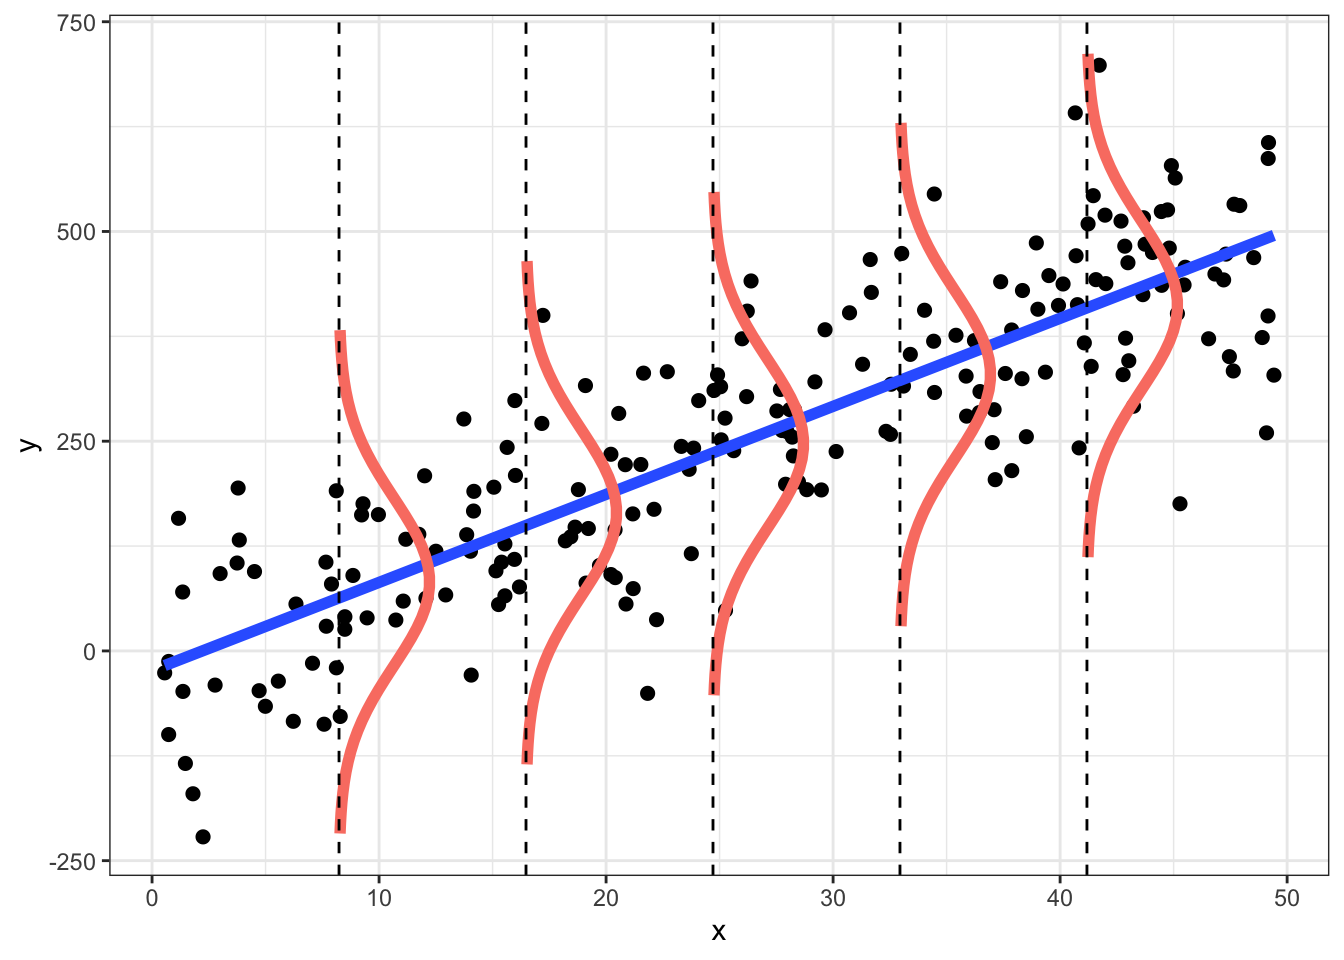
\includegraphics[width=0.8\linewidth]{STAT-5413_files/figure-latex/unnamed-chunk-2-1}

\hypertarget{hierarchical-modeling}{%
\section{Hierarchical modeling}\label{hierarchical-modeling}}

\begin{itemize}
\item
  Follow \citet{berliner1996hierarchical} framework for hierarchical probability models
\item
  Model encodes our understanding of the scientific process of interest
\item
  Model accounts for as much uncertainty as possible
\item
  Model results in a probability distribution

  \begin{itemize}
  \tightlist
  \item
    Note: nature may be deterministic -- often probabilistic models outperform physical models.
  \item
    Example: model individual rain drops vs.~probability/intensity of rain
  \end{itemize}
\item
  Update model with data
\item
  Use the model to generate parameter estimates given data
\end{itemize}

\hypertarget{bayesian-hierarchical-models-bhms}{%
\subsection{Bayesian Hierarchical models (BHMs)}\label{bayesian-hierarchical-models-bhms}}

\begin{itemize}
\item
  Break the model into components:

  \begin{itemize}
  \item
    { Data Model. }
  \item
    { Process Model. }
  \item
    { Parameter Model. }
  \end{itemize}
\item
  Combined, the { data model, } the { process model, } and the { parameter model } define a { posterior distribution. }
\end{itemize}

\begin{align*}
\color{cyan}{[\mathbf{z}, \boldsymbol{\theta}_D, \boldsymbol{\theta}_P | \mathbf{y}]} & \propto
\color{red}{[\mathbf{y} | \boldsymbol{\theta}_D, \mathbf{z}]}  \color{blue}{[\mathbf{z} | \boldsymbol{\theta}_P]} \color{orange}{[\boldsymbol{\theta}_D] [\boldsymbol{\theta}_P]}
\end{align*}

\hypertarget{empirical-hierarchical-models-ehms}{%
\subsection{Empirical Hierarchical models (EHMs)}\label{empirical-hierarchical-models-ehms}}

\begin{itemize}
\item
  Break the model into components:

  \begin{itemize}
  \item
    { Data Model. }
  \item
    { Process Model. }
  \item
    { Parameter estimates } (fixed values) are substituted before fitting the model
  \end{itemize}
\item
  Combined, the { data model and } the { process model } define a { predictive distribution. } Thus, numerical evaluation of the { predictive distribution } is typically required to estimate unceratinty (bootstrap, MLE asymptotics)

  \begin{itemize}
  \tightlist
  \item
    Note: the predictive distribution is not a {posterior distribution} because the normalizing constant is not known
  \end{itemize}
\end{itemize}

\begin{align*}
\color{plum}{[\mathbf{z} | \mathbf{y}]} & \propto
\color{red}{[\mathbf{y} | \boldsymbol{\theta}_D, \mathbf{z}]}  \color{blue}{[\mathbf{z} | \boldsymbol{\theta}_P]}
\end{align*}

\hypertarget{data-model}{%
\subsection{Data Model}\label{data-model}}

\begin{align*}
\color{red}{[\mathbf{y} | \boldsymbol{\theta}_D, \mathbf{z}]}
\end{align*}

\begin{itemize}
\item
  Describes how the data are collected and observed.
\item
  Account for measurement process and uncertainty.
\item
  Model the data in the manner in which they were collected.
\item
  Data \(\mathbf{y}\).

  \begin{itemize}
  \item
    Noisy.
  \item
    Expensive.
  \item
    Not what you want to make inference on.
  \end{itemize}
\item
  Latent variables \(\mathbf{z}\).

  \begin{itemize}
  \item
    Think of \(\mathbf{z}\) as the ideal data.
  \item
    No measurement error - the exact quantity you want to observe but can't.
  \end{itemize}
\item
  Data model parameters \(\boldsymbol{\theta}_D\).
\end{itemize}

\hypertarget{process-model}{%
\subsection{Process Model}\label{process-model}}

\begin{align*}
\color{blue}{[\mathbf{z} | \boldsymbol{\theta}_P]} 
\end{align*}

\begin{itemize}
\item
  \textbf{Where the science happens!}
\item
  Latent process \(\mathbf{z}\) is modeled.
\item
  Can be dynamic in space and/or time
\item
  Process parameters \(\boldsymbol{\theta}_P\).
\item
  Virtually all interesting scientific questions can be made with inference about \(\mathbf{z}\)
\end{itemize}

\hypertarget{parameter-prior-model-bmhs-only}{%
\subsection{Parameter (Prior) Model (BMHs only)}\label{parameter-prior-model-bmhs-only}}

\begin{align*}
\color{orange}{[\boldsymbol{\theta}_D] [\boldsymbol{\theta}_P]}
\end{align*}

\begin{itemize}
\item
  Probability distributions define ``reasonable'' ranges for parameters.
\item
  Parameter models are useful for a variety of problems:

  \begin{itemize}
  \item
    Choosing important variables.
  \item
    Preventing over-fitting (regularization).
  \item
    ``Pooling'' estimates across categories.
  \end{itemize}
\end{itemize}

\hypertarget{posterior-distribution}{%
\subsection{Posterior Distribution}\label{posterior-distribution}}

\begin{align*}
\color{cyan}{[\mathbf{z}, \boldsymbol{\theta}_D, \boldsymbol{\theta}_P | \mathbf{y}]} & \propto
[\mathbf{y} | \boldsymbol{\theta}_D, \mathbf{z}] [\mathbf{z} | \boldsymbol{\theta}_P] [\boldsymbol{\theta}_D] [\boldsymbol{\theta}_P]
\end{align*}

\begin{itemize}
\item
  Probability distribution over all unknowns in the model.
\item
  Inference is made using the posterior distribution.
\item
  Because the posterior distribution is a probability distribution (BHMs), uncertainty is easy to calculate. This is not true for EHMs.
\end{itemize}

\hypertarget{scientifically-motivated-statistical-modeling}{%
\subsection{Scientifically Motivated Statistical Modeling}\label{scientifically-motivated-statistical-modeling}}

\begin{itemize}
\item
  Criticize the model
\item
  Does the model fit the data well?
\item
  Do the predictions make sense?
\item
  Are there subsets of the data that don't fit the model well?
\item
  Make inference using the model.
\item
  If the model fits the data, use the model fit for prediction or inference.
\end{itemize}

\hypertarget{day-2}{%
\chapter{Day 2}\label{day-2}}

\begin{Shaded}
\begin{Highlighting}[]
\KeywordTok{library}\NormalTok{(tidyverse)}
\KeywordTok{library}\NormalTok{(here)}
\KeywordTok{library}\NormalTok{(sp)}
\KeywordTok{library}\NormalTok{(spatstat)}
\end{Highlighting}
\end{Shaded}

\hypertarget{spatial-data}{%
\section{Spatial Data}\label{spatial-data}}

All data occur at some location is space and time. For know we focus on spatial analyses and will later extend this to spatio-temporal analyses. Let \(\mathcal{D}\) represent the spatial domain and let \(\mathbf{s}\) be a spatial location. In general, we will let \(\mathcal{A} \subset \mathcal{D}\) be a subdomain of the spatial region of \(\mathbf{D}\).

\textbf{Insert Diagram from class here}

\hypertarget{types-of-spatial-data}{%
\section{Types of spatial data}\label{types-of-spatial-data}}

There are three primary types of spatial data that we are going to consider

\hypertarget{geostatistical-data}{%
\subsection{Geostatistical data}\label{geostatistical-data}}

\begin{itemize}
\tightlist
\item
  Occur everywhere
\item
  continuous support
\item
  examples: temperature, precipitation
\end{itemize}

\begin{Shaded}
\begin{Highlighting}[]
\KeywordTok{data}\NormalTok{(}\StringTok{"NOAA_df_1990"}\NormalTok{, }\DataTypeTok{package =} \StringTok{"STRbook"}\NormalTok{)}
\KeywordTok{glimpse}\NormalTok{(NOAA_df_}\DecValTok{1990}\NormalTok{)}
\end{Highlighting}
\end{Shaded}

\begin{verbatim}
## Observations: 730,486
## Variables: 10
## $ julian <int> 726834, 726835, 726836, 726837, 726838, 726839, 726840, 7268...
## $ year   <int> 1990, 1990, 1990, 1990, 1990, 1990, 1990, 1990, 1990, 1990, ...
## $ month  <int> 1, 1, 1, 1, 1, 1, 1, 1, 1, 1, 1, 1, 1, 1, 1, 1, 1, 1, 1, 1, ...
## $ day    <int> 1, 2, 3, 4, 5, 6, 7, 8, 9, 10, 11, 12, 13, 14, 15, 16, 17, 1...
## $ id     <dbl> 3804, 3804, 3804, 3804, 3804, 3804, 3804, 3804, 3804, 3804, ...
## $ z      <dbl> 35, 42, 49, 59, 41, 45, 46, 42, 54, 43, 52, 38, 32, 43, 53, ...
## $ proc   <chr> "Tmax", "Tmax", "Tmax", "Tmax", "Tmax", "Tmax", "Tmax", "Tma...
## $ lat    <dbl> 39.35, 39.35, 39.35, 39.35, 39.35, 39.35, 39.35, 39.35, 39.3...
## $ lon    <dbl> -81.43333, -81.43333, -81.43333, -81.43333, -81.43333, -81.4...
## $ date   <date> 1990-01-01, 1990-01-02, 1990-01-03, 1990-01-04, 1990-01-05,...
\end{verbatim}

\begin{Shaded}
\begin{Highlighting}[]
\CommentTok{## Only plot the states with data}
\NormalTok{states <-}\StringTok{ }\KeywordTok{map_data}\NormalTok{(}\StringTok{"state"}\NormalTok{) }
\NormalTok{states <-}\StringTok{ }\NormalTok{states }\OperatorTok
\StringTok{    }\KeywordTok{subset}\NormalTok{(}\OperatorTok{!}\NormalTok{(region }\OperatorTok\StringTok{ }\KeywordTok{c}\NormalTok{(}\StringTok{"washington"}\NormalTok{, }\StringTok{"oregon"}\NormalTok{, }\StringTok{"california"}\NormalTok{, }\StringTok{"nevada"}\NormalTok{, }\StringTok{"idaho"}\NormalTok{, }\StringTok{"utah"}\NormalTok{, }\StringTok{"arizona"}\NormalTok{,}\StringTok{"montana"}\NormalTok{, }\StringTok{"wyoming"}\NormalTok{, }\StringTok{"colorado"}\NormalTok{, }\StringTok{"new mexico"}\NormalTok{))) }

\CommentTok{## generate map}
\NormalTok{NOAA_df_}\DecValTok{1990} \OperatorTok
\StringTok{    }\KeywordTok{subset}\NormalTok{(year }\OperatorTok{==}\StringTok{ }\DecValTok{1990} \OperatorTok{&}\StringTok{ }\NormalTok{day }\OperatorTok{==}\StringTok{ }\DecValTok{1} \OperatorTok{&}\StringTok{ }\NormalTok{proc }\OperatorTok{==}\StringTok{ "Tmax"}\NormalTok{) }\OperatorTok\StringTok{   }
\StringTok{    }\KeywordTok{ggplot}\NormalTok{(}\KeywordTok{aes}\NormalTok{(}\DataTypeTok{x =}\NormalTok{ lon, }\DataTypeTok{y =}\NormalTok{ lat, }\DataTypeTok{color =}\NormalTok{ z)) }\OperatorTok{+}
\StringTok{    }\KeywordTok{geom_point}\NormalTok{() }\OperatorTok{+}\StringTok{ }
\StringTok{    }\KeywordTok{facet_wrap}\NormalTok{(}\OperatorTok{~}\StringTok{ }\NormalTok{month, }\DataTypeTok{scales =} \StringTok{"free"}\NormalTok{, }\DataTypeTok{nrow =} \DecValTok{4}\NormalTok{) }\OperatorTok{+}
\StringTok{    }\KeywordTok{geom_polygon}\NormalTok{(}\DataTypeTok{data =}\NormalTok{ states, }\KeywordTok{aes}\NormalTok{(}\DataTypeTok{x =}\NormalTok{ long, }\DataTypeTok{y =}\NormalTok{ lat, }\DataTypeTok{group =}\NormalTok{ group), }
                 \DataTypeTok{inherit.aes =} \OtherTok{FALSE}\NormalTok{, }\DataTypeTok{fill =} \OtherTok{NA}\NormalTok{, }\DataTypeTok{color =} \StringTok{"black"}\NormalTok{) }\OperatorTok{+}
\StringTok{    }\KeywordTok{scale_color_viridis_c}\NormalTok{(}\DataTypeTok{option =} \StringTok{"inferno"}\NormalTok{) }\OperatorTok{+}
\StringTok{    }\KeywordTok{ggtitle}\NormalTok{(}\StringTok{"Tmax for the first day of each month in 1990"}\NormalTok{)}
\end{Highlighting}
\end{Shaded}

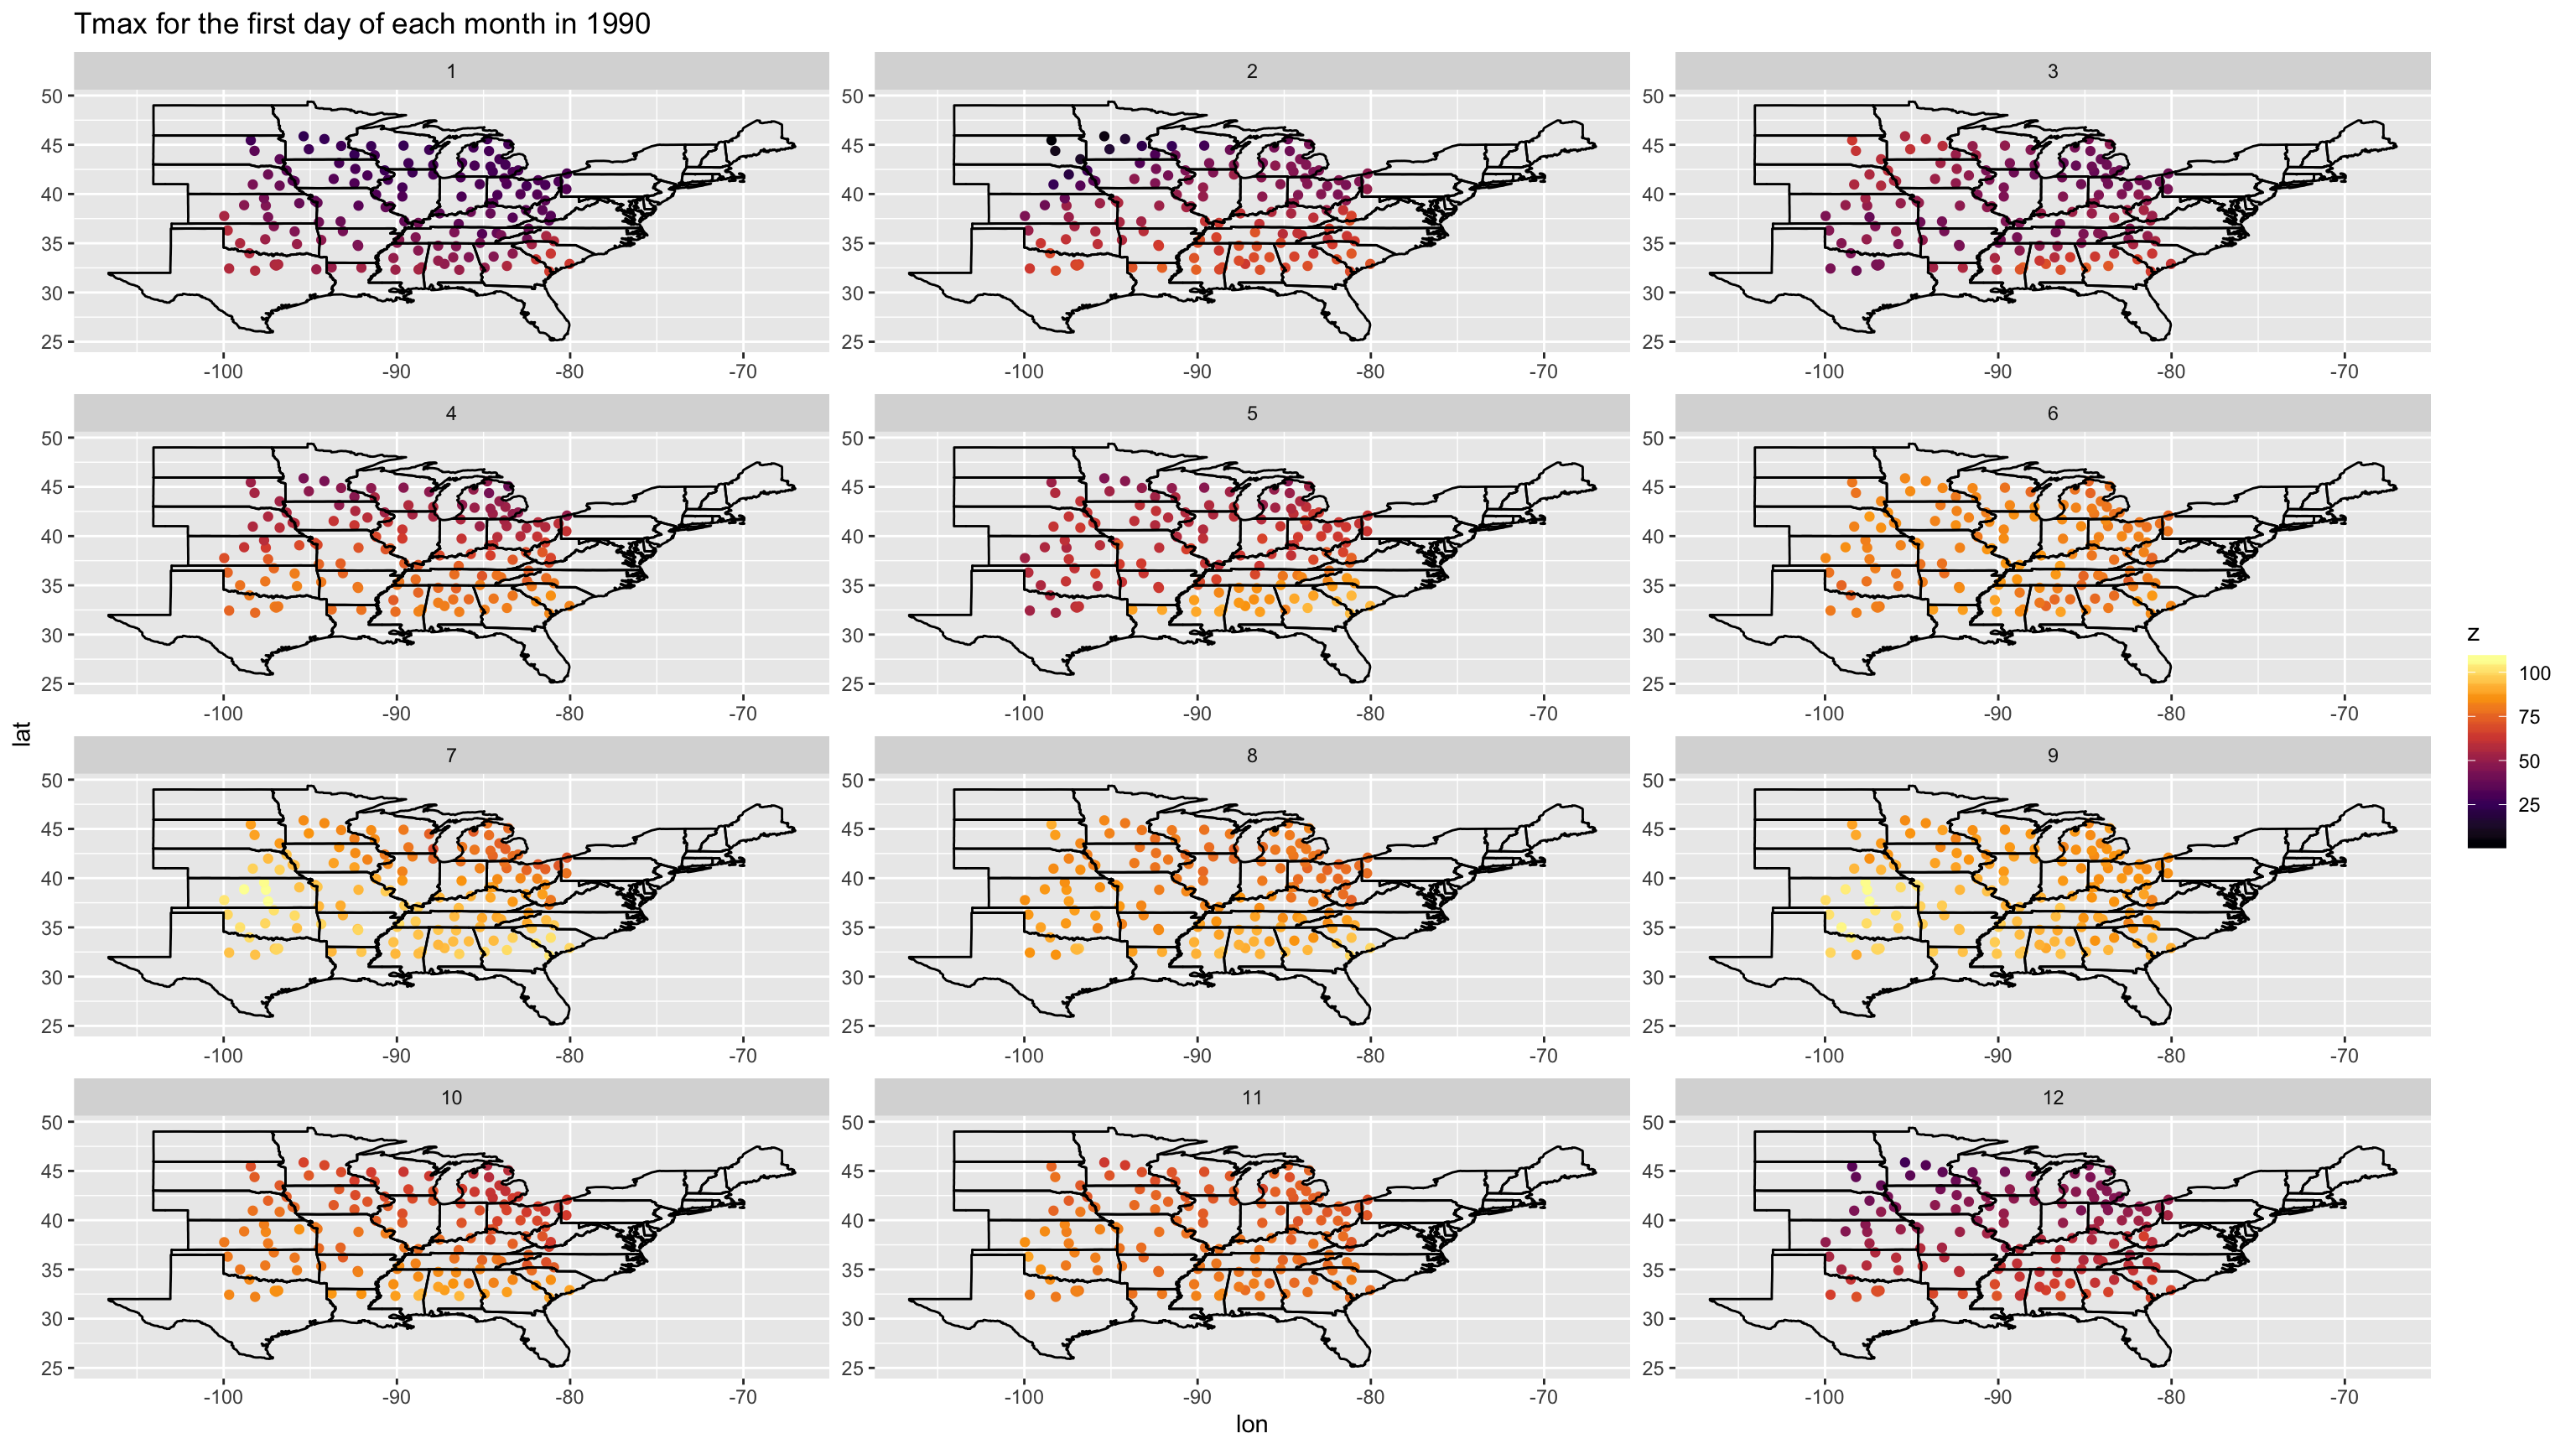
\includegraphics{STAT-5413_files/figure-latex/unnamed-chunk-5-1.pdf}

\hypertarget{areal-data}{%
\subsection{Areal data}\label{areal-data}}

\begin{itemize}
\tightlist
\item
  Occur only over discrete areas
\item
  can be thought of as an integral of a continuous process over a subdomain \(\mathcal{A} \in \mathcal{D}\)
\item
  examples: cases of a disease by counties, votes in an election by congressional district
\end{itemize}

\begin{Shaded}
\begin{Highlighting}[]
\KeywordTok{data}\NormalTok{(}\StringTok{"BEA"}\NormalTok{, }\DataTypeTok{package =} \StringTok{"STRbook"}\NormalTok{)}
\KeywordTok{glimpse}\NormalTok{(BEA)}
\end{Highlighting}
\end{Shaded}

\begin{verbatim}
## Observations: 116
## Variables: 5
## $ Description <chr> "Per capita personal income (dollars)", "Per capita per...
## $ NAME10      <fct> "Adair, MO", "Andrew, MO", "Atchison, MO", "Audrain, MO...
## $ X1970       <int> 2723, 3577, 3770, 3678, 3021, 2832, 3263, 2508, 2147, 3...
## $ X1980       <int> 7399, 7937, 5743, 8356, 7210, 7445, 8596, 6125, 5431, 9...
## $ X1990       <int> 12755, 15059, 14748, 15198, 12873, 13530, 13195, 11854,...
\end{verbatim}

\begin{Shaded}
\begin{Highlighting}[]
\KeywordTok{data}\NormalTok{(}\StringTok{"MOcounties"}\NormalTok{, }\DataTypeTok{package =} \StringTok{"STRbook"}\NormalTok{)}
\KeywordTok{glimpse}\NormalTok{(MOcounties)}
\end{Highlighting}
\end{Shaded}

\begin{verbatim}
## Observations: 214,279
## Variables: 53
## $ long       <dbl> 627911.9, 627921.4, 627923.0, 627947.8, 627956.5, 627994...
## $ lat        <dbl> 4473554, 4473559, 4473560, 4473577, 4473583, 4473612, 44...
## $ order      <int> 1, 2, 3, 4, 5, 6, 7, 8, 9, 10, 11, 12, 13, 14, 15, 16, 1...
## $ hole       <lgl> FALSE, FALSE, FALSE, FALSE, FALSE, FALSE, FALSE, FALSE, ...
## $ piece      <fct> 1, 1, 1, 1, 1, 1, 1, 1, 1, 1, 1, 1, 1, 1, 1, 1, 1, 1, 1,...
## $ id         <chr> "0", "0", "0", "0", "0", "0", "0", "0", "0", "0", "0", "...
## $ group      <fct> 0.1, 0.1, 0.1, 0.1, 0.1, 0.1, 0.1, 0.1, 0.1, 0.1, 0.1, 0...
## $ STATEFP10  <fct> 29, 29, 29, 29, 29, 29, 29, 29, 29, 29, 29, 29, 29, 29, ...
## $ COUNTYFP10 <fct> 045, 045, 045, 045, 045, 045, 045, 045, 045, 045, 045, 0...
## $ COUNTYNS10 <fct> 00758477, 00758477, 00758477, 00758477, 00758477, 007584...
## $ GEOID10    <fct> 29045, 29045, 29045, 29045, 29045, 29045, 29045, 29045, ...
## $ NAME10     <fct> "Clark, MO", "Clark, MO", "Clark, MO", "Clark, MO", "Cla...
## $ NAMELSAD10 <fct> Clark County, Clark County, Clark County, Clark County, ...
## $ LSAD10     <fct> 06, 06, 06, 06, 06, 06, 06, 06, 06, 06, 06, 06, 06, 06, ...
## $ CLASSFP10  <fct> H1, H1, H1, H1, H1, H1, H1, H1, H1, H1, H1, H1, H1, H1, ...
## $ MTFCC10    <fct> G4020, G4020, G4020, G4020, G4020, G4020, G4020, G4020, ...
## $ CSAFP10    <fct> NA, NA, NA, NA, NA, NA, NA, NA, NA, NA, NA, NA, NA, NA, ...
## $ CBSAFP10   <fct> 22800, 22800, 22800, 22800, 22800, 22800, 22800, 22800, ...
## $ METDIVFP10 <fct> NA, NA, NA, NA, NA, NA, NA, NA, NA, NA, NA, NA, NA, NA, ...
## $ FUNCSTAT10 <fct> A, A, A, A, A, A, A, A, A, A, A, A, A, A, A, A, A, A, A,...
## $ ALAND10    <dbl> 1307146971, 1307146971, 1307146971, 1307146971, 13071469...
## $ AWATER10   <dbl> 18473547, 18473547, 18473547, 18473547, 18473547, 184735...
## $ INTPTLAT10 <fct> +40.4072748, +40.4072748, +40.4072748, +40.4072748, +40....
## $ INTPTLON10 <fct> -091.7294720, -091.7294720, -091.7294720, -091.7294720, ...
## $ AREA       <dbl> 1324937990, 1324937990, 1324937990, 1324937990, 13249379...
## $ PERIMETER  <dbl> 161503.6, 161503.6, 161503.6, 161503.6, 161503.6, 161503...
## $ COUNTY10_  <int> 2, 2, 2, 2, 2, 2, 2, 2, 2, 2, 2, 2, 2, 2, 2, 2, 2, 2, 2,...
## $ COUNTY10_I <int> 115, 115, 115, 115, 115, 115, 115, 115, 115, 115, 115, 1...
## $ POP90      <int> 7547, 7547, 7547, 7547, 7547, 7547, 7547, 7547, 7547, 75...
## $ WHITE90    <int> 7528, 7528, 7528, 7528, 7528, 7528, 7528, 7528, 7528, 75...
## $ BLACK90    <int> 3, 3, 3, 3, 3, 3, 3, 3, 3, 3, 3, 3, 3, 3, 3, 3, 3, 3, 3,...
## $ ASIANPI90  <int> 4, 4, 4, 4, 4, 4, 4, 4, 4, 4, 4, 4, 4, 4, 4, 4, 4, 4, 4,...
## $ AMIND90    <int> 7, 7, 7, 7, 7, 7, 7, 7, 7, 7, 7, 7, 7, 7, 7, 7, 7, 7, 7,...
## $ OTHER90    <int> 5, 5, 5, 5, 5, 5, 5, 5, 5, 5, 5, 5, 5, 5, 5, 5, 5, 5, 5,...
## $ HISP90     <int> 26, 26, 26, 26, 26, 26, 26, 26, 26, 26, 26, 26, 26, 26, ...
## $ POP00      <int> 7416, 7416, 7416, 7416, 7416, 7416, 7416, 7416, 7416, 74...
## $ WHITE00    <int> 7329, 7329, 7329, 7329, 7329, 7329, 7329, 7329, 7329, 73...
## $ BLACK00    <int> 5, 5, 5, 5, 5, 5, 5, 5, 5, 5, 5, 5, 5, 5, 5, 5, 5, 5, 5,...
## $ ASIAN00    <int> 5, 5, 5, 5, 5, 5, 5, 5, 5, 5, 5, 5, 5, 5, 5, 5, 5, 5, 5,...
## $ AMIND00    <int> 15, 15, 15, 15, 15, 15, 15, 15, 15, 15, 15, 15, 15, 15, ...
## $ HAWNPI00   <int> 1, 1, 1, 1, 1, 1, 1, 1, 1, 1, 1, 1, 1, 1, 1, 1, 1, 1, 1,...
## $ OTHER00    <int> 16, 16, 16, 16, 16, 16, 16, 16, 16, 16, 16, 16, 16, 16, ...
## $ MULTRA00   <int> 45, 45, 45, 45, 45, 45, 45, 45, 45, 45, 45, 45, 45, 45, ...
## $ HISP00     <int> 52, 52, 52, 52, 52, 52, 52, 52, 52, 52, 52, 52, 52, 52, ...
## $ POP10      <int> 7139, 7139, 7139, 7139, 7139, 7139, 7139, 7139, 7139, 71...
## $ WHITE10    <int> 7011, 7011, 7011, 7011, 7011, 7011, 7011, 7011, 7011, 70...
## $ BLACK10    <int> 19, 19, 19, 19, 19, 19, 19, 19, 19, 19, 19, 19, 19, 19, ...
## $ ASIAN10    <int> 23, 23, 23, 23, 23, 23, 23, 23, 23, 23, 23, 23, 23, 23, ...
## $ AMIND10    <int> 9, 9, 9, 9, 9, 9, 9, 9, 9, 9, 9, 9, 9, 9, 9, 9, 9, 9, 9,...
## $ HAWNPI10   <int> 0, 0, 0, 0, 0, 0, 0, 0, 0, 0, 0, 0, 0, 0, 0, 0, 0, 0, 0,...
## $ OTHER10    <int> 5, 5, 5, 5, 5, 5, 5, 5, 5, 5, 5, 5, 5, 5, 5, 5, 5, 5, 5,...
## $ MULTRA10   <int> 72, 72, 72, 72, 72, 72, 72, 72, 72, 72, 72, 72, 72, 72, ...
## $ HISP10     <int> 42, 42, 42, 42, 42, 42, 42, 42, 42, 42, 42, 42, 42, 42, ...
\end{verbatim}

\begin{Shaded}
\begin{Highlighting}[]
\NormalTok{MOcounties <-}\StringTok{ }\KeywordTok{left_join}\NormalTok{(MOcounties, BEA, }\DataTypeTok{by =} \StringTok{"NAME10"}\NormalTok{)}
\end{Highlighting}
\end{Shaded}

\begin{Shaded}
\begin{Highlighting}[]
\KeywordTok{ggplot}\NormalTok{(MOcounties) }\OperatorTok{+}
\StringTok{    }\KeywordTok{geom_polygon}\NormalTok{(}\KeywordTok{aes}\NormalTok{(}\DataTypeTok{x =}\NormalTok{ long,}
                     \DataTypeTok{y =}\NormalTok{ lat, }\CommentTok{# county boundary}
                     \DataTypeTok{group =}\NormalTok{ NAME10, }\CommentTok{# county group}
                     \DataTypeTok{fill =} \KeywordTok{log}\NormalTok{(X1970))) }\OperatorTok{+}\StringTok{ }\CommentTok{# log of income}
\StringTok{    }\KeywordTok{geom_path}\NormalTok{(}\KeywordTok{aes}\NormalTok{(}\DataTypeTok{x =}\NormalTok{ long, }\DataTypeTok{y =}\NormalTok{ lat, }\DataTypeTok{group =}\NormalTok{ NAME10)) }\OperatorTok{+}
\StringTok{    }\KeywordTok{scale_fill_viridis_c}\NormalTok{(}\DataTypeTok{limits =} \KeywordTok{c}\NormalTok{(}\FloatTok{7.5}\NormalTok{, }\FloatTok{10.2}\NormalTok{), }\DataTypeTok{option =} \StringTok{"plasma"}\NormalTok{, }\DataTypeTok{name =} \StringTok{"log($)"}\NormalTok{) }\OperatorTok{+}
\StringTok{    }\KeywordTok{coord_fixed}\NormalTok{() }\OperatorTok{+}\StringTok{ }
\StringTok{    }\KeywordTok{ggtitle}\NormalTok{(}\StringTok{"1970"}\NormalTok{) }\OperatorTok{+}
\StringTok{    }\KeywordTok{xlab}\NormalTok{(}\StringTok{"x (m)"}\NormalTok{) }\OperatorTok{+}
\StringTok{    }\KeywordTok{ylab}\NormalTok{(}\StringTok{"y (m)"}\NormalTok{) }\OperatorTok{+}
\StringTok{    }\KeywordTok{theme_bw}\NormalTok{()}
\end{Highlighting}
\end{Shaded}

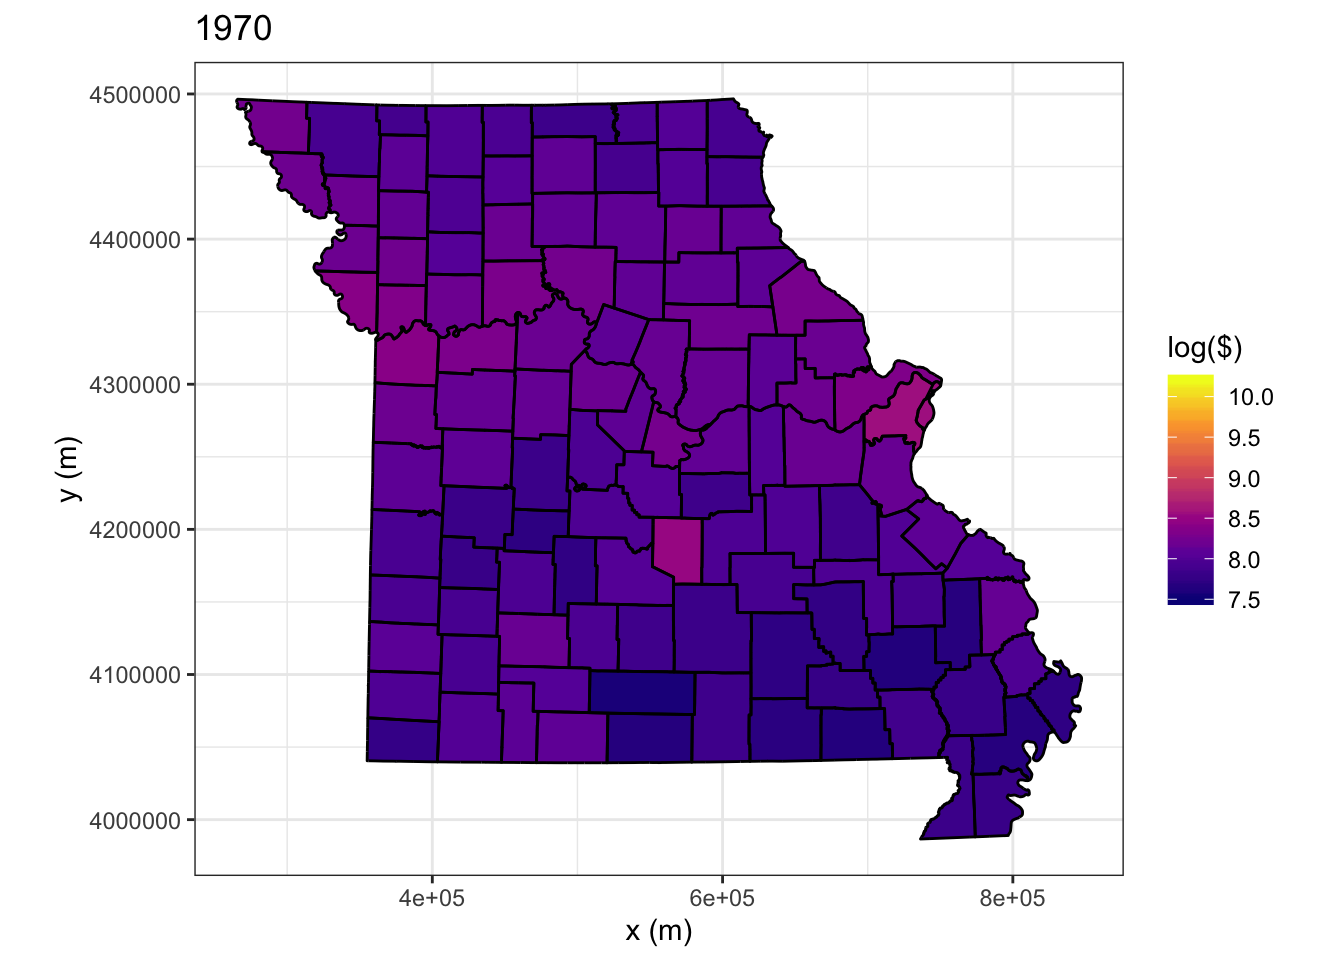
\includegraphics{STAT-5413_files/figure-latex/unnamed-chunk-7-1.pdf}

\hypertarget{point-process-data}{%
\subsection{Point process data}\label{point-process-data}}

\begin{itemize}
\tightlist
\item
  The count and location of the data are random
\item
  examples: tornados, lightning strikes
\end{itemize}

\begin{Shaded}
\begin{Highlighting}[]
\CommentTok{# uncomment out this line to download the data}
\CommentTok{# load(url("http://github.com/mgimond/Spatial/raw/master/Data/ppa.RData"))}
\CommentTok{# save(starbucks, ma, pop, file = here::here("data", "ppa-starbucks.RData"))}
\KeywordTok{load}\NormalTok{(here}\OperatorTok{::}\KeywordTok{here}\NormalTok{(}\StringTok{"data"}\NormalTok{, }\StringTok{"ppa-starbucks.RData"}\NormalTok{))}
\KeywordTok{glimpse}\NormalTok{(starbucks)}
\end{Highlighting}
\end{Shaded}

\begin{verbatim}
## List of 5
##  $ window    :List of 4
##   ..$ type  : chr "rectangle"
##   ..$ xrange: num [1:2] 648032 917741
##   ..$ yrange: num [1:2] 4609785 4748107
##   ..$ units :List of 3
##   .. ..$ singular  : chr "unit"
##   .. ..$ plural    : chr "units"
##   .. ..$ multiplier: num 1
##   .. ..- attr(*, "class")= chr "unitname"
##   ..- attr(*, "class")= chr "owin"
##  $ n         : int 171
##  $ x         : num [1:171] 917741 911147 902987 876188 875868 ...
##  $ y         : num [1:171] 4637151 4628510 4628982 4616741 4616719 ...
##  $ markformat: chr "none"
##  - attr(*, "class")= chr "ppp"
\end{verbatim}

\begin{Shaded}
\begin{Highlighting}[]
\CommentTok{## uses spatstat library}
\CommentTok{## add the massachusetts polygon}
\KeywordTok{Window}\NormalTok{(starbucks) <-}\StringTok{ }\NormalTok{ma}
\KeywordTok{marks}\NormalTok{(starbucks) <-}\StringTok{ }\OtherTok{NULL}
\CommentTok{## plot using the plot function from spatstat}
\KeywordTok{plot}\NormalTok{(starbucks)}
\end{Highlighting}
\end{Shaded}

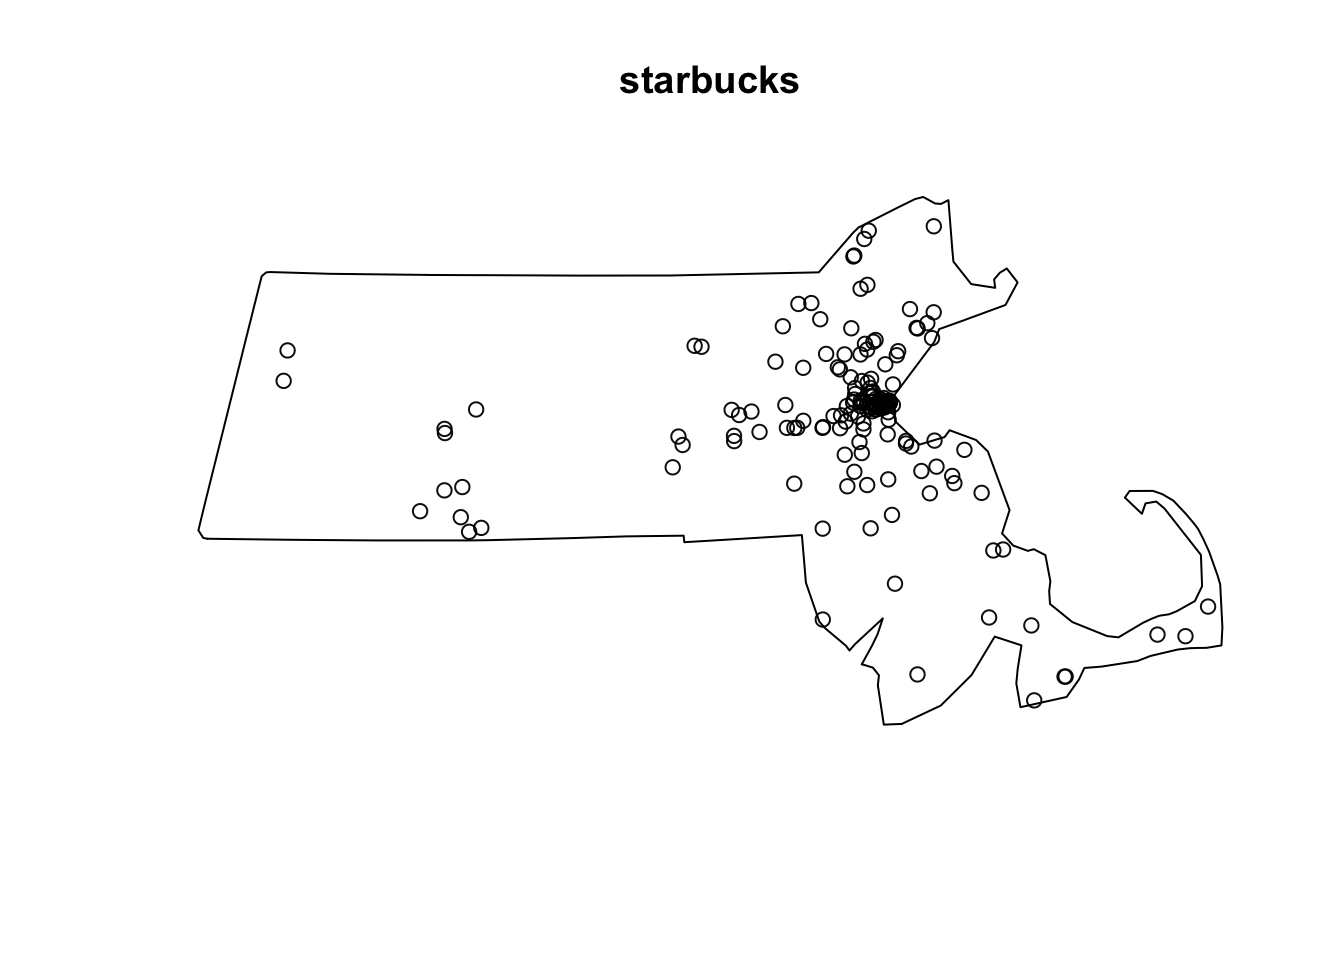
\includegraphics{STAT-5413_files/figure-latex/unnamed-chunk-9-1.pdf}

\hypertarget{day-3}{%
\chapter{Day 3}\label{day-3}}

\begin{Shaded}
\begin{Highlighting}[]
\KeywordTok{library}\NormalTok{(tidyverse)}
\KeywordTok{library}\NormalTok{(here)}
\KeywordTok{library}\NormalTok{(sp)}
\end{Highlighting}
\end{Shaded}

\hypertarget{anouncements}{%
\section{Anouncements}\label{anouncements}}

\begin{itemize}
\item
  Show gitHub page for site \url{https://github.com/jtipton25/STAT-5413}

  \begin{itemize}
  \tightlist
  \item
    Show how to download files and data
  \end{itemize}
\end{itemize}

\hypertarget{files-for-spatial-data}{%
\section{Files for spatial data}\label{files-for-spatial-data}}

\begin{itemize}
\item
  Many different file types for spatial data
\item
  Typically data are in ``flat files'' like comma-seperated value (CSV) files
\end{itemize}

\begin{Shaded}
\begin{Highlighting}[]
\KeywordTok{read.csv}\NormalTok{(}\KeywordTok{here}\NormalTok{(}\StringTok{"path"}\NormalTok{, }\StringTok{"to"}\NormalTok{, }\StringTok{"file.csv"}\NormalTok{))}
\end{Highlighting}
\end{Shaded}

\begin{itemize}
\tightlist
\item
  ``shapefiles'' which can be read using \emph{rgdal} or \emph{maptools} packages
\end{itemize}

\begin{Shaded}
\begin{Highlighting}[]
\KeywordTok{library}\NormalTok{(rgdal)}
\KeywordTok{library}\NormalTok{(maptools)}
\end{Highlighting}
\end{Shaded}

\begin{itemize}
\tightlist
\item
  ``NetCDF'' files cane be read using \emph{ncdf4} or \emph{RNetCDF}
\end{itemize}

\begin{Shaded}
\begin{Highlighting}[]
\KeywordTok{library}\NormalTok{(ncdf4)}
\KeywordTok{library}\NormalTok{(RNetCDF)}
\end{Highlighting}
\end{Shaded}

\hypertarget{textbook-package}{%
\section{Textbook package}\label{textbook-package}}

To install the data from the textbook, go to \url{https://spacetimewithr.org/} and follow the link to the code.

\begin{Shaded}
\begin{Highlighting}[]
\CommentTok{# install.packages("devtools")}
\KeywordTok{library}\NormalTok{(devtools)}
\KeywordTok{install_github}\NormalTok{(}\StringTok{"andrewzm/STRbook"}\NormalTok{)}
\end{Highlighting}
\end{Shaded}

Note that this package is relatively large because it contains a decent amount of spatial data.

\begin{Shaded}
\begin{Highlighting}[]
\KeywordTok{library}\NormalTok{(STRbook)}
\end{Highlighting}
\end{Shaded}

\begin{verbatim}
## 
## Attaching package: 'STRbook'
\end{verbatim}

\begin{verbatim}
## The following object is masked _by_ '.GlobalEnv':
## 
##     MOcounties
\end{verbatim}

\hypertarget{spatial-visualization}{%
\section{Spatial Visualization}\label{spatial-visualization}}

\hypertarget{spatial-visualization-using-fields}{%
\subsection{\texorpdfstring{Spatial visualization using \emph{fields}}{Spatial visualization using fields}}\label{spatial-visualization-using-fields}}

\begin{itemize}
\tightlist
\item
  Simulate a process with some random locations
\end{itemize}

\begin{Shaded}
\begin{Highlighting}[]
\KeywordTok{library}\NormalTok{(fields)}
\end{Highlighting}
\end{Shaded}

\begin{verbatim}
## Loading required package: spam
\end{verbatim}

\begin{verbatim}
## Loading required package: dotCall64
\end{verbatim}

\begin{verbatim}
## Loading required package: grid
\end{verbatim}

\begin{verbatim}
## Spam version 2.5-1 (2019-12-12) is loaded.
## Type 'help( Spam)' or 'demo( spam)' for a short introduction 
## and overview of this package.
## Help for individual functions is also obtained by adding the
## suffix '.spam' to the function name, e.g. 'help( chol.spam)'.
\end{verbatim}

\begin{verbatim}
## 
## Attaching package: 'spam'
\end{verbatim}

\begin{verbatim}
## The following objects are masked from 'package:base':
## 
##     backsolve, forwardsolve
\end{verbatim}

\begin{verbatim}
## Loading required package: maps
\end{verbatim}

\begin{verbatim}
## 
## Attaching package: 'maps'
\end{verbatim}

\begin{verbatim}
## The following object is masked from 'package:purrr':
## 
##     map
\end{verbatim}

\begin{verbatim}
## See https://github.com/NCAR/Fields for
##  an extensive vignette, other supplements and source code
\end{verbatim}

\begin{Shaded}
\begin{Highlighting}[]
\CommentTok{## longitude and latitude of approximately the center of Arkansas}
\NormalTok{lon_lat_center <-}\StringTok{ }\KeywordTok{c}\NormalTok{(}\OperatorTok{-}\FloatTok{92.33}\NormalTok{, }\FloatTok{35.00}\NormalTok{) }

\NormalTok{n   <-}\StringTok{ }\DecValTok{1000}
\CommentTok{## simulate some random locations}
\NormalTok{lon  <-}\StringTok{ }\KeywordTok{runif}\NormalTok{(n, lon_lat_center[}\DecValTok{1}\NormalTok{] }\OperatorTok{-}\StringTok{ }\DecValTok{2}\NormalTok{, lon_lat_center[}\DecValTok{1}\NormalTok{] }\OperatorTok{+}\StringTok{ }\DecValTok{2}\NormalTok{)}
\NormalTok{lat  <-}\StringTok{ }\KeywordTok{runif}\NormalTok{(n, lon_lat_center[}\DecValTok{2}\NormalTok{] }\OperatorTok{-}\StringTok{ }\DecValTok{2}\NormalTok{, lon_lat_center[}\DecValTok{2}\NormalTok{] }\OperatorTok{+}\StringTok{ }\DecValTok{2}\NormalTok{)}
\NormalTok{y   <-}\StringTok{ }\KeywordTok{rnorm}\NormalTok{(n, lat }\OperatorTok{+}\StringTok{ }\NormalTok{lon, }\FloatTok{.1}\NormalTok{)}

\KeywordTok{plot}\NormalTok{(lon, lat)}
\end{Highlighting}
\end{Shaded}

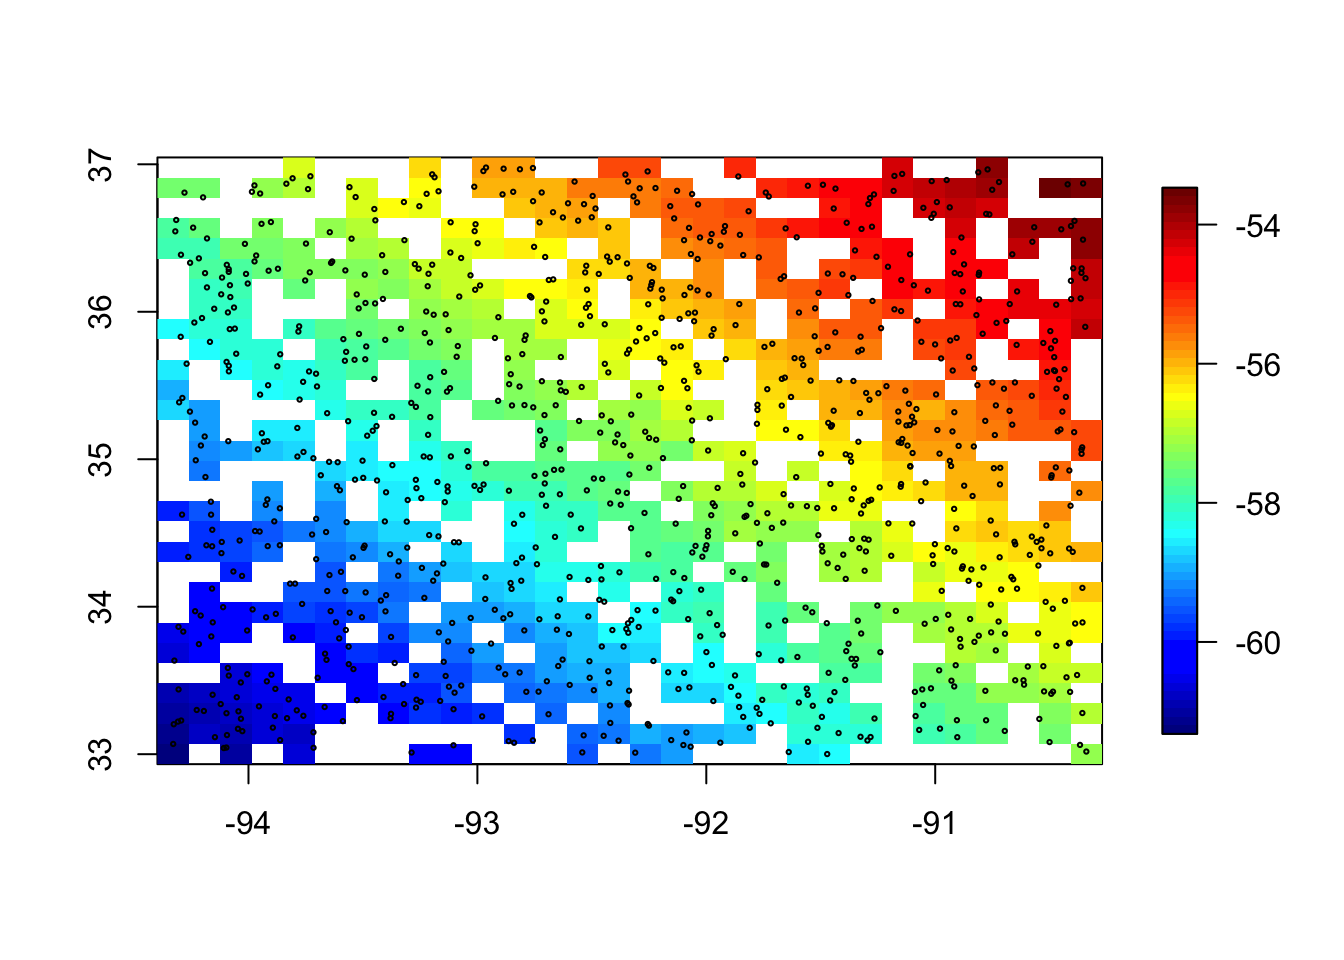
\includegraphics{STAT-5413_files/figure-latex/unnamed-chunk-16-1.pdf}

\begin{Shaded}
\begin{Highlighting}[]
\KeywordTok{quilt.plot}\NormalTok{(lon, lat, y, }\DataTypeTok{nx =} \DecValTok{30}\NormalTok{, }\DataTypeTok{ny =} \DecValTok{30}\NormalTok{)}
\KeywordTok{points}\NormalTok{(lon, lat, }\DataTypeTok{cex =} \FloatTok{.3}\NormalTok{)}
\end{Highlighting}
\end{Shaded}

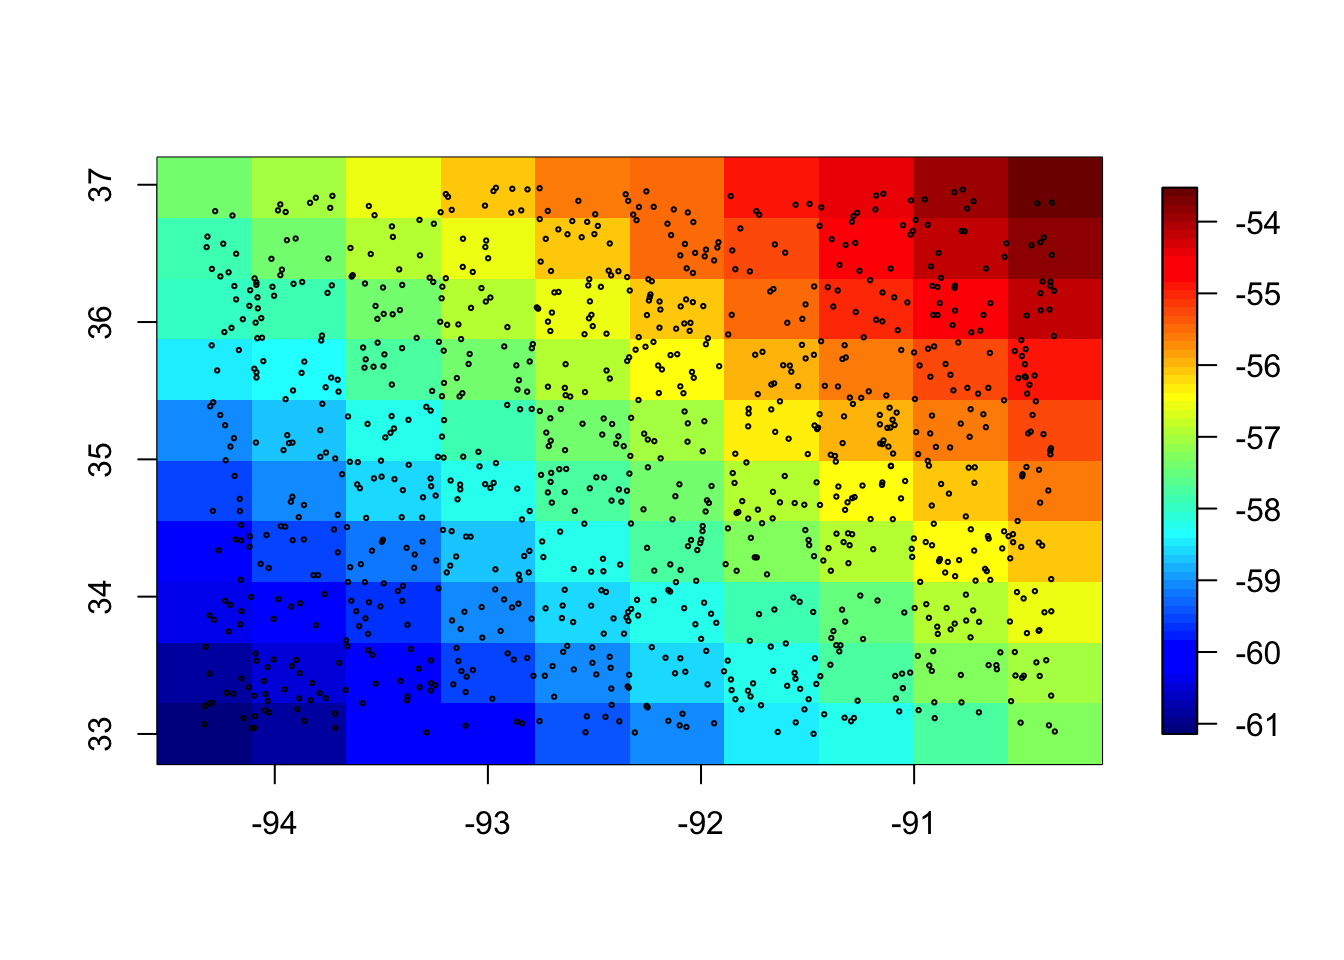
\includegraphics{STAT-5413_files/figure-latex/unnamed-chunk-17-1.pdf}

\begin{Shaded}
\begin{Highlighting}[]
\KeywordTok{quilt.plot}\NormalTok{(lon, lat, y, }\DataTypeTok{nx =} \DecValTok{10}\NormalTok{, }\DataTypeTok{ny =} \DecValTok{10}\NormalTok{)}
\KeywordTok{points}\NormalTok{(lon, lat, }\DataTypeTok{cex =} \FloatTok{.3}\NormalTok{)}
\end{Highlighting}
\end{Shaded}

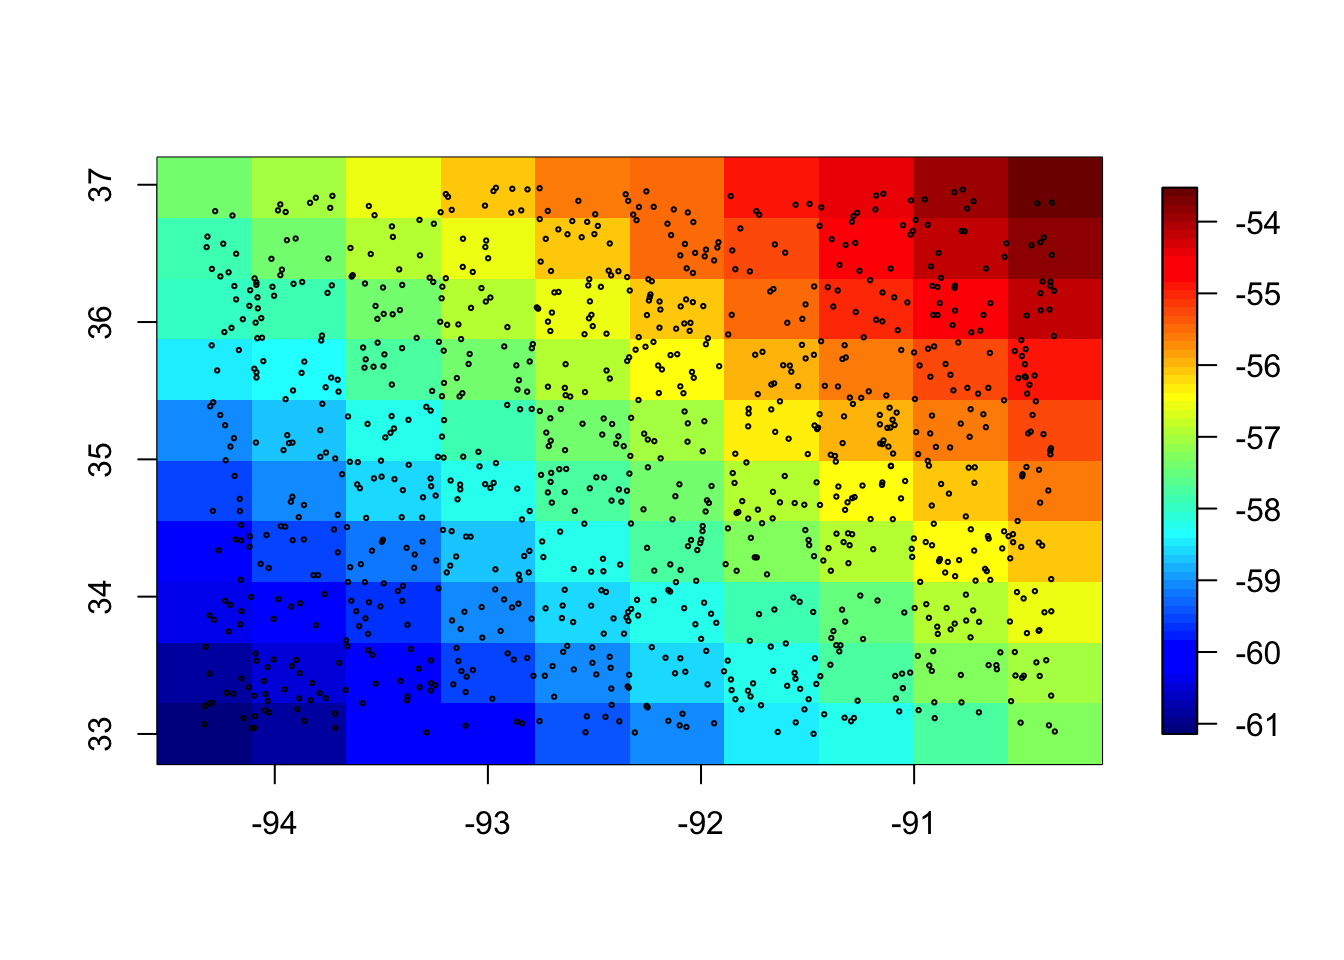
\includegraphics{STAT-5413_files/figure-latex/unnamed-chunk-18-1.pdf}

\begin{itemize}
\tightlist
\item
  Simulate a process on a regular grid
\end{itemize}

\begin{Shaded}
\begin{Highlighting}[]
\NormalTok{n <-}\StringTok{ }\DecValTok{50}\OperatorTok{^}\DecValTok{2}
\CommentTok{## simulate locations on a grid}
\NormalTok{lon  <-}\StringTok{ }\KeywordTok{seq}\NormalTok{(lon_lat_center[}\DecValTok{1}\NormalTok{] }\OperatorTok{-}\StringTok{ }\DecValTok{2}\NormalTok{, lon_lat_center[}\DecValTok{1}\NormalTok{] }\OperatorTok{+}\StringTok{ }\DecValTok{2}\NormalTok{, }\DataTypeTok{length =} \KeywordTok{sqrt}\NormalTok{(n))}
\NormalTok{lat  <-}\StringTok{ }\KeywordTok{seq}\NormalTok{(lon_lat_center[}\DecValTok{2}\NormalTok{] }\OperatorTok{-}\StringTok{ }\DecValTok{2}\NormalTok{, lon_lat_center[}\DecValTok{2}\NormalTok{] }\OperatorTok{+}\StringTok{ }\DecValTok{2}\NormalTok{, }\DataTypeTok{length =} \KeywordTok{sqrt}\NormalTok{(n))}
\NormalTok{s <-}\StringTok{ }\KeywordTok{expand.grid}\NormalTok{(lon, lat)}

\KeywordTok{head}\NormalTok{(lon)}
\end{Highlighting}
\end{Shaded}

\begin{verbatim}
## [1] -94.33000 -94.24837 -94.16673 -94.08510 -94.00347 -93.92184
\end{verbatim}

\begin{Shaded}
\begin{Highlighting}[]
\KeywordTok{head}\NormalTok{(lat)}
\end{Highlighting}
\end{Shaded}

\begin{verbatim}
## [1] 33.00000 33.08163 33.16327 33.24490 33.32653 33.40816
\end{verbatim}

\begin{Shaded}
\begin{Highlighting}[]
\KeywordTok{head}\NormalTok{(s)}
\end{Highlighting}
\end{Shaded}

\begin{verbatim}
##        Var1 Var2
## 1 -94.33000   33
## 2 -94.24837   33
## 3 -94.16673   33
## 4 -94.08510   33
## 5 -94.00347   33
## 6 -93.92184   33
\end{verbatim}

\begin{Shaded}
\begin{Highlighting}[]
\KeywordTok{plot}\NormalTok{(s, }\DataTypeTok{cex =} \FloatTok{0.3}\NormalTok{)}
\end{Highlighting}
\end{Shaded}

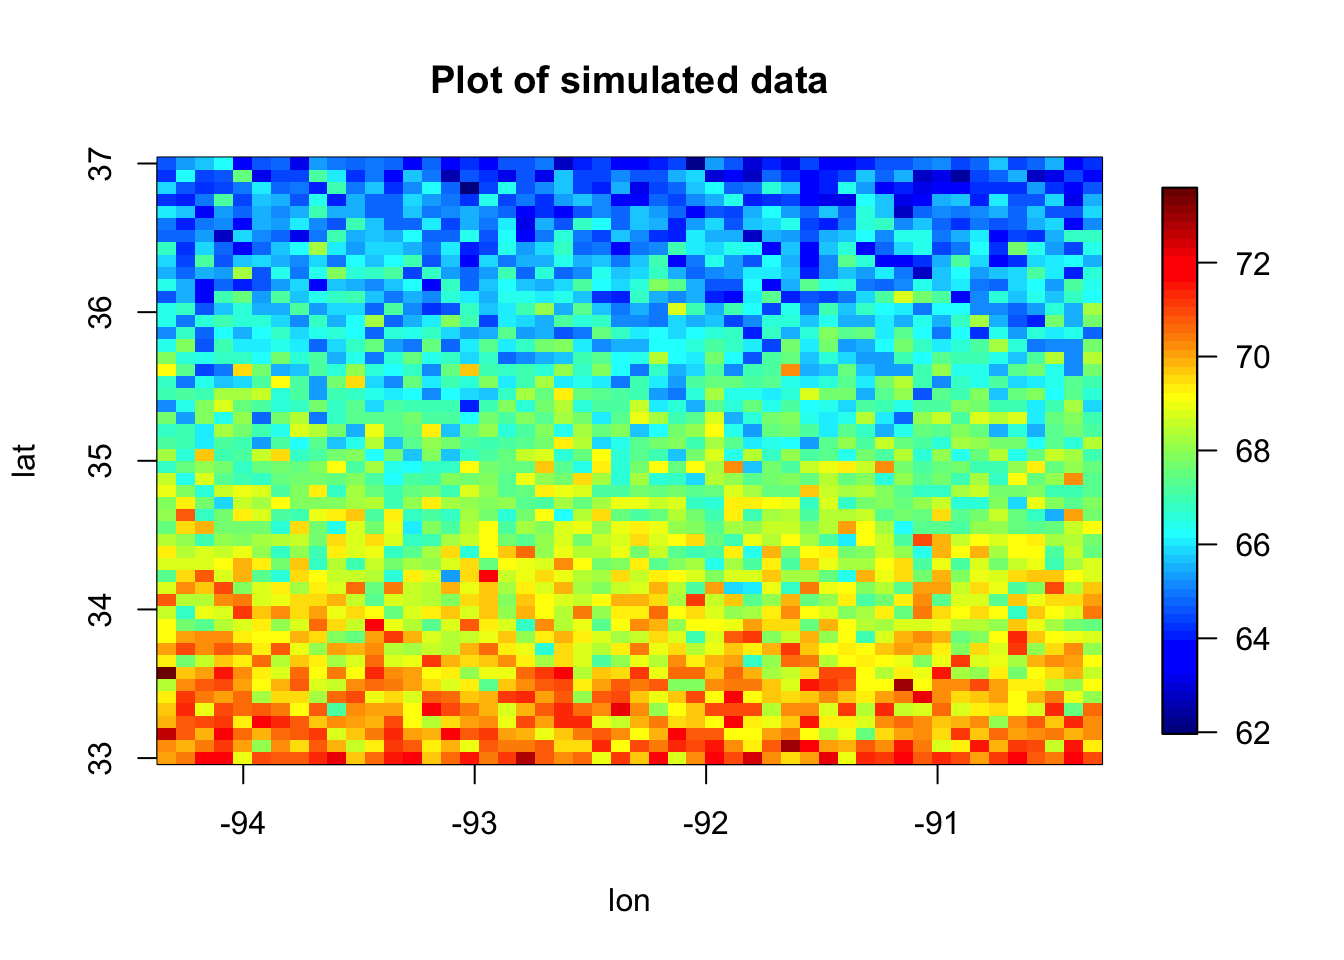
\includegraphics{STAT-5413_files/figure-latex/unnamed-chunk-19-1.pdf}

\begin{Shaded}
\begin{Highlighting}[]
\CommentTok{## simulate some fake data with a north/south trend}
\NormalTok{y <-}\StringTok{ }\DecValTok{120} \OperatorTok{-}\StringTok{ }\FloatTok{1.5} \OperatorTok{*}\StringTok{ }\NormalTok{s[, }\DecValTok{2}\NormalTok{] }\OperatorTok{+}\StringTok{ }\KeywordTok{matrix}\NormalTok{(}\KeywordTok{rnorm}\NormalTok{(n), }\KeywordTok{sqrt}\NormalTok{(n), }\KeywordTok{sqrt}\NormalTok{(n))}
\KeywordTok{image.plot}\NormalTok{(lon, lat, y, }\DataTypeTok{main =} \StringTok{"Plot of simulated data"}\NormalTok{)}
\end{Highlighting}
\end{Shaded}

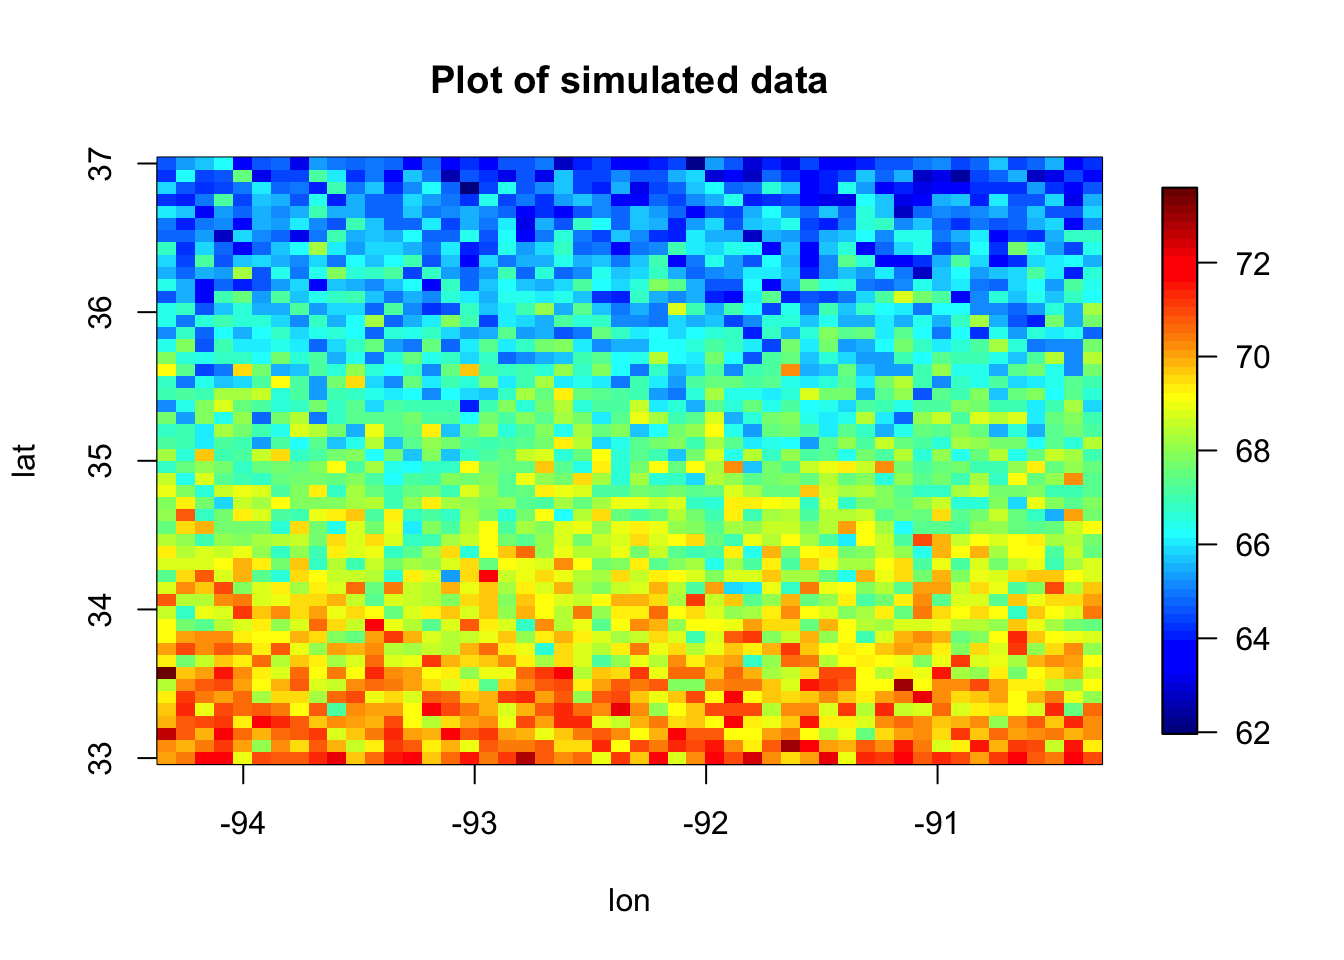
\includegraphics{STAT-5413_files/figure-latex/unnamed-chunk-20-1.pdf}

\begin{Shaded}
\begin{Highlighting}[]
\KeywordTok{contour}\NormalTok{(lon, lat, y, }\DataTypeTok{main =} \StringTok{"Contour plot of simulated data"}\NormalTok{)}
\end{Highlighting}
\end{Shaded}

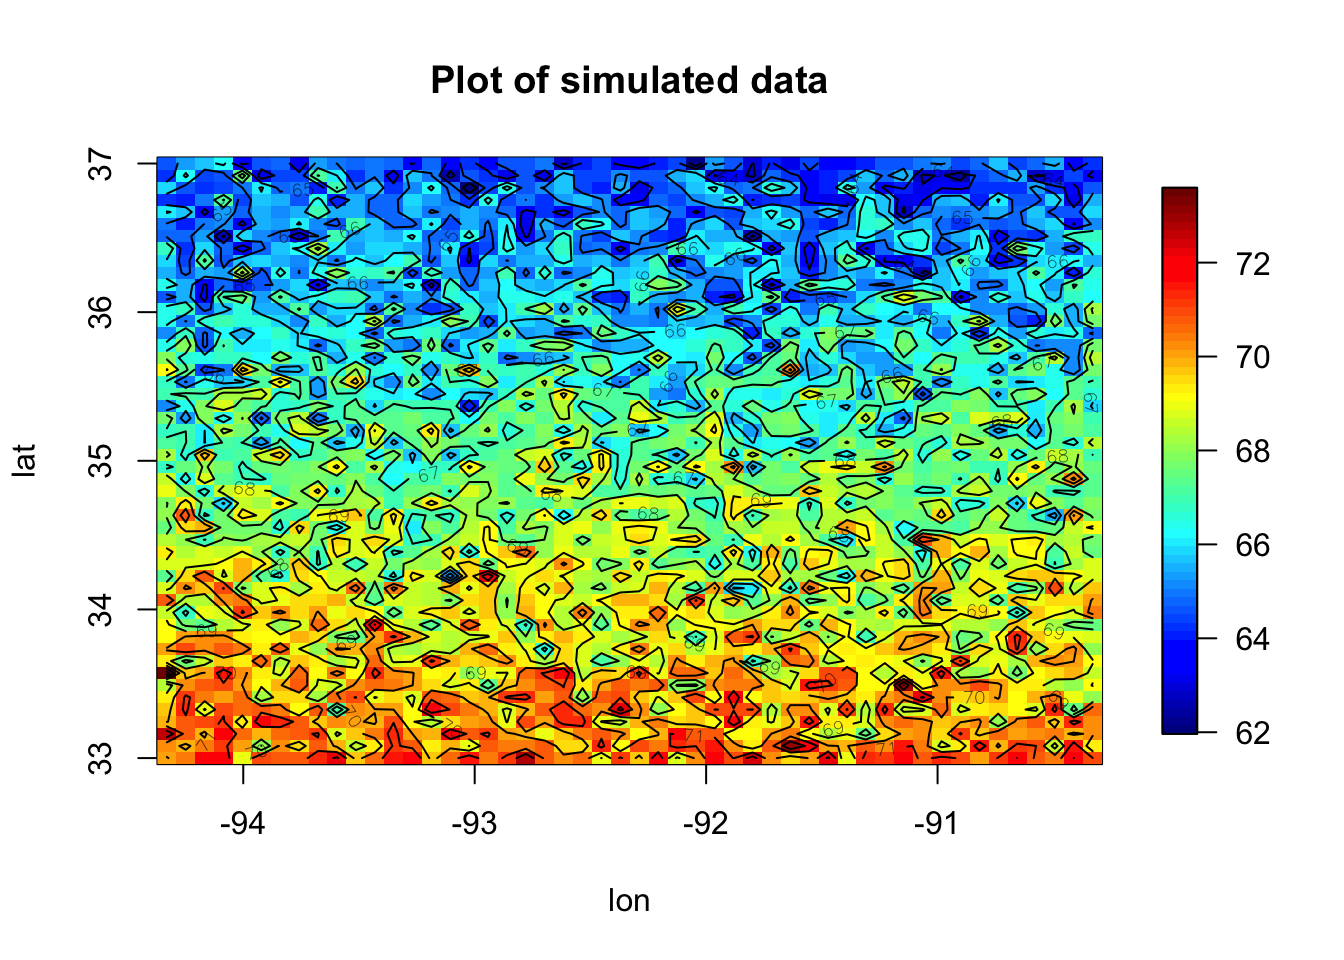
\includegraphics{STAT-5413_files/figure-latex/unnamed-chunk-21-1.pdf}

\begin{Shaded}
\begin{Highlighting}[]
\KeywordTok{image.plot}\NormalTok{(lon, lat, y, }\DataTypeTok{main =} \StringTok{"Plot of simulated data"}\NormalTok{)}
\KeywordTok{contour}\NormalTok{(lon, lat, y, }\DataTypeTok{main =} \StringTok{"Contour plot of simulated data"}\NormalTok{, }\DataTypeTok{add =} \OtherTok{TRUE}\NormalTok{,}
        \DataTypeTok{nlevels =} \DecValTok{10}\NormalTok{)}
\end{Highlighting}
\end{Shaded}

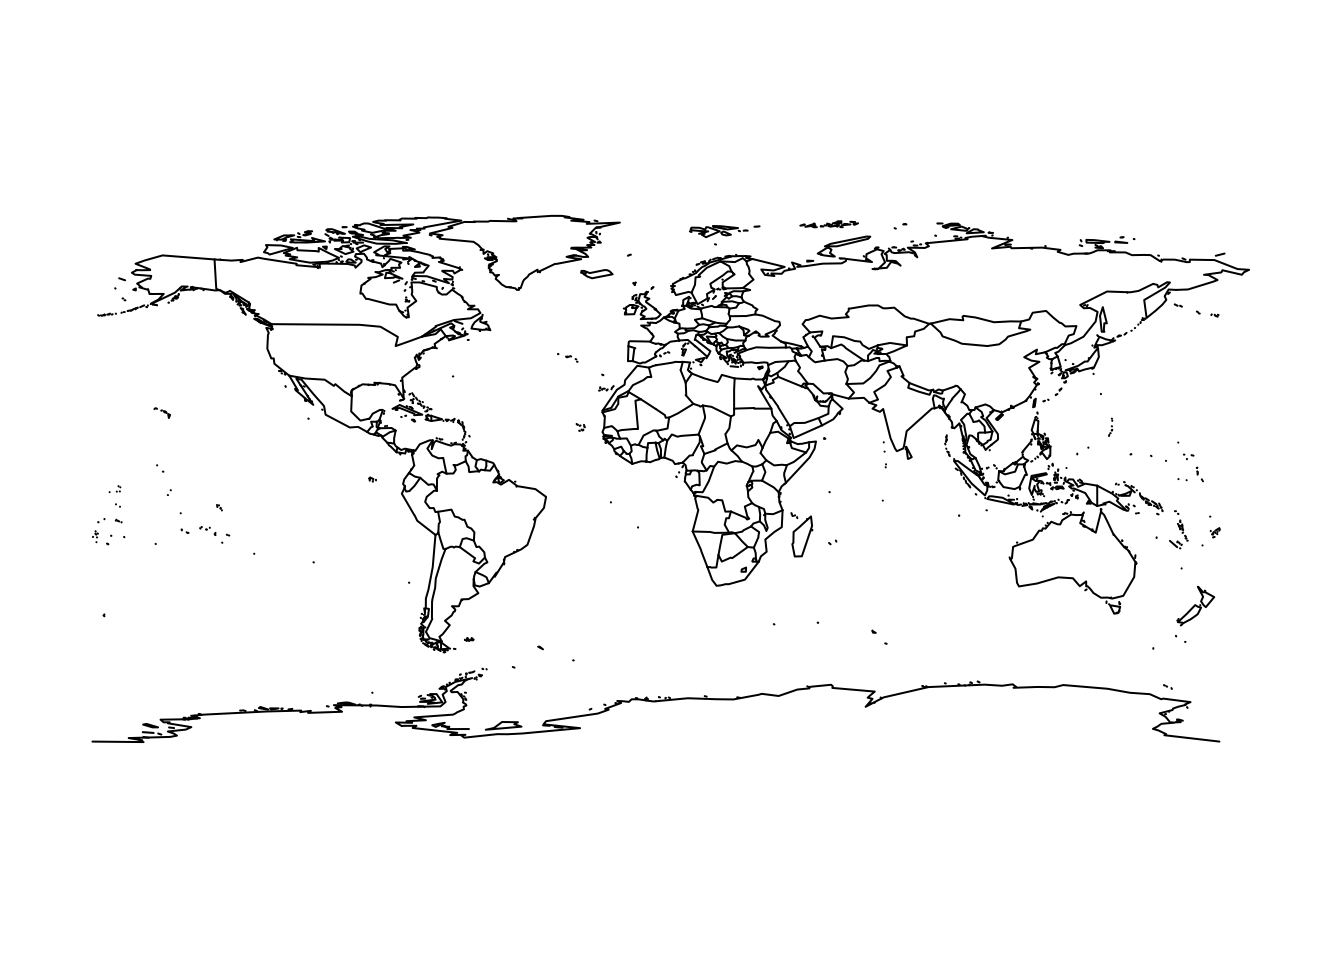
\includegraphics{STAT-5413_files/figure-latex/unnamed-chunk-22-1.pdf}

\begin{Shaded}
\begin{Highlighting}[]
\CommentTok{## adding in maps}
\KeywordTok{library}\NormalTok{(maps)}
\NormalTok{maps}\OperatorTok{::}\KeywordTok{map}\NormalTok{(}\StringTok{"world"}\NormalTok{)}
\end{Highlighting}
\end{Shaded}

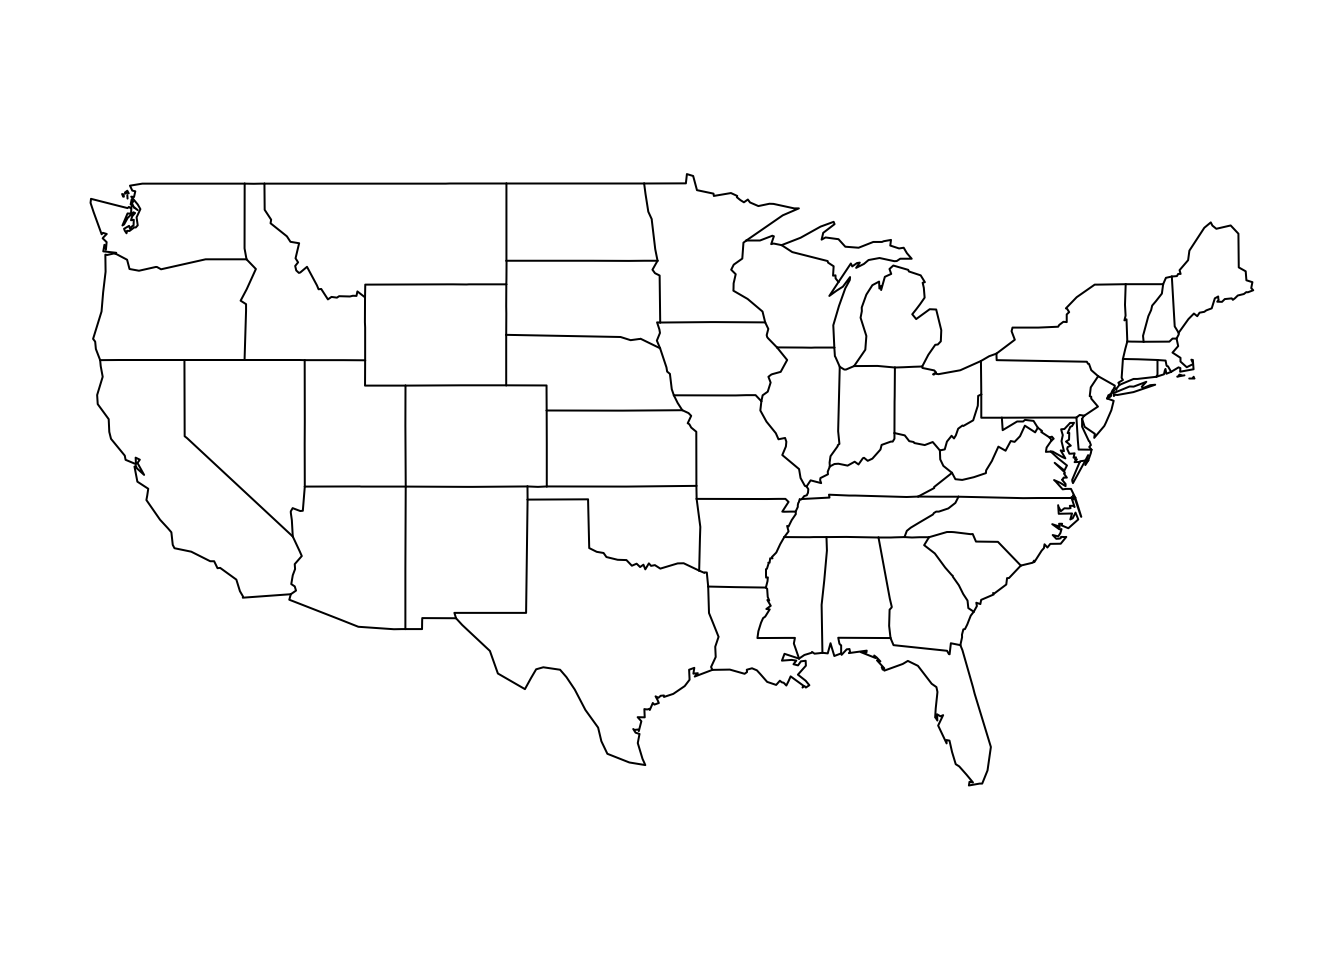
\includegraphics{STAT-5413_files/figure-latex/unnamed-chunk-23-1.pdf}

\begin{Shaded}
\begin{Highlighting}[]
\NormalTok{maps}\OperatorTok{::}\KeywordTok{map}\NormalTok{(}\StringTok{"state"}\NormalTok{)}
\end{Highlighting}
\end{Shaded}

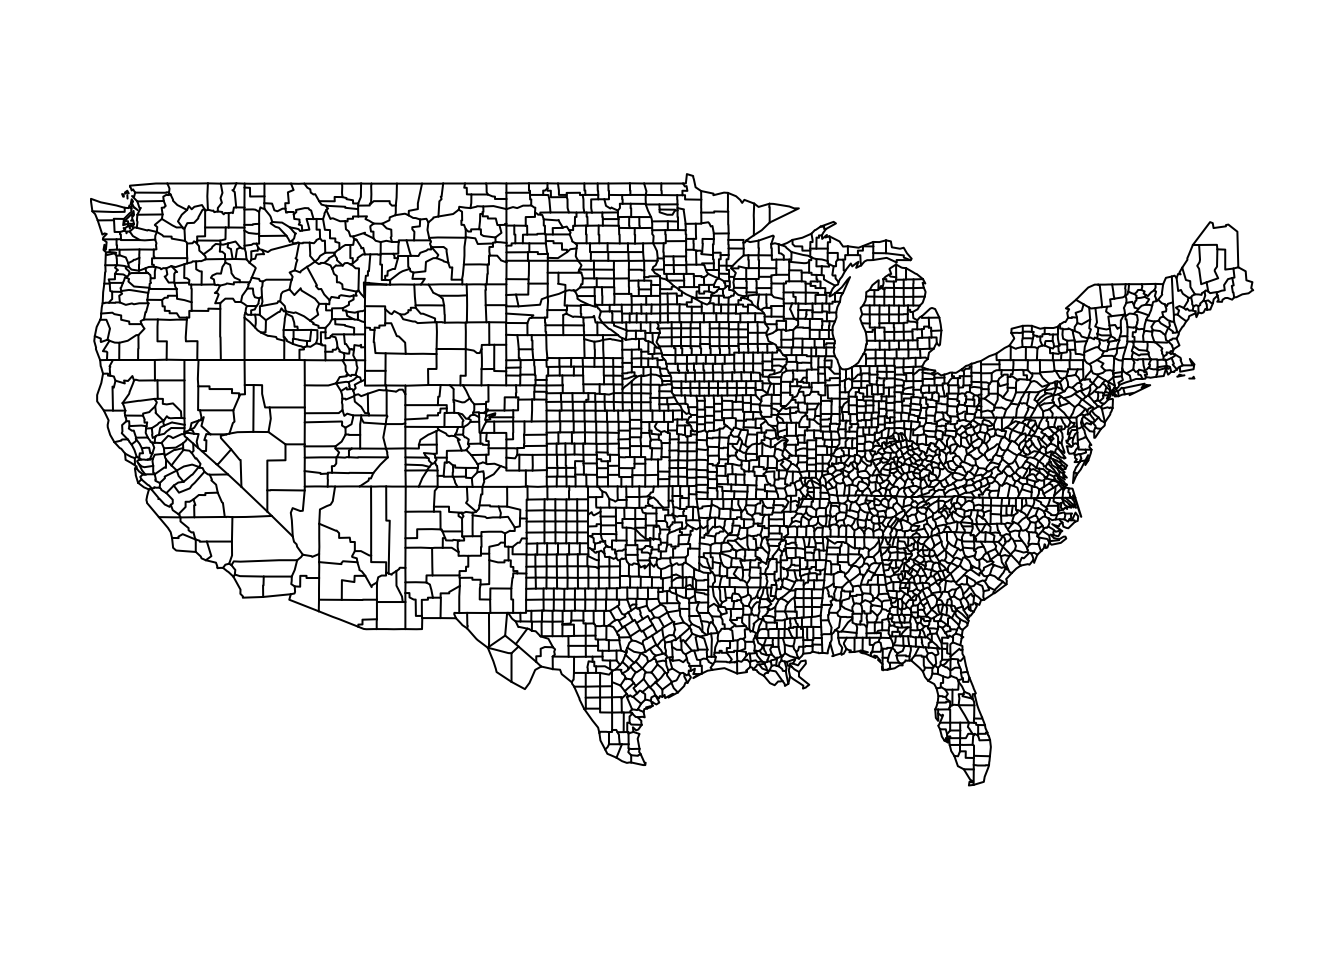
\includegraphics{STAT-5413_files/figure-latex/unnamed-chunk-24-1.pdf}

\begin{Shaded}
\begin{Highlighting}[]
\NormalTok{maps}\OperatorTok{::}\KeywordTok{map}\NormalTok{(}\StringTok{"county"}\NormalTok{)}
\end{Highlighting}
\end{Shaded}

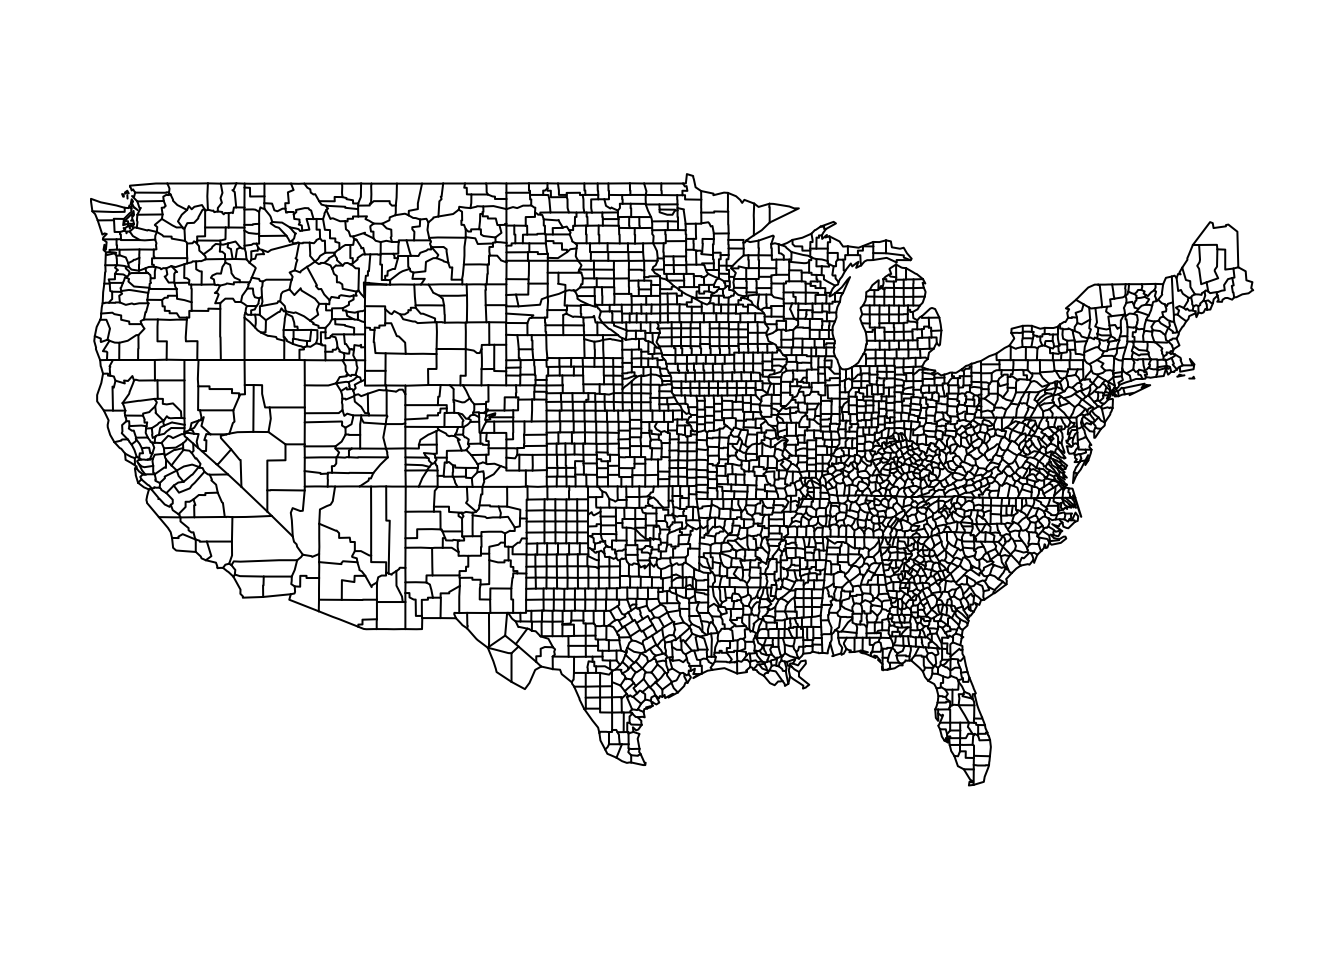
\includegraphics{STAT-5413_files/figure-latex/unnamed-chunk-25-1.pdf}

\begin{Shaded}
\begin{Highlighting}[]
\NormalTok{maps}\OperatorTok{::}\KeywordTok{map}\NormalTok{(}\StringTok{"county"}\NormalTok{, }\StringTok{"Arkansas"}\NormalTok{)}
\KeywordTok{points}\NormalTok{(s, }\DataTypeTok{cex =} \FloatTok{0.3}\NormalTok{)}
\end{Highlighting}
\end{Shaded}

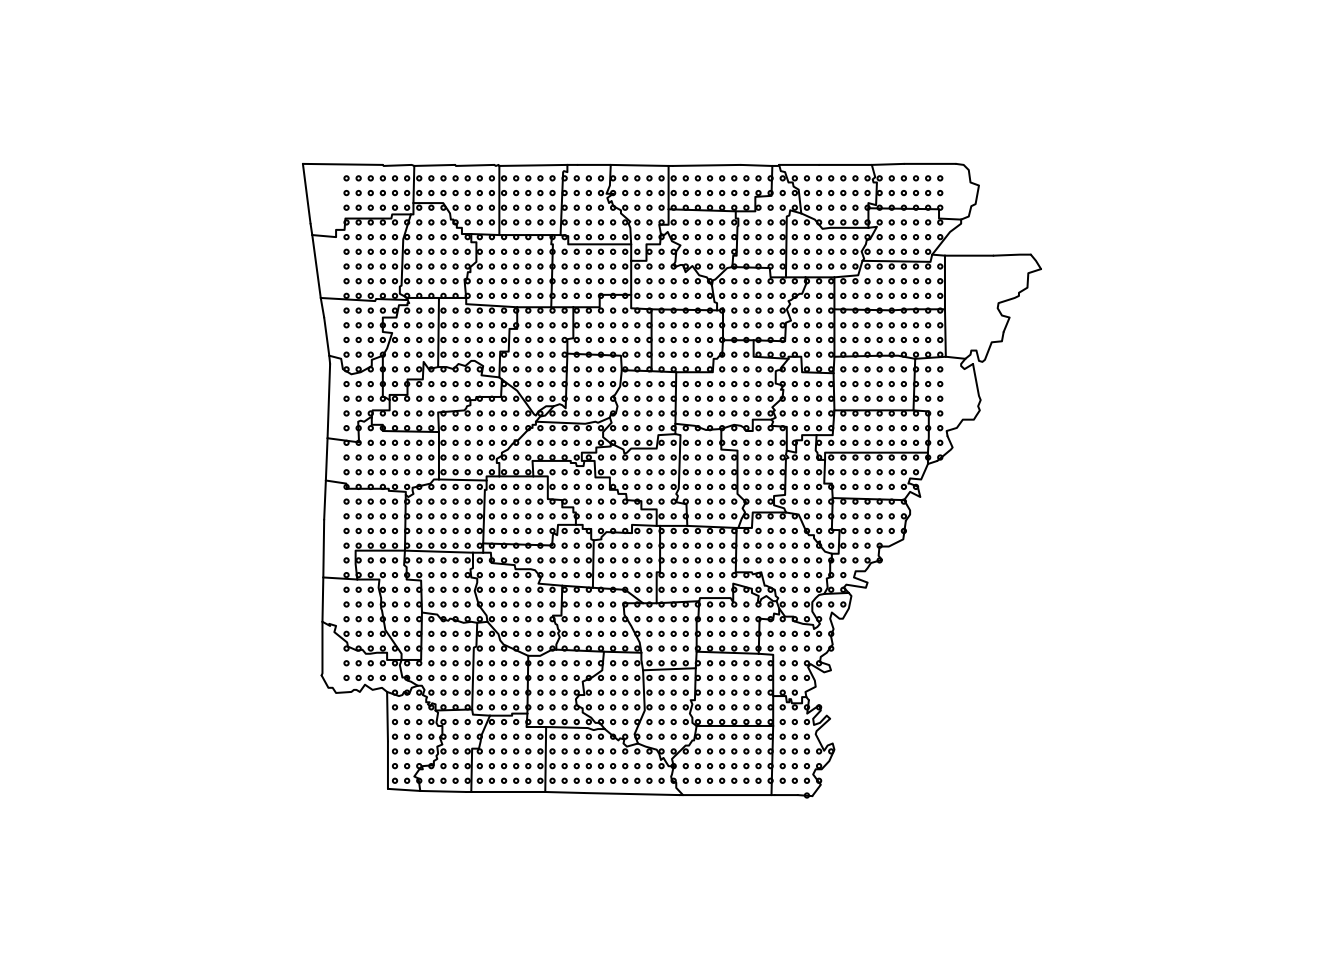
\includegraphics{STAT-5413_files/figure-latex/unnamed-chunk-26-1.pdf}

\begin{Shaded}
\begin{Highlighting}[]
\NormalTok{state <-}\StringTok{ }\KeywordTok{map.where}\NormalTok{(}\StringTok{"state"}\NormalTok{, }\DataTypeTok{x =}\NormalTok{ s[, }\DecValTok{1}\NormalTok{], }\DataTypeTok{y =}\NormalTok{ s[, }\DecValTok{2}\NormalTok{])}
\KeywordTok{head}\NormalTok{(state)}
\end{Highlighting}
\end{Shaded}

\begin{verbatim}
## [1] "texas"     "texas"     "texas"     "texas"     "louisiana" "louisiana"
\end{verbatim}

\begin{Shaded}
\begin{Highlighting}[]
\KeywordTok{table}\NormalTok{(state)}
\end{Highlighting}
\end{Shaded}

\begin{verbatim}
## state
##    arkansas   louisiana mississippi    missouri       texas 
##        1903          34         180         351          32
\end{verbatim}

\begin{Shaded}
\begin{Highlighting}[]
\CommentTok{## subset only points in arkansas}
\NormalTok{dat <-}\StringTok{ }\KeywordTok{data.frame}\NormalTok{(}
    \DataTypeTok{lon   =}\NormalTok{ s[, }\DecValTok{1}\NormalTok{],}
    \DataTypeTok{lat   =}\NormalTok{ s[, }\DecValTok{2}\NormalTok{],}
    \DataTypeTok{state =}\NormalTok{ state}
\NormalTok{)}

\NormalTok{maps}\OperatorTok{::}\KeywordTok{map}\NormalTok{(}\StringTok{"county"}\NormalTok{, }\StringTok{"Arkansas"}\NormalTok{)}
\NormalTok{dat }\OperatorTok\StringTok{ }
\StringTok{    }\KeywordTok{subset}\NormalTok{(state }\OperatorTok{==}\StringTok{ "arkansas"}\NormalTok{) }\OperatorTok
\StringTok{    }\KeywordTok{points}\NormalTok{(}\DataTypeTok{cex =} \FloatTok{0.3}\NormalTok{)}
\end{Highlighting}
\end{Shaded}

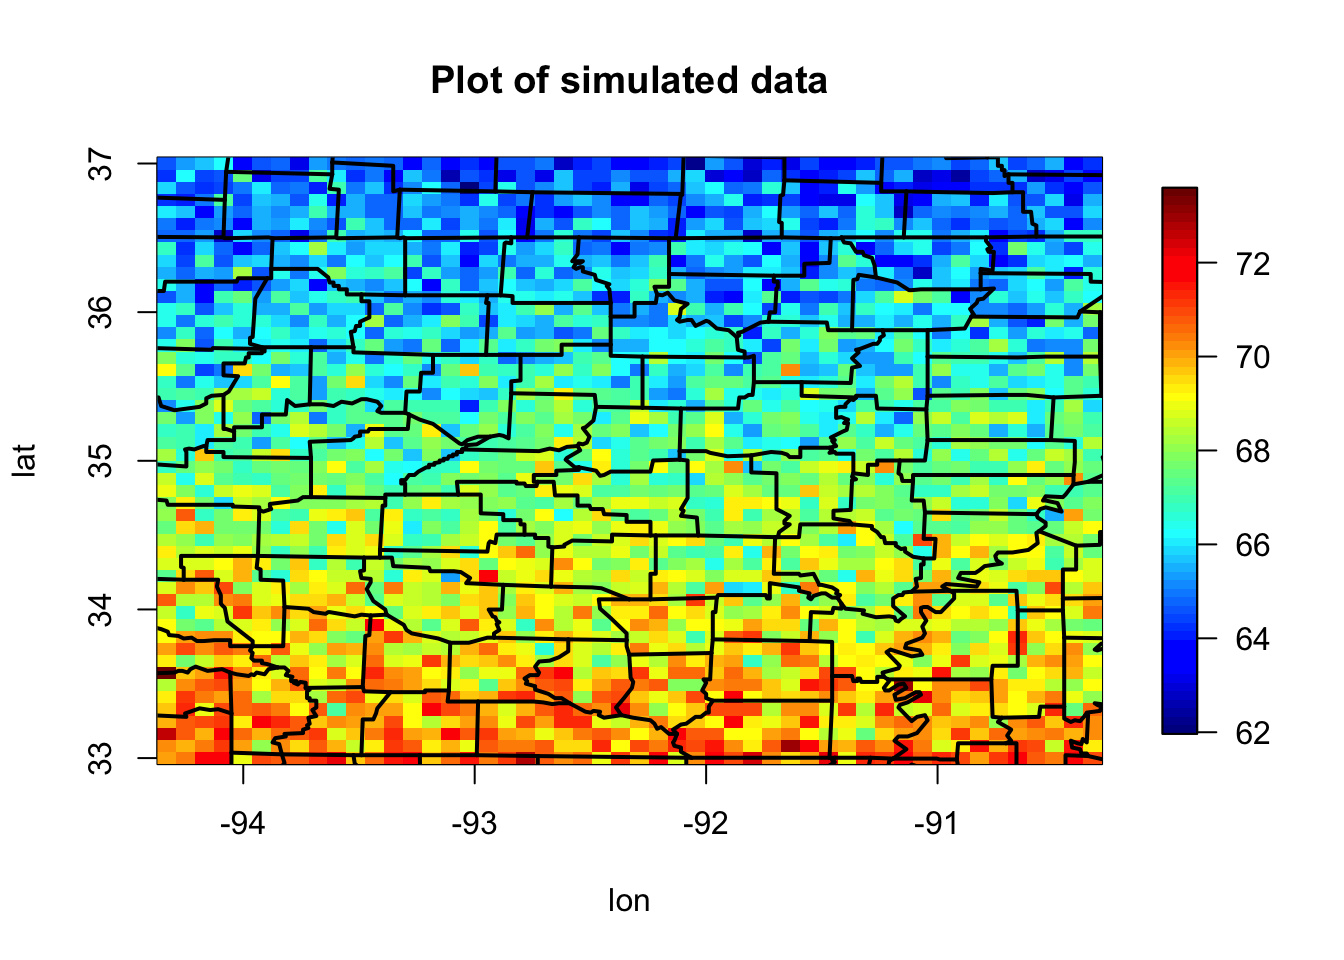
\includegraphics{STAT-5413_files/figure-latex/unnamed-chunk-27-1.pdf}

Plot the simulated data with the county boundaries

\begin{Shaded}
\begin{Highlighting}[]
\KeywordTok{image.plot}\NormalTok{(lon, lat, y, }\DataTypeTok{main =} \StringTok{"Plot of simulated data"}\NormalTok{)}
\NormalTok{maps}\OperatorTok{::}\KeywordTok{map}\NormalTok{(}\StringTok{"county"}\NormalTok{, }\DataTypeTok{add =} \OtherTok{TRUE}\NormalTok{, }\DataTypeTok{lwd =} \DecValTok{2}\NormalTok{)}
\end{Highlighting}
\end{Shaded}

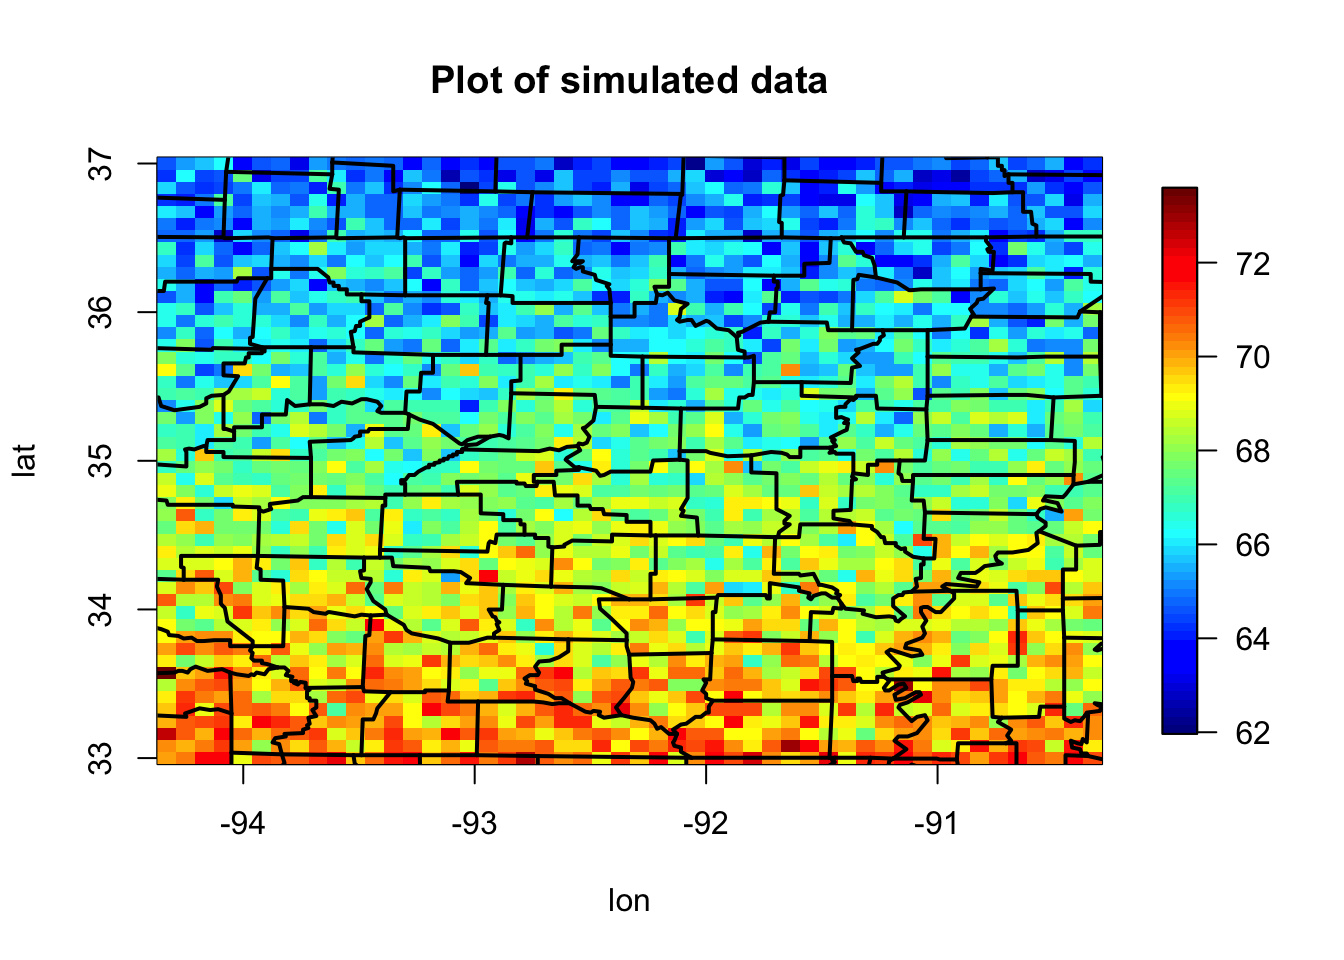
\includegraphics{STAT-5413_files/figure-latex/unnamed-chunk-28-1.pdf}

\begin{Shaded}
\begin{Highlighting}[]
\CommentTok{## change the aspect ratio}
\KeywordTok{image.plot}\NormalTok{(lon, lat, y, }\DataTypeTok{main =} \StringTok{"Plot of simulated data"}\NormalTok{, }\DataTypeTok{asp =} \FloatTok{1.3}\NormalTok{)}
\NormalTok{maps}\OperatorTok{::}\KeywordTok{map}\NormalTok{(}\StringTok{"county"}\NormalTok{, }\DataTypeTok{add =} \OtherTok{TRUE}\NormalTok{, }\DataTypeTok{lwd =} \DecValTok{2}\NormalTok{)}
\end{Highlighting}
\end{Shaded}

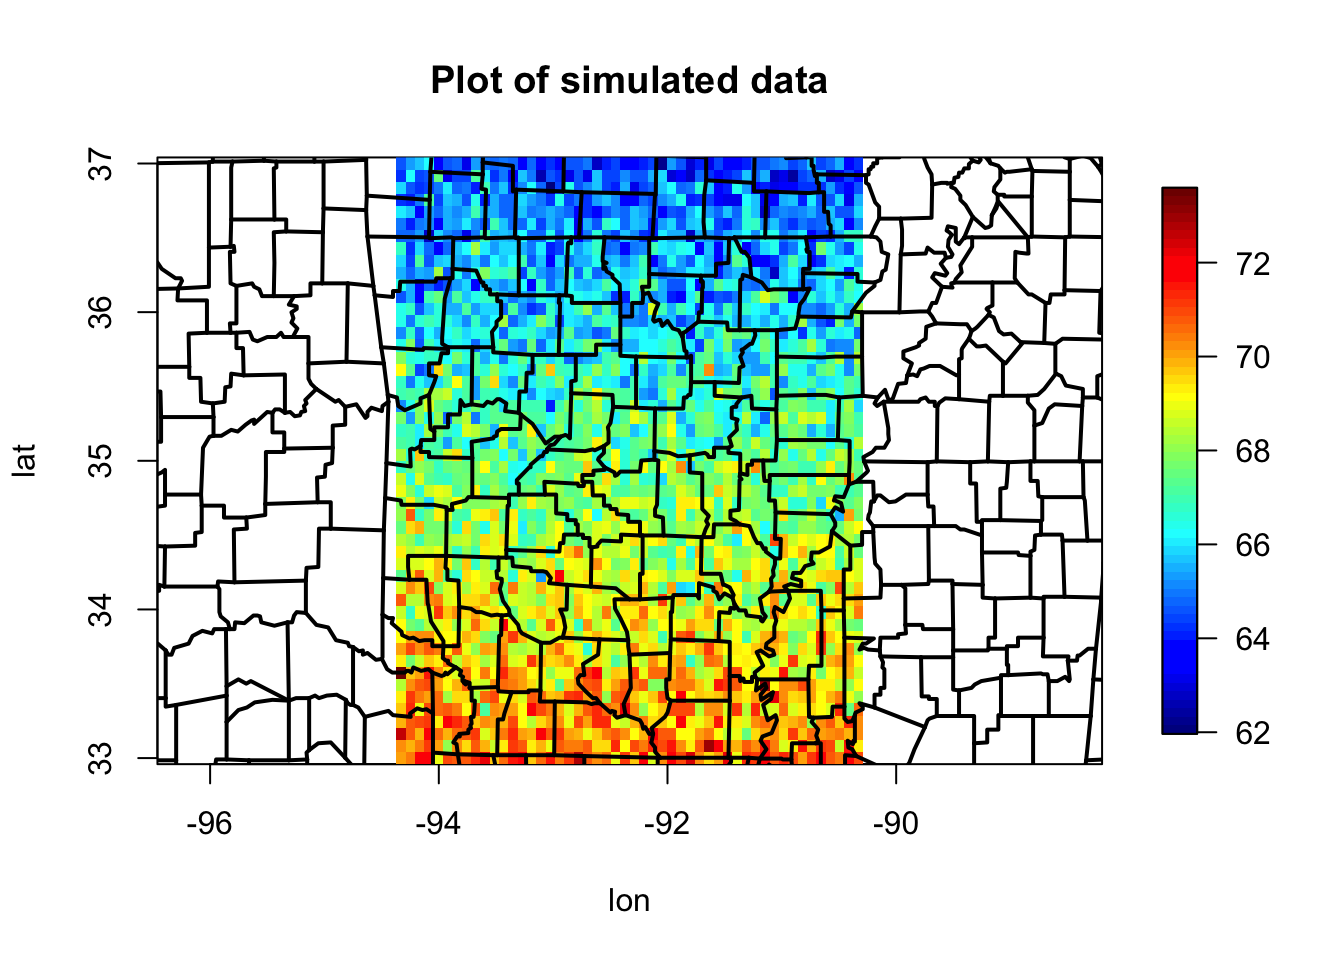
\includegraphics{STAT-5413_files/figure-latex/unnamed-chunk-29-1.pdf}

\hypertarget{spatial-visualization-using-fields-1}{%
\subsection{\texorpdfstring{Spatial visualization using \emph{fields}}{Spatial visualization using fields}}\label{spatial-visualization-using-fields-1}}

\begin{Shaded}
\begin{Highlighting}[]
\NormalTok{nx <-}\StringTok{ }\DecValTok{100}
\NormalTok{ny <-}\StringTok{ }\DecValTok{100}

\KeywordTok{library}\NormalTok{(maps)  }\CommentTok{# for map.where}

\CommentTok{# Corner of the USA}
\NormalTok{corners <-}\StringTok{ }\KeywordTok{c}\NormalTok{(}\OperatorTok{-}\FloatTok{124.733056}\NormalTok{, }\FloatTok{-66.947028}\NormalTok{, }\FloatTok{24.520833}\NormalTok{, }\FloatTok{49.384472}\NormalTok{)}

\CommentTok{# create grid}
\NormalTok{grid <-}\StringTok{ }\KeywordTok{expand.grid}\NormalTok{(}
    \KeywordTok{seq}\NormalTok{(corners[}\DecValTok{1}\NormalTok{], corners[}\DecValTok{2}\NormalTok{], }\DataTypeTok{length =}\NormalTok{ nx), }
    \KeywordTok{seq}\NormalTok{(corners[}\DecValTok{3}\NormalTok{], corners[}\DecValTok{4}\NormalTok{], }\DataTypeTok{length =}\NormalTok{ ny)}
\NormalTok{)}

\NormalTok{dat <-}\StringTok{ }\KeywordTok{data.frame}\NormalTok{(}
    \DataTypeTok{lon  =}\NormalTok{ grid[, }\DecValTok{1}\NormalTok{],}
    \DataTypeTok{lat  =}\NormalTok{ grid[, }\DecValTok{2}\NormalTok{],}
    \DataTypeTok{inUS =} \KeywordTok{ifelse}\NormalTok{(}\KeywordTok{is.na}\NormalTok{(}\KeywordTok{map.where}\NormalTok{(}\StringTok{"usa"}\NormalTok{, }\DataTypeTok{x =}\NormalTok{ grid[, }\DecValTok{1}\NormalTok{], }\DataTypeTok{y =}\NormalTok{ grid[, }\DecValTok{2}\NormalTok{])), }\OtherTok{FALSE}\NormalTok{, }\OtherTok{TRUE}\NormalTok{)}
\NormalTok{)}

\CommentTok{## Plot only points in the us}

\NormalTok{dat }\OperatorTok
\StringTok{    }\KeywordTok{subset}\NormalTok{(inUS) }\OperatorTok\StringTok{   }\CommentTok{## this selects only the true values}
\StringTok{    }\KeywordTok{ggplot}\NormalTok{(}\KeywordTok{aes}\NormalTok{(}\DataTypeTok{x =}\NormalTok{ lon, }\DataTypeTok{y =}\NormalTok{ lat)) }\OperatorTok{+}
\StringTok{    }\KeywordTok{geom_point}\NormalTok{(}\DataTypeTok{size =} \FloatTok{0.6}\NormalTok{, }\DataTypeTok{alpha =} \FloatTok{0.5}\NormalTok{)}
\end{Highlighting}
\end{Shaded}

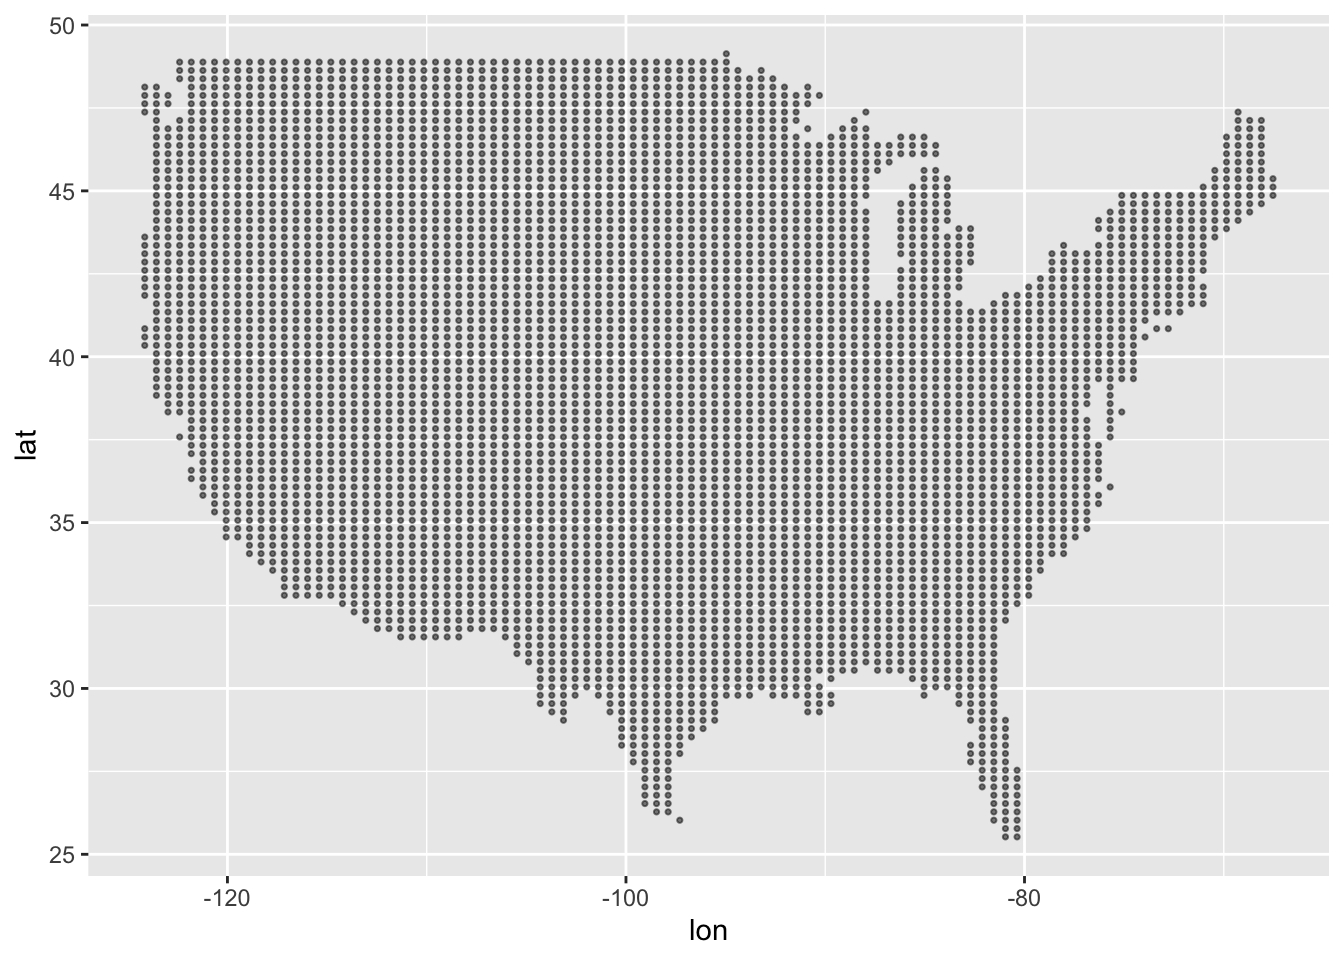
\includegraphics{STAT-5413_files/figure-latex/unnamed-chunk-30-1.pdf}

\begin{Shaded}
\begin{Highlighting}[]
\CommentTok{## Simulate some data over the grid}
\NormalTok{dat}\OperatorTok{$}\NormalTok{y <-}\StringTok{ }\KeywordTok{sin}\NormalTok{(}\DecValTok{2} \OperatorTok{*}\StringTok{ }\NormalTok{pi }\OperatorTok{*}\StringTok{ }\NormalTok{dat}\OperatorTok{$}\NormalTok{lon }\OperatorTok{/}\StringTok{ }\DecValTok{10}\NormalTok{) }\OperatorTok{+}\StringTok{ }\KeywordTok{cos}\NormalTok{(}\DecValTok{2} \OperatorTok{*}\NormalTok{pi }\OperatorTok{*}\StringTok{ }\NormalTok{dat}\OperatorTok{$}\NormalTok{lat }\OperatorTok{/}\StringTok{ }\DecValTok{10}\NormalTok{) }\OperatorTok{+}
\StringTok{    }\KeywordTok{sin}\NormalTok{(}\DecValTok{2} \OperatorTok{*}\StringTok{ }\NormalTok{pi }\OperatorTok{*}\StringTok{ }\NormalTok{dat}\OperatorTok{$}\NormalTok{lon }\OperatorTok{/}\StringTok{ }\DecValTok{10}\NormalTok{) }\OperatorTok{*}\StringTok{ }\KeywordTok{cos}\NormalTok{(}\DecValTok{2} \OperatorTok{*}\NormalTok{pi }\OperatorTok{*}\StringTok{ }\NormalTok{dat}\OperatorTok{$}\NormalTok{lat }\OperatorTok{/}\StringTok{ }\DecValTok{10}\NormalTok{)}

\CommentTok{## plot each of the responses grouped by latitude}
\NormalTok{dat }\OperatorTok
\StringTok{    }\KeywordTok{ggplot}\NormalTok{(}\KeywordTok{aes}\NormalTok{(}\DataTypeTok{x =}\NormalTok{ lon, }\DataTypeTok{y =}\NormalTok{ y, }\DataTypeTok{group =}\NormalTok{ lat, }\DataTypeTok{color =}\NormalTok{ lat)) }\OperatorTok{+}
\StringTok{    }\KeywordTok{geom_line}\NormalTok{()}
\end{Highlighting}
\end{Shaded}

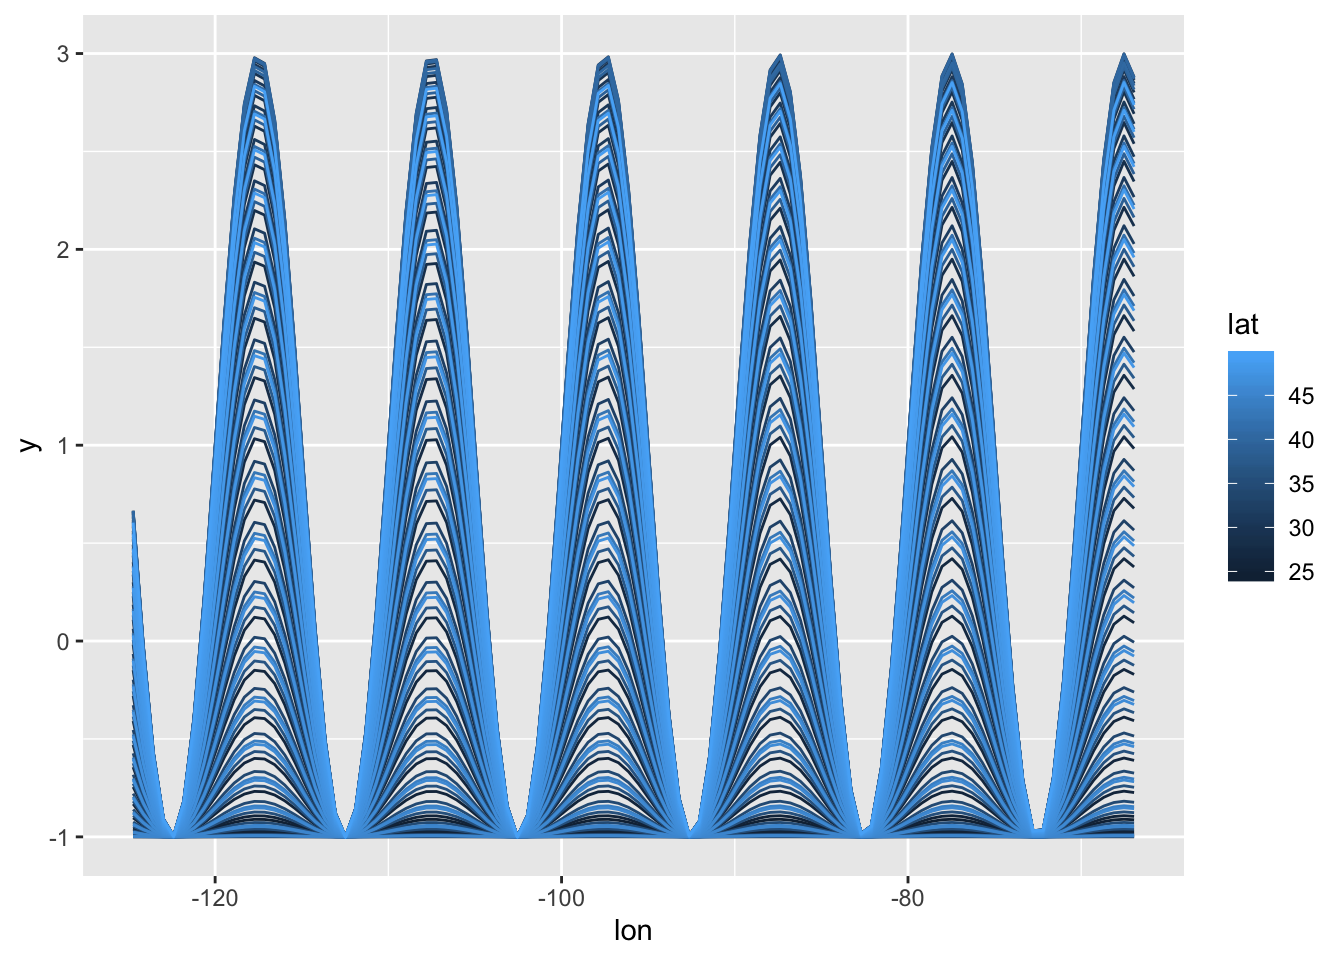
\includegraphics{STAT-5413_files/figure-latex/unnamed-chunk-30-2.pdf}

\begin{Shaded}
\begin{Highlighting}[]
\CommentTok{## Function to generate maps}
\NormalTok{map_points <-}\StringTok{ }\ControlFlowTok{function}\NormalTok{ (dat,}
                        \DataTypeTok{color_low =} \StringTok{"white"}\NormalTok{, }\DataTypeTok{color_high =} \StringTok{"darkred"}\NormalTok{, }
                        \DataTypeTok{color_na =} \KeywordTok{gray}\NormalTok{(}\FloatTok{0.9}\NormalTok{), }\DataTypeTok{zeroiswhite =} \OtherTok{FALSE}\NormalTok{,}
                        \DataTypeTok{xlim =} \OtherTok{NULL}\NormalTok{, }\DataTypeTok{ylim =} \OtherTok{NULL}\NormalTok{, }\DataTypeTok{zlim =} \OtherTok{NULL}\NormalTok{,}
                        \DataTypeTok{mainTitle =} \OtherTok{NULL}\NormalTok{, }\DataTypeTok{legendTitle =} \StringTok{""}\NormalTok{) \{}
    \KeywordTok{library}\NormalTok{(ggplot2)}
    
    \CommentTok{## check if the data.fram dat contains the correct variables}
    \ControlFlowTok{if}\NormalTok{ (}\KeywordTok{is.null}\NormalTok{(dat}\OperatorTok{$}\NormalTok{lon)) \{ }\KeywordTok{stop}\NormalTok{(}\StringTok{'The data.frame dat must contain a "lon" variable'}\NormalTok{) \}}
    \ControlFlowTok{if}\NormalTok{ (}\KeywordTok{is.null}\NormalTok{(dat}\OperatorTok{$}\NormalTok{lat)) \{ }\KeywordTok{stop}\NormalTok{(}\StringTok{'The data.frame dat must contain a "lat" variable'}\NormalTok{) \}}
    \ControlFlowTok{if}\NormalTok{ (}\KeywordTok{is.null}\NormalTok{(dat}\OperatorTok{$}\NormalTok{y))   \{ }\KeywordTok{stop}\NormalTok{(}\StringTok{'The data.frame dat must contain a "y" variable'}\NormalTok{) \}}
    
    \CommentTok{# Store the base data of the underlying map}
\NormalTok{    states <-}\StringTok{ }\KeywordTok{map_data}\NormalTok{(}\StringTok{"state"}\NormalTok{)}
    
    \CommentTok{# Set limits for x, y, z if not specified as parameters}
    \ControlFlowTok{if}\NormalTok{ (}\KeywordTok{is.null}\NormalTok{(xlim)) \{ xlim <-}\StringTok{ }\KeywordTok{range}\NormalTok{(dat}\OperatorTok{$}\NormalTok{lon, }\DataTypeTok{na.rm =} \OtherTok{TRUE}\NormalTok{) \}}
    \ControlFlowTok{if}\NormalTok{ (}\KeywordTok{is.null}\NormalTok{(ylim)) \{ ylim <-}\StringTok{ }\KeywordTok{range}\NormalTok{(dat}\OperatorTok{$}\NormalTok{lat, }\DataTypeTok{na.rm =} \OtherTok{TRUE}\NormalTok{) \}}
    \ControlFlowTok{if}\NormalTok{ (}\KeywordTok{is.null}\NormalTok{(zlim)) \{ zlim <-}\StringTok{ }\KeywordTok{range}\NormalTok{(dat}\OperatorTok{$}\NormalTok{y, }\DataTypeTok{na.rm =} \OtherTok{TRUE}\NormalTok{) \}}
    
    \CommentTok{# Create the plot}
\NormalTok{    p <-}\StringTok{ }\KeywordTok{ggplot}\NormalTok{(dat, }\KeywordTok{aes}\NormalTok{(}\DataTypeTok{x =}\NormalTok{ lon, }\DataTypeTok{y =}\NormalTok{ lat)) }\OperatorTok{+}
\StringTok{        }\KeywordTok{theme_bw}\NormalTok{()}
\NormalTok{    p <-}\StringTok{ }\NormalTok{p }\OperatorTok{+}\StringTok{ }\KeywordTok{theme}\NormalTok{(}\DataTypeTok{plot.title =} \KeywordTok{element_text}\NormalTok{(}\DataTypeTok{size =} \KeywordTok{rel}\NormalTok{(}\FloatTok{1.5}\NormalTok{)))}
\NormalTok{    p <-}\StringTok{ }\NormalTok{p }\OperatorTok{+}\StringTok{ }\KeywordTok{geom_point}\NormalTok{(}\KeywordTok{aes}\NormalTok{(}\DataTypeTok{colour =}\NormalTok{ y))}
    \CommentTok{## add in the map}
\NormalTok{    p <-}\StringTok{ }\NormalTok{p }\OperatorTok{+}\StringTok{ }\KeywordTok{geom_polygon}\NormalTok{(}\DataTypeTok{data =}\NormalTok{ states, }\KeywordTok{aes}\NormalTok{(}\DataTypeTok{x =}\NormalTok{ long, }\DataTypeTok{y =}\NormalTok{ lat, }\DataTypeTok{group =}\NormalTok{ group), }
                          \DataTypeTok{colour =} \StringTok{"black"}\NormalTok{, }\DataTypeTok{fill =} \OtherTok{NA}\NormalTok{) }
    \CommentTok{## a 1.3 coordinate ratio is visually appealing}
\NormalTok{    p <-}\StringTok{ }\NormalTok{p }\OperatorTok{+}\StringTok{ }\KeywordTok{coord_fixed}\NormalTok{(}\DataTypeTok{ratio =} \FloatTok{1.3}\NormalTok{, }\DataTypeTok{xlim =}\NormalTok{ xlim, }\DataTypeTok{ylim =}\NormalTok{ ylim)}
\NormalTok{    p <-}\StringTok{ }\NormalTok{p }\OperatorTok{+}\StringTok{ }\KeywordTok{labs}\NormalTok{(}\DataTypeTok{title =} \KeywordTok{paste}\NormalTok{(mainTitle, }\StringTok{"}\CharTok{\textbackslash{}n}\StringTok{"}\NormalTok{, }\DataTypeTok{sep=}\StringTok{""}\NormalTok{), }\DataTypeTok{x =} \StringTok{""}\NormalTok{, }\DataTypeTok{y =} \StringTok{""}\NormalTok{)}
    \ControlFlowTok{if}\NormalTok{(zeroiswhite)\{}
\NormalTok{        p <-}\StringTok{ }\NormalTok{p }\OperatorTok{+}\StringTok{ }\KeywordTok{scale_colour_gradient2}\NormalTok{(}
            \DataTypeTok{low      =}\NormalTok{  color_low, }
            \DataTypeTok{high     =}\NormalTok{ color_high,}
            \DataTypeTok{na.value =}\NormalTok{ color_na,}
            \DataTypeTok{limits   =}\NormalTok{ zlim,}
            \DataTypeTok{name     =}\NormalTok{ legendTitle}
\NormalTok{        ) }
\NormalTok{    \}}
    \ControlFlowTok{if}\NormalTok{(}\OperatorTok{!}\NormalTok{zeroiswhite)\{}
\NormalTok{        p <-}\StringTok{ }\NormalTok{p }\OperatorTok{+}\StringTok{ }\KeywordTok{scale_colour_gradient}\NormalTok{(}
            \DataTypeTok{low      =}\NormalTok{ color_low, }
            \DataTypeTok{high     =}\NormalTok{ color_high,}
            \DataTypeTok{na.value =}\NormalTok{ color_na,}
            \DataTypeTok{limits   =}\NormalTok{ zlim,}
            \DataTypeTok{name     =}\NormalTok{ legendTitle}
\NormalTok{        ) }
\NormalTok{    \}}
    \KeywordTok{return}\NormalTok{(p)  }
\NormalTok{\}}
\end{Highlighting}
\end{Shaded}

\begin{Shaded}
\begin{Highlighting}[]
\CommentTok{## Let's make some plots}
\NormalTok{dat }\OperatorTok
\StringTok{    }\KeywordTok{map_points}\NormalTok{(}
        \DataTypeTok{color_low  =} \StringTok{"pink"}\NormalTok{, }
        \DataTypeTok{color_high =} \StringTok{"black"}\NormalTok{,}
        \DataTypeTok{mainTitle  =} \StringTok{"Entire United States"}
\NormalTok{    )}
\end{Highlighting}
\end{Shaded}

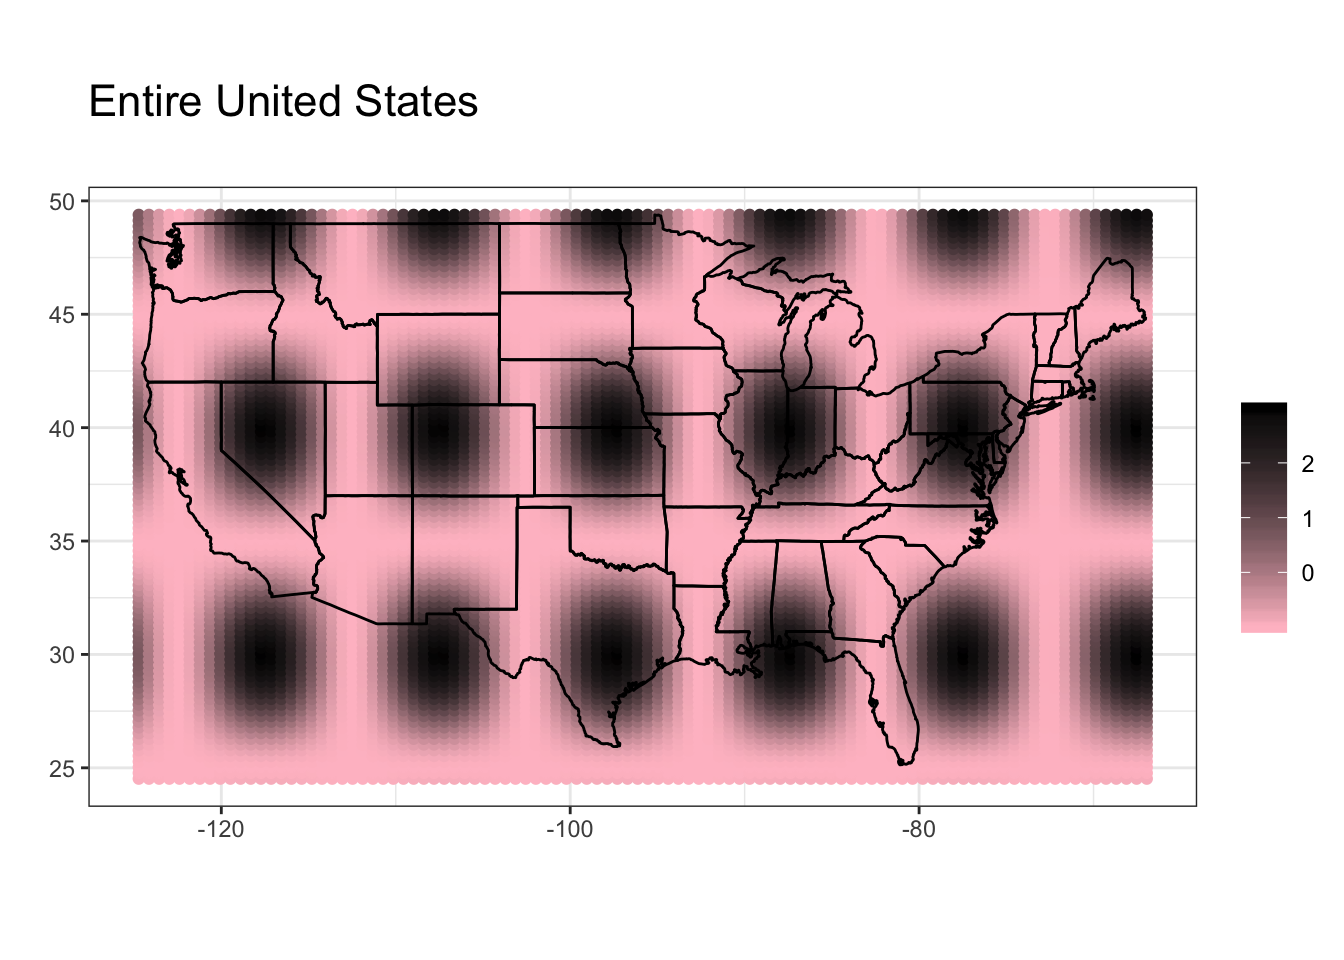
\includegraphics{STAT-5413_files/figure-latex/unnamed-chunk-32-1.pdf}

\begin{Shaded}
\begin{Highlighting}[]
\CommentTok{## Subset only the US}
\NormalTok{dat }\OperatorTok
\StringTok{    }\KeywordTok{subset}\NormalTok{(inUS) }\OperatorTok
\StringTok{    }\KeywordTok{map_points}\NormalTok{(}
        \DataTypeTok{color_low  =} \StringTok{"pink"}\NormalTok{, }
        \DataTypeTok{color_high =} \StringTok{"black"}\NormalTok{,}
        \DataTypeTok{mainTitle  =} \StringTok{"Entire United States"}
\NormalTok{    )}
\end{Highlighting}
\end{Shaded}

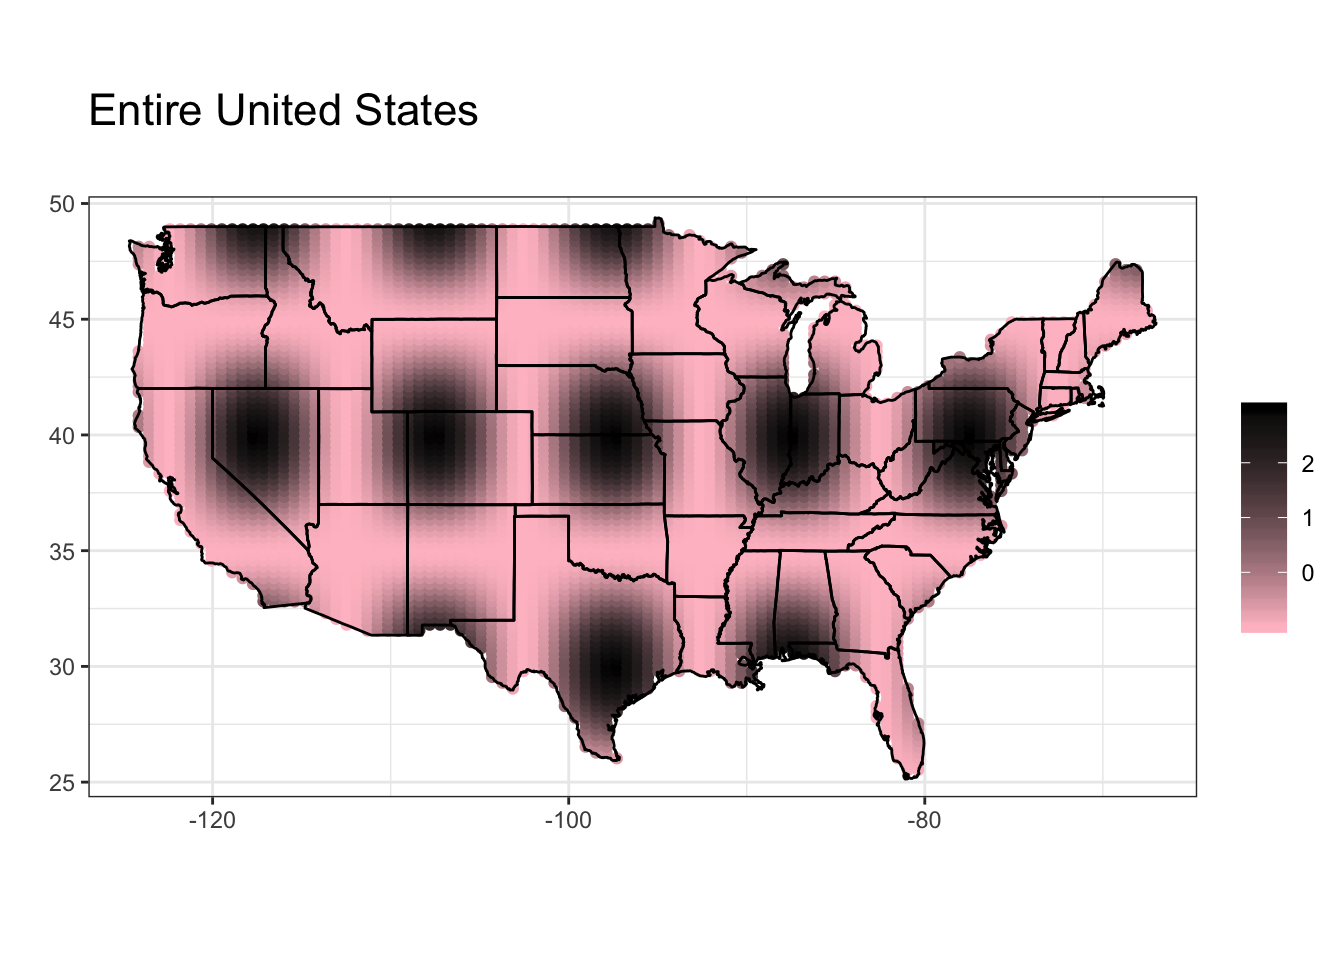
\includegraphics{STAT-5413_files/figure-latex/unnamed-chunk-32-2.pdf}

\begin{Shaded}
\begin{Highlighting}[]
\CommentTok{## plot only a subset of points}
\NormalTok{dat }\OperatorTok
\StringTok{    }\KeywordTok{subset}\NormalTok{(inUS) }\OperatorTok
\StringTok{    }\CommentTok{## sample 500 points at random}
\StringTok{    }\KeywordTok{sample_n}\NormalTok{(}\DecValTok{500}\NormalTok{) }\OperatorTok
\StringTok{    }\KeywordTok{map_points}\NormalTok{(}
        \DataTypeTok{color_low   =} \StringTok{"pink"}\NormalTok{, }
        \DataTypeTok{color_high  =} \StringTok{"black"}\NormalTok{,}
        \DataTypeTok{zeroiswhite =} \OtherTok{TRUE}\NormalTok{, }
        \DataTypeTok{mainTitle   =} \StringTok{"Entire United States"}
\NormalTok{    )}
\end{Highlighting}
\end{Shaded}

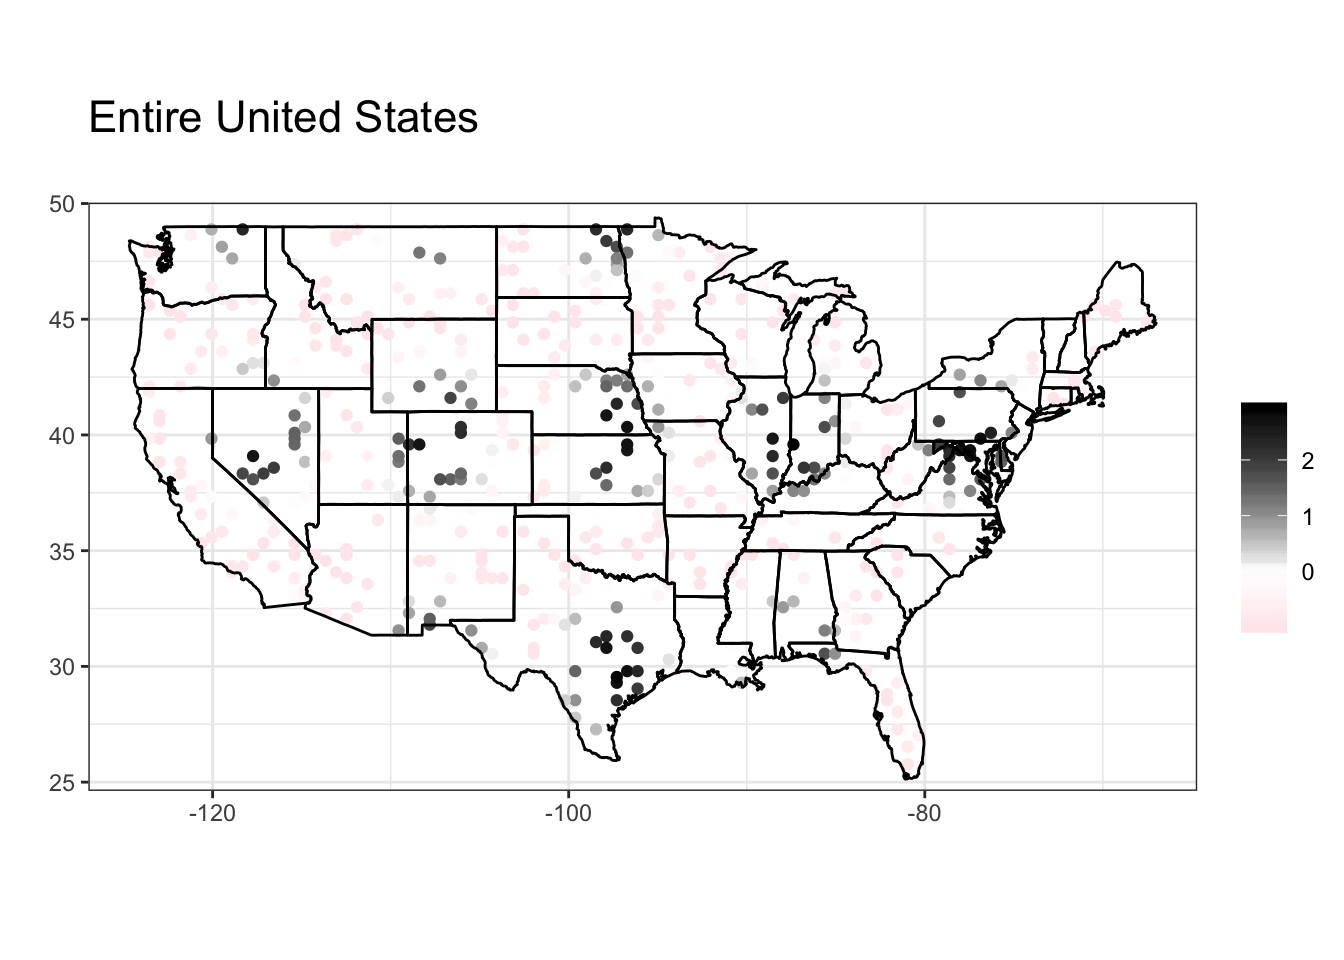
\includegraphics{STAT-5413_files/figure-latex/unnamed-chunk-32-3.pdf}

\begin{Shaded}
\begin{Highlighting}[]
\CommentTok{## Truncate the southeastern US}
\NormalTok{dat }\OperatorTok
\StringTok{    }\KeywordTok{subset}\NormalTok{(inUS) }\OperatorTok
\StringTok{    }\CommentTok{## sample 500 points at random}
\StringTok{    }\KeywordTok{sample_n}\NormalTok{(}\DecValTok{500}\NormalTok{) }\OperatorTok
\StringTok{    }\KeywordTok{map_points}\NormalTok{(}
        \DataTypeTok{color_low   =} \StringTok{"pink"}\NormalTok{, }
        \DataTypeTok{color_high  =} \StringTok{"black"}\NormalTok{,}
        \DataTypeTok{zeroiswhite =} \OtherTok{TRUE}\NormalTok{, }
        \DataTypeTok{xlim        =} \KeywordTok{c}\NormalTok{(}\OperatorTok{-}\DecValTok{95}\NormalTok{, }\DecValTok{-75}\NormalTok{),}
        \DataTypeTok{ylim        =} \KeywordTok{c}\NormalTok{(}\DecValTok{25}\NormalTok{, }\FloatTok{37.5}\NormalTok{),}
        \DataTypeTok{mainTitle   =} \StringTok{"Southeastern United States"}\NormalTok{,}
        \DataTypeTok{legendTitle =} \StringTok{"Widgets"}
\NormalTok{    )}
\end{Highlighting}
\end{Shaded}

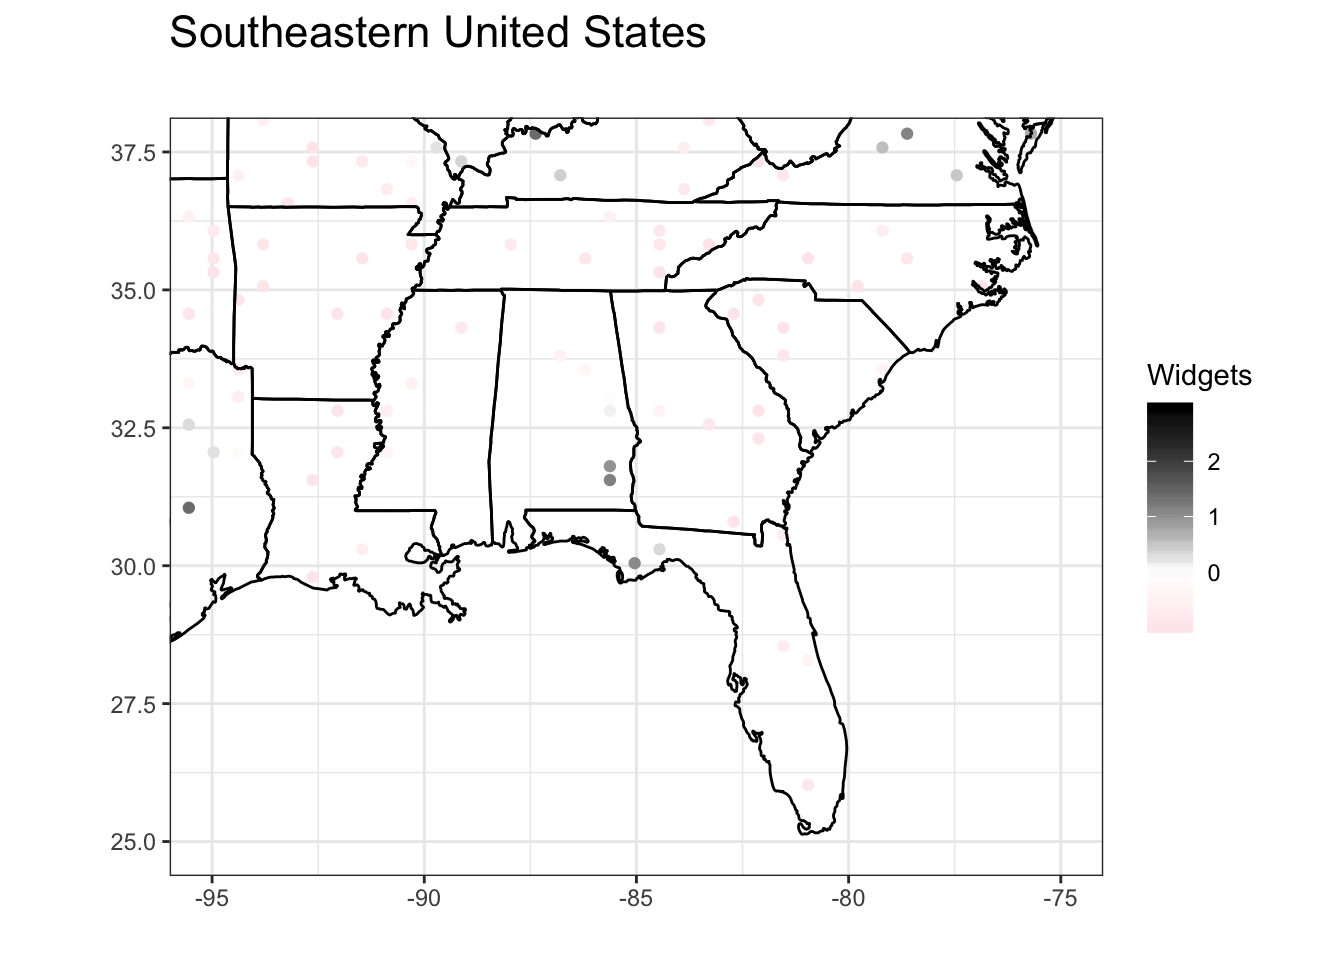
\includegraphics{STAT-5413_files/figure-latex/unnamed-chunk-32-4.pdf}

Heatmaps can also be used for plotting. In general, there are two ggplot geoms that are useful for spatial data: \emph{geom\_tile} is good for irregularly spaced data, \emph{geom\_raster} is best for regularly spaced data as it is faster to process.

\begin{Shaded}
\begin{Highlighting}[]
\CommentTok{## Function to generate maps}
\NormalTok{map_heat <-}\StringTok{ }\ControlFlowTok{function}\NormalTok{ (dat,}
                      \DataTypeTok{color_low =} \StringTok{"white"}\NormalTok{, }\DataTypeTok{color_high =} \StringTok{"darkred"}\NormalTok{, }
                      \DataTypeTok{color_na =} \KeywordTok{gray}\NormalTok{(}\FloatTok{0.9}\NormalTok{), }\DataTypeTok{zeroiswhite =} \OtherTok{FALSE}\NormalTok{,}
                      \DataTypeTok{xlim =} \OtherTok{NULL}\NormalTok{, }\DataTypeTok{ylim =} \OtherTok{NULL}\NormalTok{, }\DataTypeTok{zlim =} \OtherTok{NULL}\NormalTok{,}
                      \DataTypeTok{mainTitle =} \OtherTok{NULL}\NormalTok{, }\DataTypeTok{legendTitle =} \StringTok{""}\NormalTok{,}
                      \DataTypeTok{geom =} \StringTok{"raster"}\NormalTok{) \{}
    \KeywordTok{library}\NormalTok{(ggplot2)}
    
    \CommentTok{## check if the data.fram dat contains the correct variables}
    \ControlFlowTok{if}\NormalTok{ (}\KeywordTok{is.null}\NormalTok{(dat}\OperatorTok{$}\NormalTok{lon)) \{ }\KeywordTok{stop}\NormalTok{(}\StringTok{'The data.frame dat must contain a "lon" variable'}\NormalTok{) \}}
    \ControlFlowTok{if}\NormalTok{ (}\KeywordTok{is.null}\NormalTok{(dat}\OperatorTok{$}\NormalTok{lat)) \{ }\KeywordTok{stop}\NormalTok{(}\StringTok{'The data.frame dat must contain a "lat" variable'}\NormalTok{) \}}
    \ControlFlowTok{if}\NormalTok{ (}\KeywordTok{is.null}\NormalTok{(dat}\OperatorTok{$}\NormalTok{y))   \{ }\KeywordTok{stop}\NormalTok{(}\StringTok{'The data.frame dat must contain a "y" variable'}\NormalTok{) \}}
    \ControlFlowTok{if}\NormalTok{ (}\OperatorTok{!}\NormalTok{(geom }\OperatorTok\StringTok{ }\KeywordTok{c}\NormalTok{(}\StringTok{"raster"}\NormalTok{, }\StringTok{"tile"}\NormalTok{))) \{ }\KeywordTok{stop}\NormalTok{(}\StringTok{'The only options for geom are "raster" or "tile"'}\NormalTok{) \} }
    
    \CommentTok{# Store the base data of the underlying map}
\NormalTok{    states <-}\StringTok{ }\KeywordTok{map_data}\NormalTok{(}\StringTok{"state"}\NormalTok{)}
    
    \CommentTok{# Set limits for x, y, z if not specified as parameters}
    \ControlFlowTok{if}\NormalTok{ (}\KeywordTok{is.null}\NormalTok{(xlim)) \{ xlim <-}\StringTok{ }\KeywordTok{range}\NormalTok{(dat}\OperatorTok{$}\NormalTok{lon, }\DataTypeTok{na.rm =} \OtherTok{TRUE}\NormalTok{) \}}
    \ControlFlowTok{if}\NormalTok{ (}\KeywordTok{is.null}\NormalTok{(ylim)) \{ ylim <-}\StringTok{ }\KeywordTok{range}\NormalTok{(dat}\OperatorTok{$}\NormalTok{lat, }\DataTypeTok{na.rm =} \OtherTok{TRUE}\NormalTok{) \}}
    \ControlFlowTok{if}\NormalTok{ (}\KeywordTok{is.null}\NormalTok{(zlim)) \{ zlim <-}\StringTok{ }\KeywordTok{range}\NormalTok{(dat}\OperatorTok{$}\NormalTok{y, }\DataTypeTok{na.rm =} \OtherTok{TRUE}\NormalTok{) \}}
    
    \CommentTok{# Create the plot}
\NormalTok{    p <-}\StringTok{ }\KeywordTok{ggplot}\NormalTok{(dat, }\KeywordTok{aes}\NormalTok{(}\DataTypeTok{x =}\NormalTok{ lon, }\DataTypeTok{y =}\NormalTok{ lat)) }\OperatorTok{+}
\StringTok{        }\KeywordTok{theme_bw}\NormalTok{()}
\NormalTok{    p <-}\StringTok{ }\NormalTok{p }\OperatorTok{+}\StringTok{ }\KeywordTok{theme}\NormalTok{(}\DataTypeTok{plot.title =} \KeywordTok{element_text}\NormalTok{(}\DataTypeTok{size =} \KeywordTok{rel}\NormalTok{(}\FloatTok{1.5}\NormalTok{)))}
    \ControlFlowTok{if}\NormalTok{ (geom }\OperatorTok{==}\StringTok{ "raster"}\NormalTok{) \{}
\NormalTok{        p <-}\StringTok{ }\NormalTok{p }\OperatorTok{+}\StringTok{ }\KeywordTok{geom_raster}\NormalTok{(}\KeywordTok{aes}\NormalTok{(}\DataTypeTok{fill =}\NormalTok{ y))}
\NormalTok{    \}}
    \ControlFlowTok{if}\NormalTok{ (geom }\OperatorTok{==}\StringTok{ "tile"}\NormalTok{) \{}
\NormalTok{        p <-}\StringTok{ }\NormalTok{p }\OperatorTok{+}\StringTok{ }\KeywordTok{geom_tile}\NormalTok{(}\KeywordTok{aes}\NormalTok{(}\DataTypeTok{fill =}\NormalTok{ y))}
\NormalTok{    \}}
    \CommentTok{## add in the map}
\NormalTok{    p <-}\StringTok{ }\NormalTok{p }\OperatorTok{+}\StringTok{ }\KeywordTok{geom_polygon}\NormalTok{(}\DataTypeTok{data =}\NormalTok{ states, }\KeywordTok{aes}\NormalTok{(}\DataTypeTok{x =}\NormalTok{ long, }\DataTypeTok{y =}\NormalTok{ lat, }\DataTypeTok{group =}\NormalTok{ group), }
                          \DataTypeTok{colour =} \StringTok{"black"}\NormalTok{, }\DataTypeTok{fill =} \OtherTok{NA}\NormalTok{) }
    \CommentTok{## a 1.3 coordinate ratio is visually appealing}
\NormalTok{    p <-}\StringTok{ }\NormalTok{p }\OperatorTok{+}\StringTok{ }\KeywordTok{coord_fixed}\NormalTok{(}\DataTypeTok{ratio =} \FloatTok{1.3}\NormalTok{, }\DataTypeTok{xlim =}\NormalTok{ xlim, }\DataTypeTok{ylim =}\NormalTok{ ylim)}
\NormalTok{    p <-}\StringTok{ }\NormalTok{p }\OperatorTok{+}\StringTok{ }\KeywordTok{labs}\NormalTok{(}\DataTypeTok{title =} \KeywordTok{paste}\NormalTok{(mainTitle, }\StringTok{"}\CharTok{\textbackslash{}n}\StringTok{"}\NormalTok{, }\DataTypeTok{sep=}\StringTok{""}\NormalTok{), }\DataTypeTok{x =} \StringTok{""}\NormalTok{, }\DataTypeTok{y =} \StringTok{""}\NormalTok{)}
    \ControlFlowTok{if}\NormalTok{(zeroiswhite)\{}
\NormalTok{        p <-}\StringTok{ }\NormalTok{p }\OperatorTok{+}\StringTok{ }\KeywordTok{scale_colour_gradient2}\NormalTok{(}
            \DataTypeTok{low      =}\NormalTok{  color_low, }
            \DataTypeTok{high     =}\NormalTok{ color_high,}
            \DataTypeTok{na.value =}\NormalTok{ color_na,}
            \DataTypeTok{limits   =}\NormalTok{ zlim,}
            \DataTypeTok{name     =}\NormalTok{ legendTitle}
\NormalTok{        ) }
\NormalTok{    \}}
    \ControlFlowTok{if}\NormalTok{(}\OperatorTok{!}\NormalTok{zeroiswhite)\{}
\NormalTok{        p <-}\StringTok{ }\NormalTok{p }\OperatorTok{+}\StringTok{ }\KeywordTok{scale_colour_gradient}\NormalTok{(}
            \DataTypeTok{low      =}\NormalTok{ color_low, }
            \DataTypeTok{high     =}\NormalTok{ color_high,}
            \DataTypeTok{na.value =}\NormalTok{ color_na,}
            \DataTypeTok{limits   =}\NormalTok{ zlim,}
            \DataTypeTok{name     =}\NormalTok{ legendTitle}
\NormalTok{        ) }
\NormalTok{    \}}
    \KeywordTok{return}\NormalTok{(p)  }
\NormalTok{\}}
\end{Highlighting}
\end{Shaded}

\begin{Shaded}
\begin{Highlighting}[]
\CommentTok{## Subset only the US}
\NormalTok{dat }\OperatorTok
\StringTok{    }\KeywordTok{subset}\NormalTok{(inUS) }\OperatorTok
\StringTok{    }\KeywordTok{map_heat}\NormalTok{(}
        \DataTypeTok{color_low  =} \StringTok{"blue"}\NormalTok{, }
        \DataTypeTok{color_high =} \StringTok{"yellow"}\NormalTok{,}
        \DataTypeTok{mainTitle  =} \StringTok{"Entire United States"}\NormalTok{,}
        \DataTypeTok{geom =} \StringTok{"raster"}
\NormalTok{    )}
\end{Highlighting}
\end{Shaded}

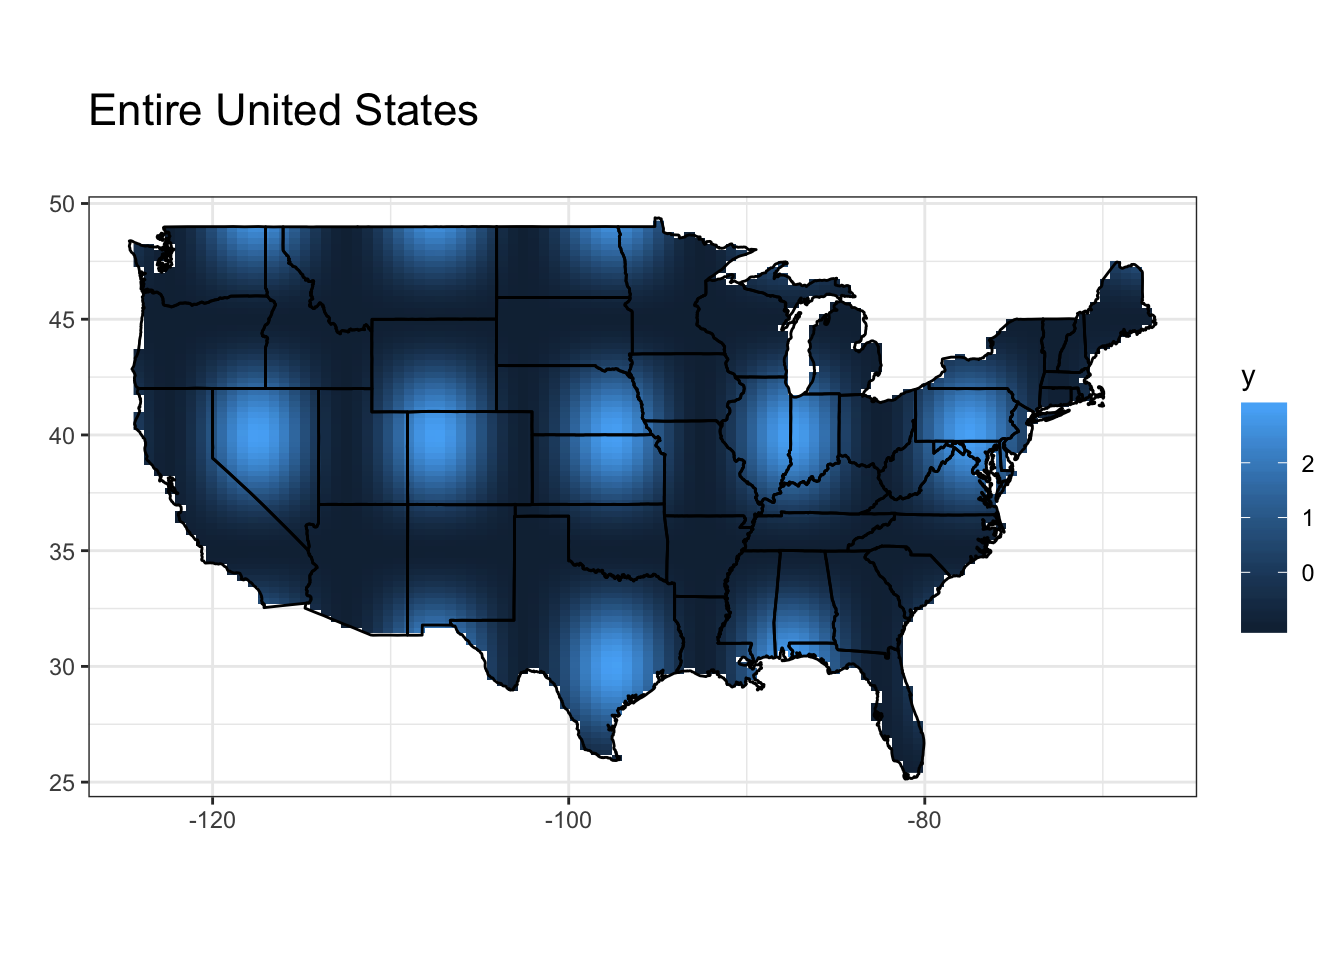
\includegraphics{STAT-5413_files/figure-latex/unnamed-chunk-34-1.pdf}

\begin{Shaded}
\begin{Highlighting}[]
\CommentTok{## Subset only the US}
\NormalTok{dat }\OperatorTok
\StringTok{    }\KeywordTok{subset}\NormalTok{(inUS) }\OperatorTok
\StringTok{    }\KeywordTok{map_heat}\NormalTok{(}
        \DataTypeTok{color_low  =} \StringTok{"blue"}\NormalTok{, }
        \DataTypeTok{color_high =} \StringTok{"yellow"}\NormalTok{,}
        \DataTypeTok{mainTitle  =} \StringTok{"Entire United States"}\NormalTok{,}
        \DataTypeTok{geom =} \StringTok{"tile"}
\NormalTok{    )}
\end{Highlighting}
\end{Shaded}

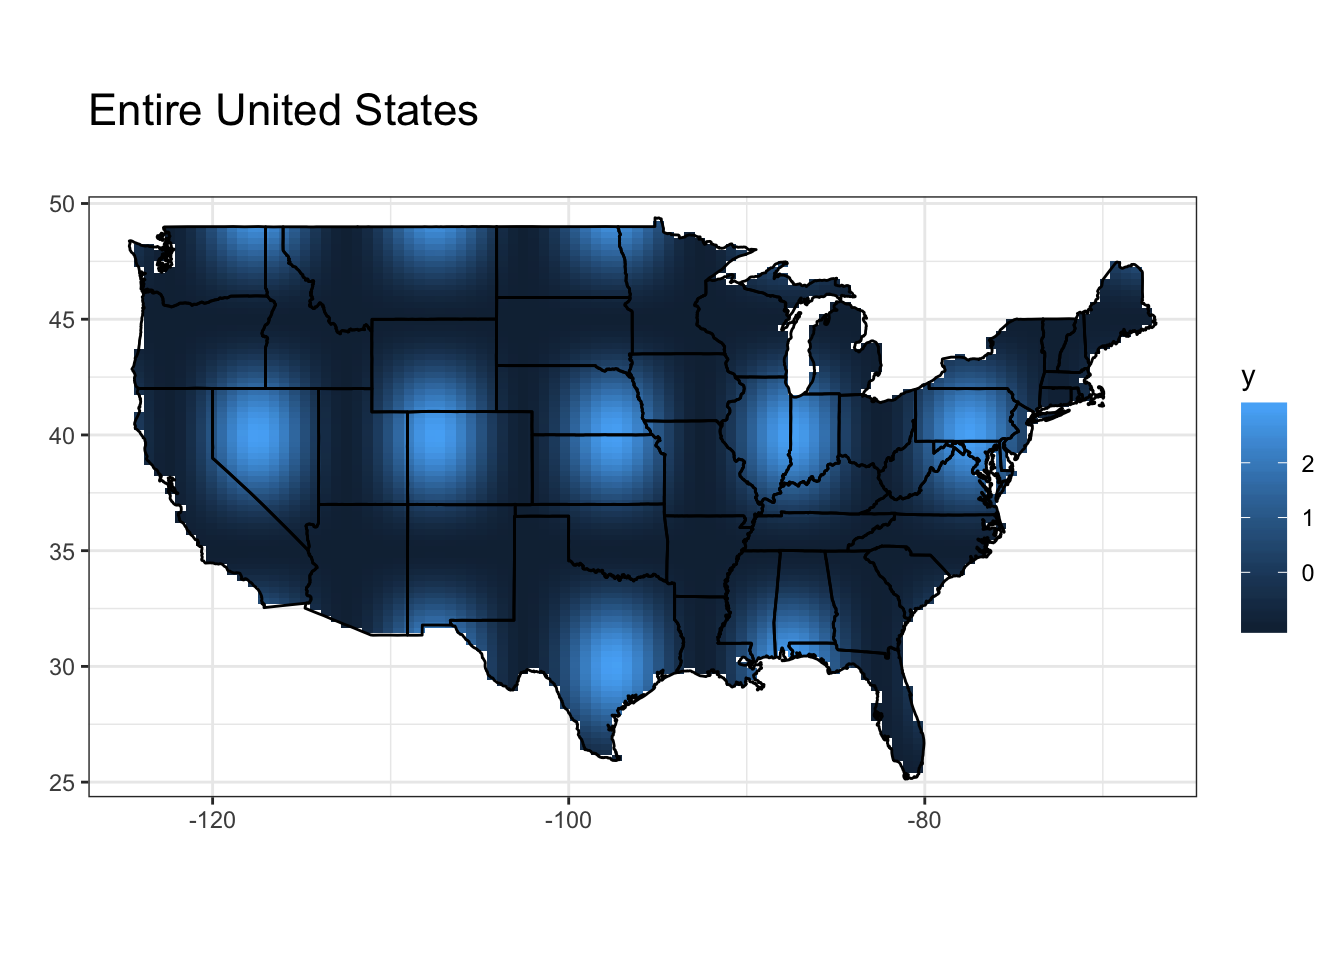
\includegraphics{STAT-5413_files/figure-latex/unnamed-chunk-34-2.pdf}

\begin{Shaded}
\begin{Highlighting}[]
\CommentTok{## Subsample the data}
\NormalTok{dat }\OperatorTok
\StringTok{    }\KeywordTok{subset}\NormalTok{(inUS) }\OperatorTok
\StringTok{    }\KeywordTok{sample_n}\NormalTok{(}\DecValTok{1000}\NormalTok{) }\OperatorTok
\StringTok{    }\KeywordTok{map_heat}\NormalTok{(}
        \DataTypeTok{color_low  =} \StringTok{"blue"}\NormalTok{, }
        \DataTypeTok{color_high =} \StringTok{"green"}\NormalTok{,}
        \DataTypeTok{mainTitle  =} \StringTok{"Entire United States"}\NormalTok{,}
        \DataTypeTok{geom =} \StringTok{"raster"}
\NormalTok{    )}
\end{Highlighting}
\end{Shaded}

\begin{verbatim}
## Warning in f(...): Raster pixels are placed at uneven horizontal intervals and
## will be shifted. Consider using geom_tile() instead.
\end{verbatim}

\begin{verbatim}
## Warning in f(...): Raster pixels are placed at uneven vertical intervals and
## will be shifted. Consider using geom_tile() instead.
\end{verbatim}

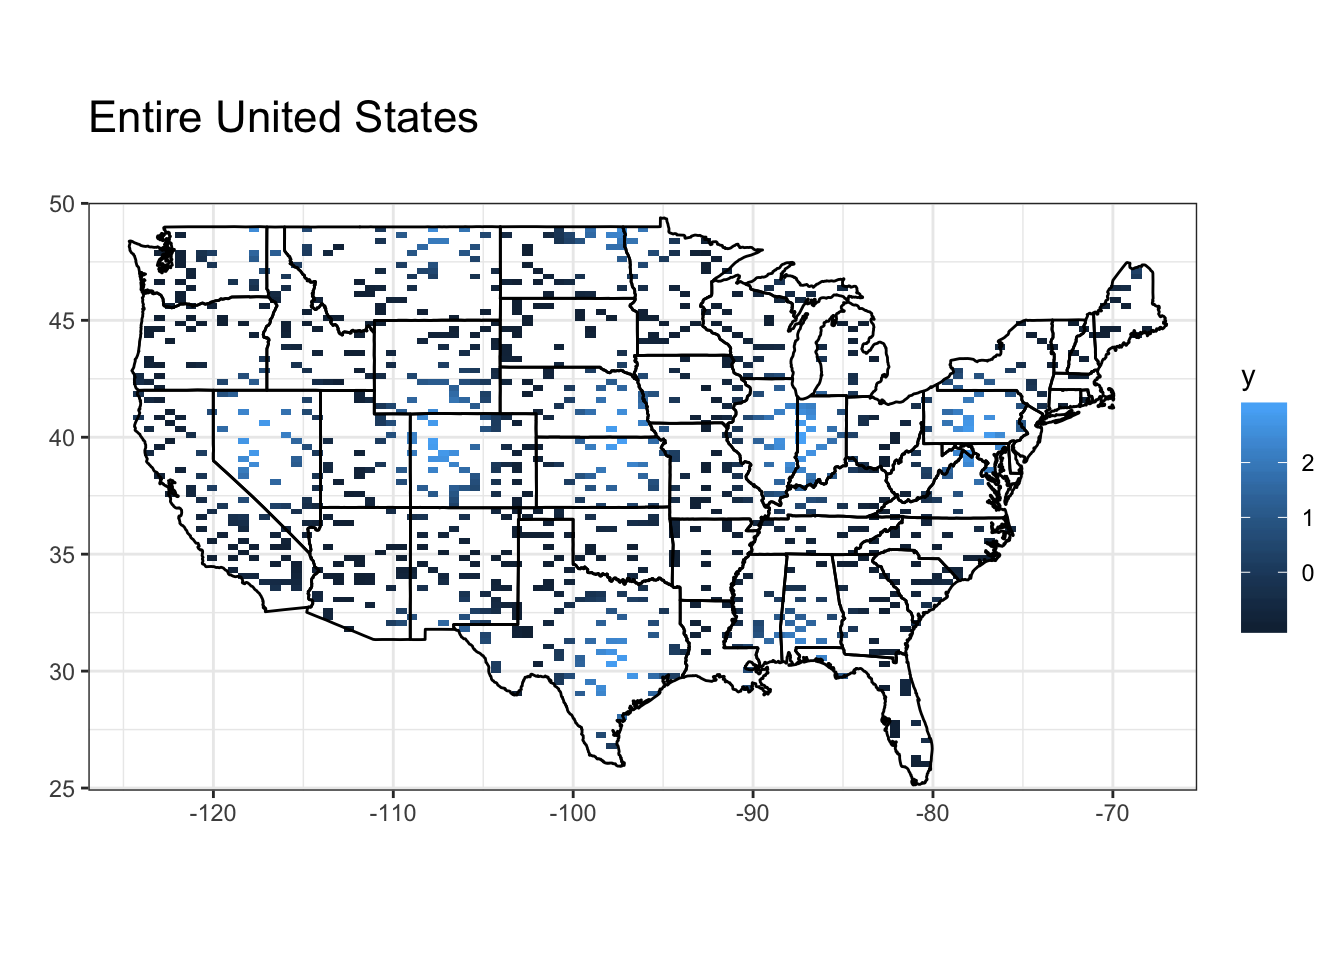
\includegraphics{STAT-5413_files/figure-latex/unnamed-chunk-35-1.pdf}

\begin{Shaded}
\begin{Highlighting}[]
\CommentTok{## Subsample the data}
\NormalTok{dat }\OperatorTok
\StringTok{    }\KeywordTok{subset}\NormalTok{(inUS) }\OperatorTok
\StringTok{    }\KeywordTok{sample_n}\NormalTok{(}\DecValTok{1000}\NormalTok{) }\OperatorTok
\StringTok{    }\KeywordTok{map_heat}\NormalTok{(}
        \DataTypeTok{color_low  =} \StringTok{"pink"}\NormalTok{, }
        \DataTypeTok{color_high =} \StringTok{"black"}\NormalTok{,}
        \DataTypeTok{mainTitle  =} \StringTok{"Entire United States"}\NormalTok{,}
        \DataTypeTok{geom =} \StringTok{"tile"}
\NormalTok{    )}
\end{Highlighting}
\end{Shaded}

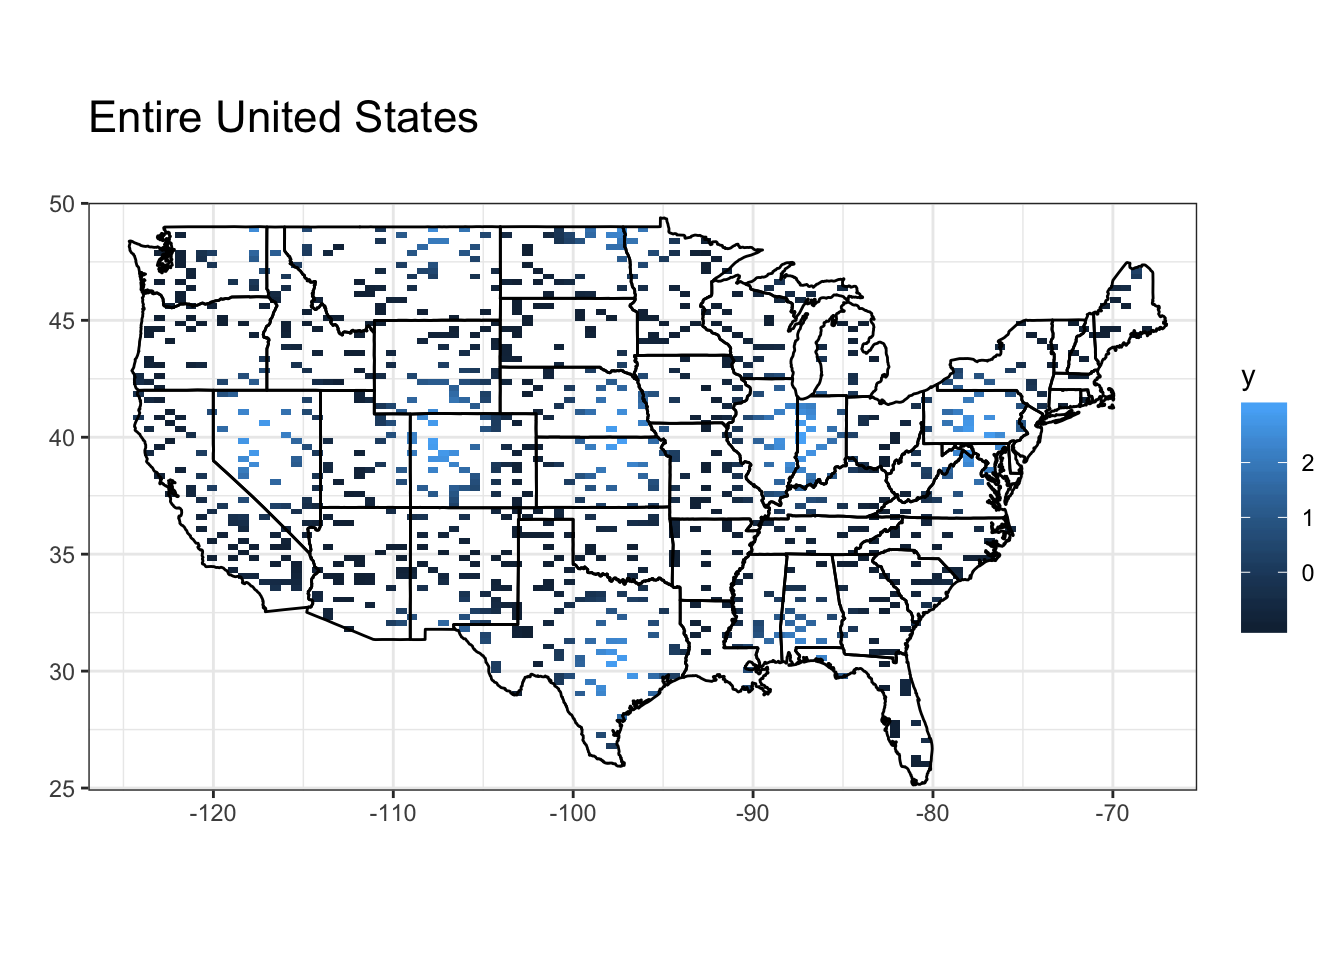
\includegraphics{STAT-5413_files/figure-latex/unnamed-chunk-36-1.pdf}

\begin{itemize}
\tightlist
\item
  Plotting spatial data using google maps
\end{itemize}

\begin{Shaded}
\begin{Highlighting}[]
\CommentTok{## longitude and latitude of approximately the center of Arkansas}
\NormalTok{arkansas_center <-}\StringTok{ }\KeywordTok{c}\NormalTok{(}\OperatorTok{-}\FloatTok{92.33}\NormalTok{, }\FloatTok{35.00}\NormalTok{) }

\KeywordTok{library}\NormalTok{(maps)}
\KeywordTok{library}\NormalTok{(ggplot2)}
\KeywordTok{library}\NormalTok{(ggmap)}
\end{Highlighting}
\end{Shaded}

\begin{verbatim}
## Google's Terms of Service: https://cloud.google.com/maps-platform/terms/.
\end{verbatim}

\begin{verbatim}
## Please cite ggmap if you use it! See citation("ggmap") for details.
\end{verbatim}

\begin{Shaded}
\begin{Highlighting}[]
\NormalTok{lon <-}\StringTok{ }\NormalTok{arkansas_center[}\DecValTok{1}\NormalTok{] }\OperatorTok{+}\StringTok{ }\KeywordTok{seq}\NormalTok{(}\OperatorTok{-}\DecValTok{2}\NormalTok{, }\DecValTok{2}\NormalTok{, }\DataTypeTok{length =} \DecValTok{10}\NormalTok{)   }
\NormalTok{lat <-}\StringTok{ }\NormalTok{arkansas_center[}\DecValTok{2}\NormalTok{] }\OperatorTok{+}\StringTok{ }\KeywordTok{seq}\NormalTok{(}\OperatorTok{-}\DecValTok{2}\NormalTok{, }\DecValTok{2}\NormalTok{, }\DataTypeTok{length =} \DecValTok{10}\NormalTok{)   }
\NormalTok{s   <-}\StringTok{ }\KeywordTok{expand.grid}\NormalTok{(lon, lat)}

\KeywordTok{head}\NormalTok{(lon)}
\end{Highlighting}
\end{Shaded}

\begin{verbatim}
## [1] -94.33000 -93.88556 -93.44111 -92.99667 -92.55222 -92.10778
\end{verbatim}

\begin{Shaded}
\begin{Highlighting}[]
\KeywordTok{head}\NormalTok{(lat) }
\end{Highlighting}
\end{Shaded}

\begin{verbatim}
## [1] 33.00000 33.44444 33.88889 34.33333 34.77778 35.22222
\end{verbatim}

\begin{Shaded}
\begin{Highlighting}[]
\KeywordTok{str}\NormalTok{(s)}
\end{Highlighting}
\end{Shaded}

\begin{verbatim}
## 'data.frame':    100 obs. of  2 variables:
##  $ Var1: num  -94.3 -93.9 -93.4 -93 -92.6 ...
##  $ Var2: num  33 33 33 33 33 33 33 33 33 33 ...
##  - attr(*, "out.attrs")=List of 2
##   ..$ dim     : int  10 10
##   ..$ dimnames:List of 2
##   .. ..$ Var1: chr  "Var1=-94.33000" "Var1=-93.88556" "Var1=-93.44111" "Var1=-92.99667" ...
##   .. ..$ Var2: chr  "Var2=33.00000" "Var2=33.44444" "Var2=33.88889" "Var2=34.33333" ...
\end{verbatim}

\begin{Shaded}
\begin{Highlighting}[]
\KeywordTok{plot}\NormalTok{(s)}
\KeywordTok{points}\NormalTok{(arkansas_center, }\DataTypeTok{pch =} \DecValTok{19}\NormalTok{, }\DataTypeTok{col =} \DecValTok{2}\NormalTok{)}
\end{Highlighting}
\end{Shaded}

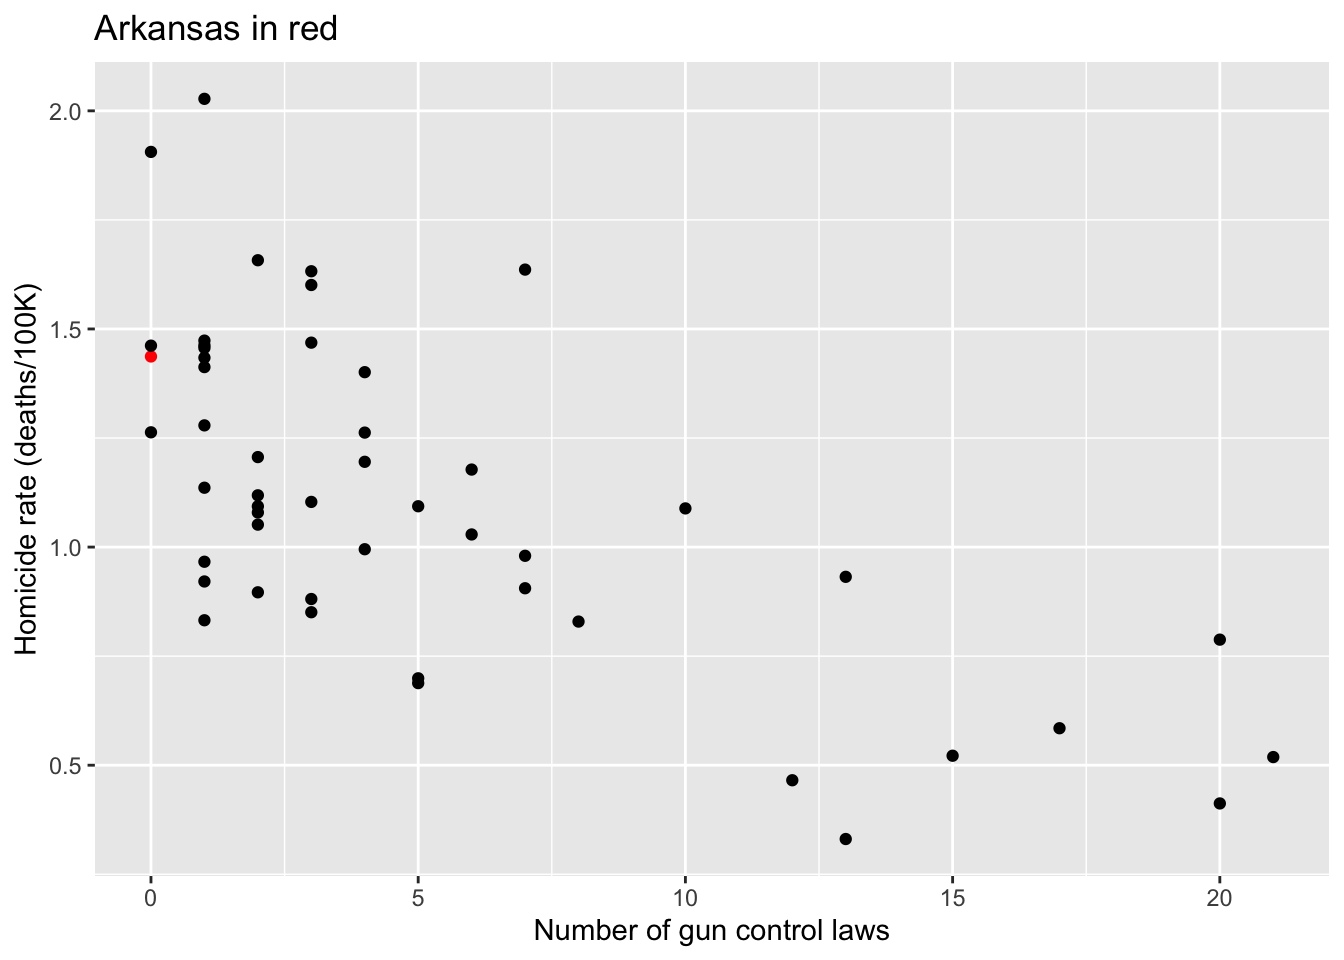
\includegraphics{STAT-5413_files/figure-latex/unnamed-chunk-37-1.pdf}

\begin{Shaded}
\begin{Highlighting}[]
\NormalTok{dat <-}\StringTok{ }\KeywordTok{data.frame}\NormalTok{(}\DataTypeTok{lon =}\NormalTok{ lon, }\DataTypeTok{lat =}\NormalTok{ lat)}
\end{Highlighting}
\end{Shaded}

Using Google maps requires registration of a key. See \url{https://www.littlemissdata.com/blog/maps} for details.

\begin{itemize}
\tightlist
\item
  Plotting areal data
  The example is from \url{https://www4.stat.ncsu.edu/~reich/SpatialStats/code/Guns.pdf} taken from \url{https://www.thelancet.com/journals/lancet/article/PIIS0140-6736(15)01026-0/fulltext}
\end{itemize}

\begin{Shaded}
\begin{Highlighting}[]
\CommentTok{## process the guns data}
\CommentTok{# load(here::here("data", "guns.RData"))}
\CommentTok{# names(Y)[1:5]}
\CommentTok{# region  <- tolower(names(Y))}
\CommentTok{# region[1:5]}
\CommentTok{# rate    <- 10000*Y/N}
\CommentTok{# numlaws <- rowSums(X)}
\CommentTok{# crime   <- data.frame(Y=Y,N=N,rate=rate,X=X,numlaws,region=region)}
\CommentTok{# dat <- data.frame(}
\CommentTok{#     deaths_2010             = Y,}
\CommentTok{#     population              = N,}
\CommentTok{#     deaths_per_10000        = Z[, 1],}
\CommentTok{#     firearm_quartile        = Z[, 2],}
\CommentTok{#     unemployment_quartile   = Z[, 3],}
\CommentTok{#     non_firearm_homocide    = Z[, 4],}
\CommentTok{#     firearm_export_quartile = Z[, 5],}
\CommentTok{#     numlaws                 = apply(X, 1, sum),}
\CommentTok{#     region                  = region}
\CommentTok{# )}
\CommentTok{# save(dat, file = here::here("data", "guns_processed.RData"))}
\KeywordTok{load}\NormalTok{(here}\OperatorTok{::}\KeywordTok{here}\NormalTok{(}\StringTok{"data"}\NormalTok{, }\StringTok{"guns_processed.RData"}\NormalTok{))}

\CommentTok{## mutate a death rate}
\NormalTok{dat <-}\StringTok{ }\NormalTok{dat }\OperatorTok
\StringTok{    }\KeywordTok{mutate}\NormalTok{(}\DataTypeTok{rate =} \DecValTok{10000} \OperatorTok{*}\StringTok{ }\NormalTok{deaths_}\DecValTok{2010} \OperatorTok{/}\StringTok{ }\NormalTok{population)}

\NormalTok{dat }\OperatorTok
\StringTok{    }\KeywordTok{ggplot}\NormalTok{(}\KeywordTok{aes}\NormalTok{(}\DataTypeTok{x =}\NormalTok{ numlaws, }\DataTypeTok{y =}\NormalTok{ rate, }\DataTypeTok{color =}\NormalTok{ region }\OperatorTok{==}\StringTok{ "arkansas"}\NormalTok{)) }\OperatorTok{+}
\StringTok{    }\KeywordTok{geom_point}\NormalTok{() }\OperatorTok{+}
\StringTok{    }\KeywordTok{scale_color_manual}\NormalTok{(}\DataTypeTok{values =} \KeywordTok{c}\NormalTok{(}\StringTok{"black"}\NormalTok{, }\StringTok{"red"}\NormalTok{)) }\OperatorTok{+}
\StringTok{    }\KeywordTok{xlab}\NormalTok{(}\StringTok{"Number of gun control laws"}\NormalTok{) }\OperatorTok{+}
\StringTok{    }\KeywordTok{ylab}\NormalTok{(}\StringTok{"Homicide rate (deaths/100K)"}\NormalTok{) }\OperatorTok{+}
\StringTok{    }\KeywordTok{ggtitle}\NormalTok{(}\StringTok{"Arkansas in red"}\NormalTok{) }\OperatorTok{+}
\StringTok{    }\KeywordTok{theme}\NormalTok{(}\DataTypeTok{legend.position =} \StringTok{"none"}\NormalTok{)}
\end{Highlighting}
\end{Shaded}

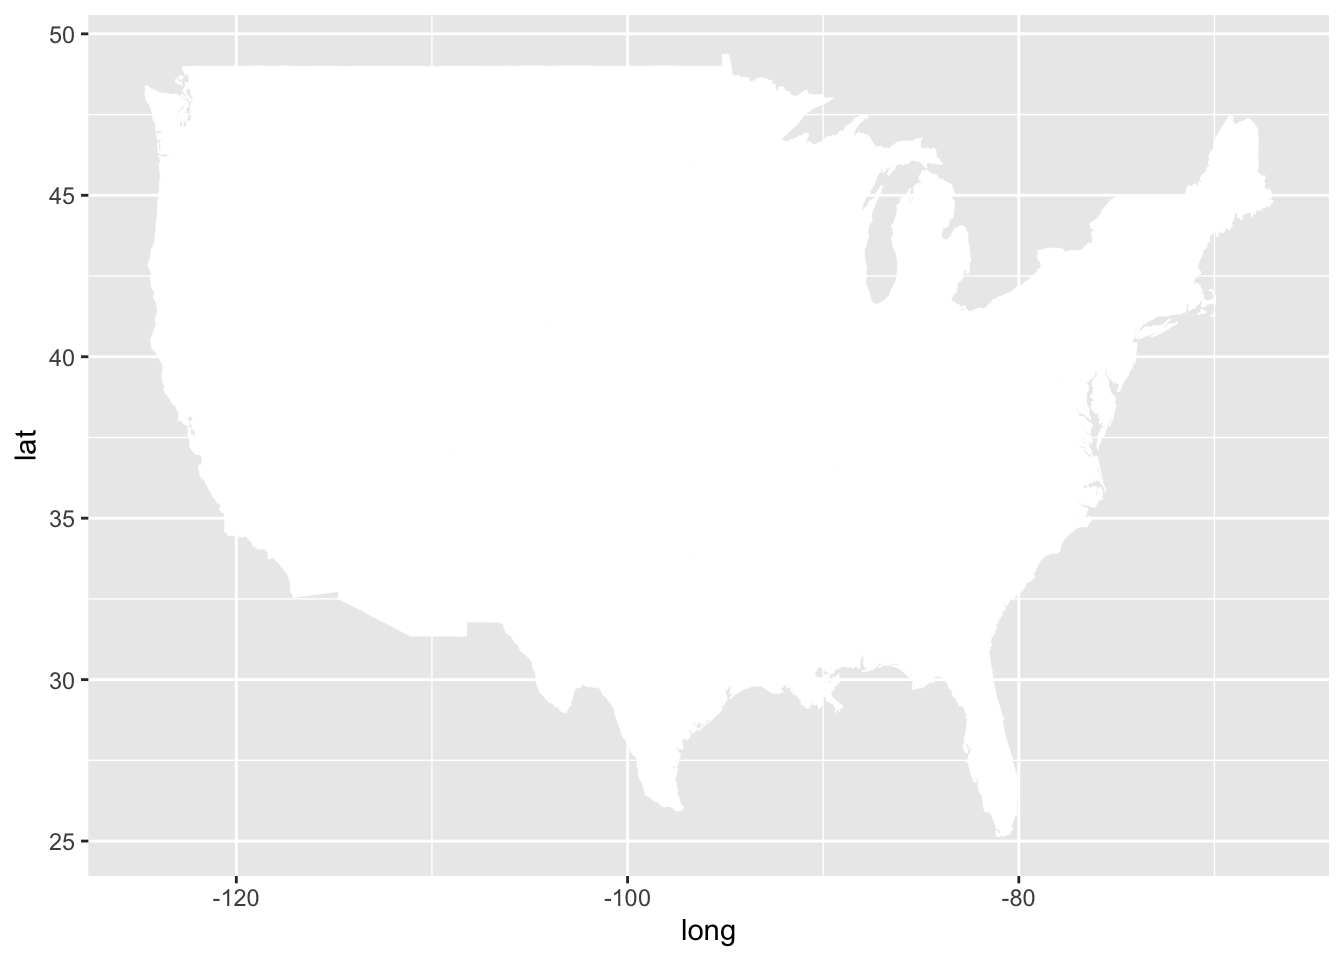
\includegraphics{STAT-5413_files/figure-latex/unnamed-chunk-38-1.pdf}

\begin{Shaded}
\begin{Highlighting}[]
\KeywordTok{lm}\NormalTok{(rate }\OperatorTok{~}\StringTok{ }\NormalTok{numlaws, }\DataTypeTok{data =}\NormalTok{ dat) }\OperatorTok\StringTok{ }\KeywordTok{summary}\NormalTok{()}
\end{Highlighting}
\end{Shaded}

\begin{verbatim}
## 
## Call:
## lm(formula = rate ~ numlaws, data = dat)
## 
## Residuals:
##      Min       1Q   Median       3Q      Max 
## -0.46715 -0.16720 -0.02576  0.16171  0.72809 
## 
## Coefficients:
##              Estimate Std. Error t value Pr(>|t|)    
## (Intercept)  1.344693   0.055145  24.385  < 2e-16 ***
## numlaws     -0.045276   0.007302  -6.201 1.24e-07 ***
## ---
## Signif. codes:  0 '***' 0.001 '**' 0.01 '*' 0.05 '.' 0.1 ' ' 1
## 
## Residual standard error: 0.2867 on 48 degrees of freedom
## Multiple R-squared:  0.4448, Adjusted R-squared:  0.4332 
## F-statistic: 38.45 on 1 and 48 DF,  p-value: 1.236e-07
\end{verbatim}

\begin{Shaded}
\begin{Highlighting}[]
\NormalTok{us <-}\StringTok{ }\KeywordTok{map_data}\NormalTok{(}\StringTok{"state"}\NormalTok{)}
\KeywordTok{head}\NormalTok{(us)}
\end{Highlighting}
\end{Shaded}

\begin{verbatim}
##        long      lat group order  region subregion
## 1 -87.46201 30.38968     1     1 alabama      <NA>
## 2 -87.48493 30.37249     1     2 alabama      <NA>
## 3 -87.52503 30.37249     1     3 alabama      <NA>
## 4 -87.53076 30.33239     1     4 alabama      <NA>
## 5 -87.57087 30.32665     1     5 alabama      <NA>
## 6 -87.58806 30.32665     1     6 alabama      <NA>
\end{verbatim}

\begin{Shaded}
\begin{Highlighting}[]
\NormalTok{gg <-}\StringTok{ }\KeywordTok{ggplot}\NormalTok{()}
\NormalTok{gg <-}\StringTok{ }\NormalTok{gg }\OperatorTok{+}\StringTok{ }\KeywordTok{geom_map}\NormalTok{(}\DataTypeTok{data =}\NormalTok{ us, }\DataTypeTok{map =}\NormalTok{ us,}
                    \KeywordTok{aes}\NormalTok{(}\DataTypeTok{x =}\NormalTok{ long, }\DataTypeTok{y =}\NormalTok{ lat, }\DataTypeTok{map_id =}\NormalTok{ region),}
                    \DataTypeTok{fill =} \StringTok{"#ffffff"}\NormalTok{, }\DataTypeTok{color =} \StringTok{"#ffffff"}\NormalTok{, }\DataTypeTok{size =} \FloatTok{0.15}\NormalTok{)}
\end{Highlighting}
\end{Shaded}

\begin{verbatim}
## Warning: Ignoring unknown aesthetics: x, y
\end{verbatim}

\begin{Shaded}
\begin{Highlighting}[]
\NormalTok{gg}
\end{Highlighting}
\end{Shaded}

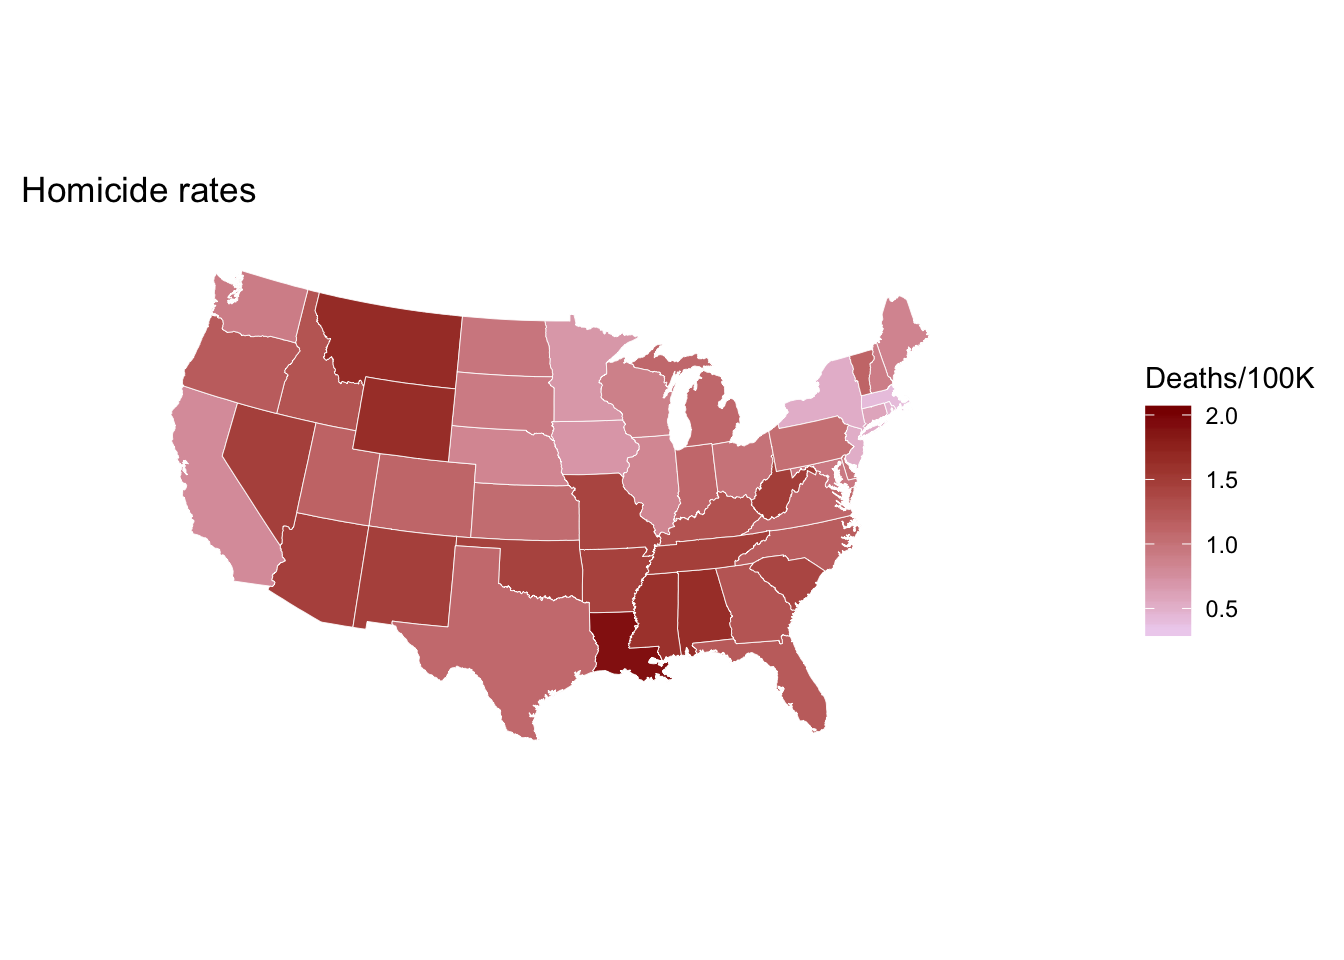
\includegraphics{STAT-5413_files/figure-latex/unnamed-chunk-39-1.pdf}

\begin{Shaded}
\begin{Highlighting}[]
\NormalTok{gg <-}\StringTok{ }\NormalTok{gg }\OperatorTok{+}\StringTok{ }\KeywordTok{geom_map}\NormalTok{(}
    \DataTypeTok{data =}\NormalTok{ dat, }
    \DataTypeTok{map =}\NormalTok{ us,}
    \KeywordTok{aes}\NormalTok{(}\DataTypeTok{fill =}\NormalTok{ rate, }\DataTypeTok{map_id =}\NormalTok{ region),}
    \DataTypeTok{color =} \StringTok{"#ffffff"}\NormalTok{, }\DataTypeTok{size =} \FloatTok{0.15}
\NormalTok{)}

\NormalTok{gg <-}\StringTok{ }\NormalTok{gg }\OperatorTok{+}\StringTok{ }\KeywordTok{scale_fill_continuous}\NormalTok{(}
    \DataTypeTok{low  =} \StringTok{'thistle2'}\NormalTok{, }
    \DataTypeTok{high =} \StringTok{'darkred'}\NormalTok{, }
    \DataTypeTok{guide=} \StringTok{'colorbar'}\NormalTok{,}
    \DataTypeTok{name =} \StringTok{"Deaths/100K"}
\NormalTok{)}
\NormalTok{gg <-}\StringTok{ }\NormalTok{gg }\OperatorTok{+}\StringTok{ }\KeywordTok{labs}\NormalTok{(}\DataTypeTok{x =} \OtherTok{NULL}\NormalTok{, }\DataTypeTok{y =} \OtherTok{NULL}\NormalTok{, }\DataTypeTok{title =} \StringTok{"Homicide rates"}\NormalTok{)}
\NormalTok{gg <-}\StringTok{ }\NormalTok{gg }\OperatorTok{+}\StringTok{ }\KeywordTok{coord_map}\NormalTok{(}\StringTok{"albers"}\NormalTok{, }\DataTypeTok{lat0 =} \DecValTok{39}\NormalTok{, }\DataTypeTok{lat1 =} \DecValTok{45}\NormalTok{) }
\NormalTok{gg <-}\StringTok{ }\NormalTok{gg }\OperatorTok{+}\StringTok{ }\KeywordTok{theme}\NormalTok{(}\DataTypeTok{panel.border =} \KeywordTok{element_blank}\NormalTok{())}
\NormalTok{gg <-}\StringTok{ }\NormalTok{gg }\OperatorTok{+}\StringTok{ }\KeywordTok{theme}\NormalTok{(}\DataTypeTok{panel.background =} \KeywordTok{element_blank}\NormalTok{())}
\NormalTok{gg <-}\StringTok{ }\NormalTok{gg }\OperatorTok{+}\StringTok{ }\KeywordTok{theme}\NormalTok{(}\DataTypeTok{axis.ticks =} \KeywordTok{element_blank}\NormalTok{())}
\NormalTok{gg <-}\StringTok{ }\NormalTok{gg }\OperatorTok{+}\StringTok{ }\KeywordTok{theme}\NormalTok{(}\DataTypeTok{axis.text =} \KeywordTok{element_blank}\NormalTok{())}
\NormalTok{gg}
\end{Highlighting}
\end{Shaded}

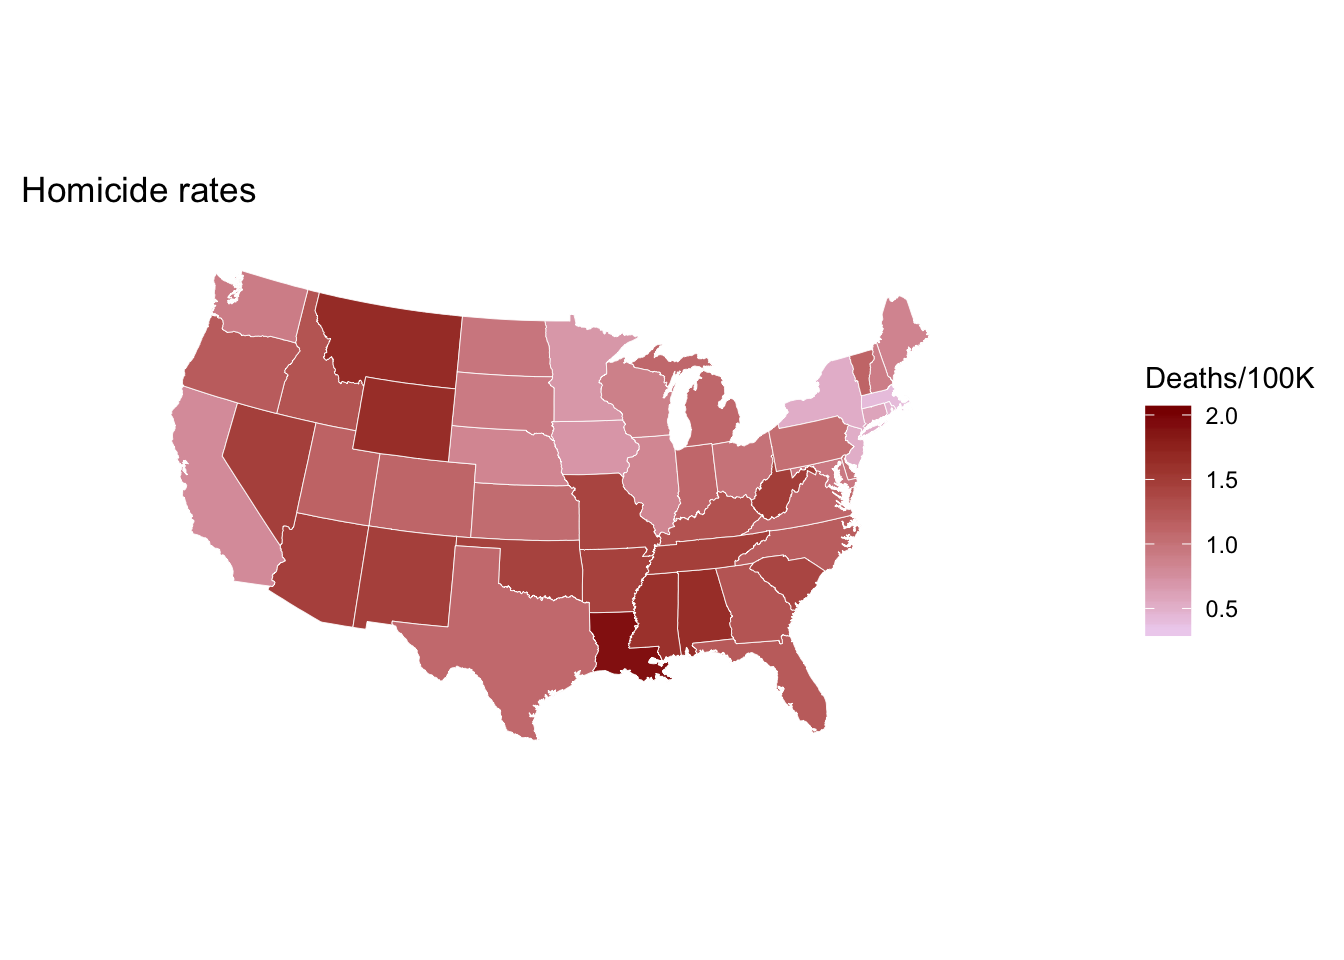
\includegraphics{STAT-5413_files/figure-latex/unnamed-chunk-40-1.pdf}

The map looks right according to

\url{http://www.deathpenaltyinfo.org/murder-rates-nationally-and-state\#MRord}

\hypertarget{in-class-activity}{%
\subsection{In Class Activity:}\label{in-class-activity}}

From \href{https://spacetimewithr.org/code}{Lab 2.1} on the textbook site

\begin{Shaded}
\begin{Highlighting}[]
\CommentTok{## Wikle, C. K., Zammit-Mangion, A., and Cressie, N. (2019), }
\CommentTok{## Spatio-Temporal Statistics with R, Boca Raton, FL: Chapman & Hall/CRC}
\CommentTok{## Copyright (c) 2019 Wikle, Zammit-Mangion, Cressie}
\CommentTok{##}
\CommentTok{## This program is free software; you can redistribute it and/or}
\CommentTok{## modify it under the terms of the GNU General Public License}
\CommentTok{## as published by the Free Software Foundation; either version 2}
\CommentTok{## of the License, or (at your option) any later version.}
\CommentTok{##}
\CommentTok{## This program is distributed in the hope that it will be useful,}
\CommentTok{## but WITHOUT ANY WARRANTY; without even the implied warranty of}
\CommentTok{## MERCHANTABILITY or FITNESS FOR A PARTICULAR PURPOSE.  See the}
\CommentTok{## GNU General Public License for more details.}

\KeywordTok{library}\NormalTok{(}\StringTok{"dplyr"}\NormalTok{)}
\KeywordTok{library}\NormalTok{(}\StringTok{"tidyr"}\NormalTok{)}
\KeywordTok{library}\NormalTok{(}\StringTok{"STRbook"}\NormalTok{)}

\CommentTok{## ------------------------------------------------------------------------}
\NormalTok{locs <-}\StringTok{ }\KeywordTok{read.table}\NormalTok{(}\KeywordTok{system.file}\NormalTok{(}\StringTok{"extdata"}\NormalTok{, }\StringTok{"Stationinfo.dat"}\NormalTok{,}
                               \DataTypeTok{package =} \StringTok{"STRbook"}\NormalTok{),}
                   \DataTypeTok{col.names =} \KeywordTok{c}\NormalTok{(}\StringTok{"id"}\NormalTok{, }\StringTok{"lat"}\NormalTok{, }\StringTok{"lon"}\NormalTok{))}
\NormalTok{Times <-}\StringTok{ }\KeywordTok{read.table}\NormalTok{(}\KeywordTok{system.file}\NormalTok{(}\StringTok{"extdata"}\NormalTok{, }\StringTok{"Times_1990.dat"}\NormalTok{,}
                                \DataTypeTok{package =} \StringTok{"STRbook"}\NormalTok{),}
                    \DataTypeTok{col.names =} \KeywordTok{c}\NormalTok{(}\StringTok{"julian"}\NormalTok{, }\StringTok{"year"}\NormalTok{, }\StringTok{"month"}\NormalTok{, }\StringTok{"day"}\NormalTok{))}
\NormalTok{Tmax <-}\StringTok{ }\KeywordTok{read.table}\NormalTok{(}\KeywordTok{system.file}\NormalTok{(}\StringTok{"extdata"}\NormalTok{, }\StringTok{"Tmax_1990.dat"}\NormalTok{,}
                               \DataTypeTok{package =} \StringTok{"STRbook"}\NormalTok{))}

\CommentTok{## ------------------------------------------------------------------------}
\KeywordTok{names}\NormalTok{(Tmax) <-}\StringTok{ }\NormalTok{locs}\OperatorTok{$}\NormalTok{id}

\CommentTok{## ------------------------------------------------------------------------}
\NormalTok{Tmax <-}\StringTok{ }\KeywordTok{cbind}\NormalTok{(Times, Tmax)}
\KeywordTok{head}\NormalTok{(}\KeywordTok{names}\NormalTok{(Tmax), }\DecValTok{10}\NormalTok{)}

\CommentTok{## ------------------------------------------------------------------------}
\NormalTok{Tmax_long <-}\StringTok{ }\KeywordTok{gather}\NormalTok{(Tmax, id, z, }\OperatorTok{-}\NormalTok{julian, }\OperatorTok{-}\NormalTok{year, }\OperatorTok{-}\NormalTok{month, }\OperatorTok{-}\NormalTok{day)}
\KeywordTok{head}\NormalTok{(Tmax_long)}

\CommentTok{## ------------------------------------------------------------------------}
\NormalTok{Tmax_long}\OperatorTok{$}\NormalTok{id <-}\StringTok{ }\KeywordTok{as.integer}\NormalTok{(Tmax_long}\OperatorTok{$}\NormalTok{id)}

\CommentTok{## -----------------------------------------------------------}
\KeywordTok{nrow}\NormalTok{(Tmax_long)}
\NormalTok{Tmax_long <-}\StringTok{ }\KeywordTok{filter}\NormalTok{(Tmax_long, }\OperatorTok{!}\NormalTok{(z }\OperatorTok{<=}\StringTok{ }\DecValTok{-9998}\NormalTok{))}
\KeywordTok{nrow}\NormalTok{(Tmax_long)}

\CommentTok{## ------------------------------------------------------------------------}
\NormalTok{Tmax_long <-}\StringTok{ }\KeywordTok{mutate}\NormalTok{(Tmax_long, }\DataTypeTok{proc =} \StringTok{"Tmax"}\NormalTok{)}
\KeywordTok{head}\NormalTok{(Tmax_long)}

\CommentTok{## ------------------------------------------------------------------------}
\KeywordTok{data}\NormalTok{(Tmin_long, }\DataTypeTok{package =} \StringTok{"STRbook"}\NormalTok{)}
\KeywordTok{data}\NormalTok{(TDP_long, }\DataTypeTok{package =} \StringTok{"STRbook"}\NormalTok{)}
\KeywordTok{data}\NormalTok{(Precip_long, }\DataTypeTok{package =} \StringTok{"STRbook"}\NormalTok{)}

\CommentTok{## ------------------------------------------------------------------------}
\NormalTok{NOAA_df_}\DecValTok{1990}\NormalTok{ <-}\StringTok{ }\KeywordTok{rbind}\NormalTok{(Tmax_long, Tmin_long, TDP_long, Precip_long)}

\CommentTok{## ------------------------------------------------------------------------}
\NormalTok{summ <-}\StringTok{ }\KeywordTok{group_by}\NormalTok{(NOAA_df_}\DecValTok{1990}\NormalTok{, year, proc) }\OperatorTok\StringTok{  }\CommentTok{# groupings}
\StringTok{    }\KeywordTok{summarise}\NormalTok{(}\DataTypeTok{mean_proc =} \KeywordTok{mean}\NormalTok{(z))          }\CommentTok{# operation}

\CommentTok{## ------------------------------------------------------------------------}
\NormalTok{NOAA_precip <-}\StringTok{ }\KeywordTok{filter}\NormalTok{(NOAA_df_}\DecValTok{1990}\NormalTok{, proc }\OperatorTok{==}\StringTok{ "Precip"} \OperatorTok{&}\StringTok{ }\NormalTok{month }\OperatorTok{==}\StringTok{ }\DecValTok{6}\NormalTok{)}
\NormalTok{summ <-}\StringTok{ }\KeywordTok{group_by}\NormalTok{(NOAA_precip, year, id) }\OperatorTok
\StringTok{    }\KeywordTok{summarise}\NormalTok{(}\DataTypeTok{days_no_precip =} \KeywordTok{sum}\NormalTok{(z }\OperatorTok{==}\StringTok{ }\DecValTok{0}\NormalTok{))}
\KeywordTok{head}\NormalTok{(summ)}

\CommentTok{## ------------------------------------------------------------------------}
\KeywordTok{median}\NormalTok{(summ}\OperatorTok{$}\NormalTok{days_no_precip)}

\CommentTok{## -------------------------------------------------------------}
\NormalTok{grps <-}\StringTok{ }\KeywordTok{group_by}\NormalTok{(NOAA_precip, year, id)}
\NormalTok{summ <-}\StringTok{ }\KeywordTok{summarise}\NormalTok{(grps, }\DataTypeTok{days_no_precip =} \KeywordTok{sum}\NormalTok{(z }\OperatorTok{==}\StringTok{ }\DecValTok{0}\NormalTok{))}

\CommentTok{## ------------------------------------------------------------------------}
\NormalTok{NOAA_df_sorted <-}\StringTok{ }\KeywordTok{arrange}\NormalTok{(NOAA_df_}\DecValTok{1990}\NormalTok{, julian, id)}

\CommentTok{## ------------------------------------------------------------------------}
\NormalTok{df1 <-}\StringTok{ }\KeywordTok{select}\NormalTok{(NOAA_df_}\DecValTok{1990}\NormalTok{, julian, z)}
\NormalTok{df2 <-}\StringTok{ }\KeywordTok{select}\NormalTok{(NOAA_df_}\DecValTok{1990}\NormalTok{, }\OperatorTok{-}\NormalTok{julian)}

\CommentTok{## ------------------------------------------------------------------------}
\NormalTok{NOAA_df_}\DecValTok{1990}\NormalTok{ <-}\StringTok{ }\KeywordTok{left_join}\NormalTok{(NOAA_df_}\DecValTok{1990}\NormalTok{, locs, }\DataTypeTok{by =} \StringTok{"id"}\NormalTok{)}

\CommentTok{## ------------------------------------------------------------------------}
\NormalTok{Tmax_long_sel <-}\StringTok{ }\KeywordTok{select}\NormalTok{(Tmax_long, julian, id, z)}
\NormalTok{Tmax_wide <-}\StringTok{ }\KeywordTok{spread}\NormalTok{(Tmax_long_sel, id, z)}
\KeywordTok{dim}\NormalTok{(Tmax_wide)}

\CommentTok{## ------------------------------------------------------------------------}
\NormalTok{M <-}\StringTok{ }\KeywordTok{select}\NormalTok{(Tmax_wide, }\OperatorTok{-}\NormalTok{julian) }\OperatorTok\StringTok{ }\KeywordTok{as.matrix}\NormalTok{()}

\CommentTok{## -----------------------------------------------------------}
\KeywordTok{library}\NormalTok{(}\StringTok{"sp"}\NormalTok{)}
\KeywordTok{library}\NormalTok{(}\StringTok{"spacetime"}\NormalTok{)}

\CommentTok{## ------------------------------------------------------------------------}
\NormalTok{NOAA_df_}\DecValTok{1990}\OperatorTok{$}\NormalTok{date <-}\StringTok{ }\KeywordTok{with}\NormalTok{(NOAA_df_}\DecValTok{1990}\NormalTok{,}
                          \KeywordTok{paste}\NormalTok{(year, month, day, }\DataTypeTok{sep =} \StringTok{"-"}\NormalTok{))}
\KeywordTok{head}\NormalTok{(NOAA_df_}\DecValTok{1990}\OperatorTok{$}\NormalTok{date, }\DecValTok{4}\NormalTok{)   }\CommentTok{# show first four elements}

\CommentTok{## ------------------------------------------------------------------------}
\NormalTok{NOAA_df_}\DecValTok{1990}\OperatorTok{$}\NormalTok{date <-}\StringTok{ }\KeywordTok{as.Date}\NormalTok{(NOAA_df_}\DecValTok{1990}\OperatorTok{$}\NormalTok{date)}
\KeywordTok{class}\NormalTok{(NOAA_df_}\DecValTok{1990}\OperatorTok{$}\NormalTok{date)}

\CommentTok{## ------------------------------------------------------------------------}
\NormalTok{Tmax_long2 <-}\StringTok{ }\KeywordTok{filter}\NormalTok{(NOAA_df_}\DecValTok{1990}\NormalTok{, proc }\OperatorTok{==}\StringTok{ "Tmax"}\NormalTok{)}
\NormalTok{STObj <-}\StringTok{ }\KeywordTok{stConstruct}\NormalTok{(}\DataTypeTok{x =}\NormalTok{ Tmax_long2,           }\CommentTok{# data set}
                     \DataTypeTok{space =} \KeywordTok{c}\NormalTok{(}\StringTok{"lon"}\NormalTok{, }\StringTok{"lat"}\NormalTok{),  }\CommentTok{# spatial fields}
                     \DataTypeTok{time =} \StringTok{"date"}\NormalTok{)            }\CommentTok{# time field}
\KeywordTok{class}\NormalTok{(STObj)}

\CommentTok{## ------------------------------------------------------------------------}
\NormalTok{spat_part <-}\StringTok{ }\KeywordTok{SpatialPoints}\NormalTok{(}\DataTypeTok{coords =}\NormalTok{ Tmax_long2[, }\KeywordTok{c}\NormalTok{(}\StringTok{"lon"}\NormalTok{, }\StringTok{"lat"}\NormalTok{)])}
\NormalTok{temp_part <-}\StringTok{ }\NormalTok{Tmax_long2}\OperatorTok{$}\NormalTok{date}
\NormalTok{STObj2 <-}\StringTok{ }\KeywordTok{STIDF}\NormalTok{(}\DataTypeTok{sp =}\NormalTok{ spat_part,}
                \DataTypeTok{time =}\NormalTok{ temp_part,}
                \DataTypeTok{data =} \KeywordTok{select}\NormalTok{(Tmax_long2, }\OperatorTok{-}\NormalTok{date, }\OperatorTok{-}\NormalTok{lon, }\OperatorTok{-}\NormalTok{lat))}
\KeywordTok{class}\NormalTok{(STObj2)}

\CommentTok{## ------------------------------------------------------------------------}
\NormalTok{spat_part <-}\StringTok{ }\KeywordTok{SpatialPoints}\NormalTok{(}\DataTypeTok{coords =}\NormalTok{ locs[, }\KeywordTok{c}\NormalTok{(}\StringTok{"lon"}\NormalTok{, }\StringTok{"lat"}\NormalTok{)])}
\NormalTok{temp_part <-}\StringTok{ }\KeywordTok{with}\NormalTok{(Times,}
                  \KeywordTok{paste}\NormalTok{(year, month, day, }\DataTypeTok{sep =} \StringTok{"-"}\NormalTok{))}
\NormalTok{temp_part <-}\StringTok{ }\KeywordTok{as.Date}\NormalTok{(temp_part)}

\CommentTok{## ------------------------------------------------------------------------}
\NormalTok{Tmax_long3 <-}\StringTok{ }\KeywordTok{gather}\NormalTok{(Tmax, id, z, }\OperatorTok{-}\NormalTok{julian, }\OperatorTok{-}\NormalTok{year, }\OperatorTok{-}\NormalTok{month, }\OperatorTok{-}\NormalTok{day)}

\CommentTok{## ------------------------------------------------------------------------}
\NormalTok{Tmax_long3}\OperatorTok{$}\NormalTok{id <-}\StringTok{ }\KeywordTok{as.integer}\NormalTok{(Tmax_long3}\OperatorTok{$}\NormalTok{id)}
\NormalTok{Tmax_long3 <-}\StringTok{ }\KeywordTok{arrange}\NormalTok{(Tmax_long3,julian,id)}

\CommentTok{## ------------------------------------------------------------------------}
\KeywordTok{all}\NormalTok{(}\KeywordTok{unique}\NormalTok{(Tmax_long3}\OperatorTok{$}\NormalTok{id) }\OperatorTok{==}\StringTok{ }\NormalTok{locs}\OperatorTok{$}\NormalTok{id)}

\CommentTok{## ------------------------------------------------------------------------}
\NormalTok{STObj3 <-}\StringTok{ }\KeywordTok{STFDF}\NormalTok{(}\DataTypeTok{sp =}\NormalTok{ spat_part,}
                \DataTypeTok{time =}\NormalTok{ temp_part,}
                \DataTypeTok{data =}\NormalTok{ Tmax_long3)}
\KeywordTok{class}\NormalTok{(STObj3)}

\CommentTok{## ------------------------------------------------------------------------}
\KeywordTok{proj4string}\NormalTok{(STObj3) <-}\StringTok{ }\KeywordTok{CRS}\NormalTok{(}\StringTok{"+proj=longlat +ellps=WGS84"}\NormalTok{)}

\CommentTok{## ------------------------------------------------------------------------}
\NormalTok{STObj3}\OperatorTok{$}\NormalTok{z[STObj3}\OperatorTok{$}\NormalTok{z }\OperatorTok{==}\StringTok{ }\DecValTok{-9999}\NormalTok{] <-}\StringTok{ }\OtherTok{NA}
\end{Highlighting}
\end{Shaded}

\hypertarget{day-4}{%
\chapter{Day 4}\label{day-4}}

\hypertarget{interactive-visualization-html-format-only}{%
\section{Interactive visualization (HTML format only)}\label{interactive-visualization-html-format-only}}

\begin{Shaded}
\begin{Highlighting}[]
\CommentTok{# install.packages("webshot")}
\CommentTok{# webshot::install_phantomjs()}
\NormalTok{DT}\OperatorTok{::}\KeywordTok{datatable}\NormalTok{(iris)}
\end{Highlighting}
\end{Shaded}

\includegraphics{STAT-5413_files/figure-latex/unnamed-chunk-42-1.pdf}

\hypertarget{day-5}{%
\chapter{Day 5}\label{day-5}}

\hypertarget{day-6}{%
\chapter{Day 6}\label{day-6}}

\hypertarget{day-5-1}{%
\chapter{Day 5}\label{day-5-1}}

\hypertarget{day-6-1}{%
\chapter{Day 6}\label{day-6-1}}

\hypertarget{day-4-1}{%
\chapter{Day 4}\label{day-4-1}}

\hypertarget{day-10}{%
\chapter{Day 10}\label{day-10}}

\hypertarget{day-11}{%
\chapter{Day 11}\label{day-11}}

\hypertarget{day-12}{%
\chapter{Day 12}\label{day-12}}

\hypertarget{day-13}{%
\chapter{Day 13}\label{day-13}}

\hypertarget{day-14}{%
\chapter{Day 14}\label{day-14}}

\hypertarget{day-15}{%
\chapter{Day 15}\label{day-15}}

\hypertarget{day-16}{%
\chapter{Day 16}\label{day-16}}

\hypertarget{day-17}{%
\chapter{Day 17}\label{day-17}}

\hypertarget{day-18}{%
\chapter{Day 18}\label{day-18}}

\hypertarget{day-19}{%
\chapter{Day 19}\label{day-19}}

\hypertarget{day-20}{%
\chapter{Day 20}\label{day-20}}

\hypertarget{day-21}{%
\chapter{Day 21}\label{day-21}}

\hypertarget{day-22}{%
\chapter{Day 22}\label{day-22}}

\hypertarget{day-23}{%
\chapter{Day 23}\label{day-23}}

\hypertarget{day-24}{%
\chapter{Day 24}\label{day-24}}

\hypertarget{day-25}{%
\chapter{Day 25}\label{day-25}}

\hypertarget{day-26}{%
\chapter{Day 26}\label{day-26}}

\hypertarget{day-27}{%
\chapter{Day 27}\label{day-27}}

\hypertarget{day-28}{%
\chapter{Day 28}\label{day-28}}

\hypertarget{day-29}{%
\chapter{Day 29}\label{day-29}}

\hypertarget{day-30}{%
\chapter{Day 30}\label{day-30}}

\hypertarget{day-31}{%
\chapter{Day 31}\label{day-31}}

\hypertarget{day-32}{%
\chapter{Day 32}\label{day-32}}

\hypertarget{day-33}{%
\chapter{Day 33}\label{day-33}}

\hypertarget{day-34}{%
\chapter{Day 34}\label{day-34}}

\hypertarget{day-35}{%
\chapter{Day 35}\label{day-35}}

\hypertarget{day-36}{%
\chapter{Day 36}\label{day-36}}

\hypertarget{day-37}{%
\chapter{Day 37}\label{day-37}}

\hypertarget{day-38}{%
\chapter{Day 38}\label{day-38}}

\hypertarget{day-39}{%
\chapter{Day 39}\label{day-39}}

\hypertarget{day-40}{%
\chapter{Day 40}\label{day-40}}

\hypertarget{day-41}{%
\chapter{Day 41}\label{day-41}}

\hypertarget{day-42}{%
\chapter{Day 42}\label{day-42}}

\hypertarget{day-43}{%
\chapter{Day 43}\label{day-43}}

\bibliography{book.bib,packages.bib}

\end{document}
